\documentclass[11pt]{article}
\usepackage[a4paper,left=24mm,right=30mm,top=22mm,bottom=22mm]{geometry}
\usepackage{fontspec,graphicx,needspace,xcolor}
\usepackage[unicode,hidelinks]{hyperref}
\usepackage{polyglossia}
\setmainlanguage{english}
\setotherlanguages{arabic}
\setmainfont{Linux Libertine O}[Ligatures=TeX]
\newfontfamily\arabicfont{Amiri}[Script=Arabic]
\newfontfamily\ArBody{Amiri}[Script=Arabic,Scale=1.1,BoldFont={Amiri Bold}]
\newfontfamily\ArHead{Amiri}[Script=Arabic,Scale=1.45]
\hypersetup{pdftitle={al-Khwarizmi, Kitab al-jabr wa-l-muqabala, ed. Musharrafa and Ahmad (Cairo, 1939): the text, line by line},pdfauthor={Muhammad ibn Musa al-Khwarizmi}}
\setlength{\parindent}{0pt}\setlength{\parskip}{0pt}
\tracinglostchars=2
\newcommand{\FrameHead}[4]{\par\bigskip\penalty-300\pdfbookmark[1]{frame #1 (#2)}{fr-#1}\hypertarget{AK01-F#3}{}%
 {\large\bfseries #4}\enspace{\footnotesize\color{gray}frame #1}\par\smallskip}
% a strut that gives every printed line the same height and depth, so that the lines stand at even distances
\newcommand{\ArStrut}{\vrule height 1.05em depth 0.45em width 0pt}
% one printed line, right to left, with its number in the left margin
\newcommand{\EdL}[3]{\par\noindent\hypertarget{#2}{}\llap{\footnotesize\color{gray}#1\hspace{4mm}}\parbox[t]{\linewidth}{\setRTL\ArBody\raggedleft\ArStrut #3\par}\par}
\newcommand{\EdLp}[3]{\EdL{#1}{#2}{\hspace*{8mm}#3}}
\newcommand{\EdLc}[3]{\par\noindent\hypertarget{#2}{}\llap{\footnotesize\color{gray}#1\hspace{4mm}}\parbox[t]{\linewidth}{\setRTL\ArBody\centering\ArStrut #3\par}\par}
\newcommand{\EdLh}[3]{\par\noindent\hypertarget{#2}{}\llap{\footnotesize\color{gray}#1\hspace{4mm}}\parbox[t]{\linewidth}{\setRTL\ArHead\centering #3\par}\par\smallskip}
\newcommand{\NoteMark}[1]{\textsuperscript{(#1)}}
% letters printed as the labels of a figure, with a line above them
\newcommand{\Ov}[1]{\ensuremath{\overline{\hbox{\RL{#1}}}}}
% a letter printed upside down; words printed in bold
\newcommand{\Inv}[1]{\rotatebox[origin=c]{180}{\RL{#1}}}
\newcommand{\Bd}[1]{{\bfseries #1}}
\newcommand{\Withheld}[1]{\par\smallskip{\small\color{gray}[#1]}\par}
\begin{document}

\thispagestyle{empty}
\begin{center}\Large AL-KHWĀRIZMĪ\par\vspace{4mm}\LARGE The book of algebra\par\vspace{4mm}{\ArHead\RL{كتاب الجبر والمقابلة}}\par\vspace{5mm}\normalsize in the edition of ʿAlī Muṣṭafā Mušarrafa and Muḥammad Mursī Aḥmad\\(Cairo: the Egyptian University, Faculty of Science, 1939; printed by Fatḥ Allāh Ilyās Nūrī and sons)\par\vspace{3mm}the copy of Columbia University Libraries (QA32 .K45), frames 1–130 at 400\,ppi\par\vspace{4mm}\large the text, line by line\end{center}\vspace{6mm}
\noindent Every printed line of al-Khwārizmī’s text is one line here, in the order of the frames of the Columbia copy, with its number in the margin and its anchor AK01-F\#\#\#-L\#\#. The letters are transcribed as printed: the dotless final \RL{\ArBody ى} where the print has it, the hamza and the madda where they are printed and not where they are not, the tanwīn on the final alif where it is printed, the full stops and commas with the spaces the print sets around them. A word space is omitted where the print sets none after a letter that does not join the next (\RL{\ArBody مماكانوا}, \RL{\ArBody العشرةوتثلث}); after a joining letter, whose final form ends the word, the space is written. The gaps were measured on the scan; in doubt, the space is written. The word \RL{\ArBody الله} is printed as the usual ligature, which the font draws from the plain letters. The elongation strokes (kashīda) with which the print stretches some words to fill a line are not transcribed, nor the wider gaps with which it spreads the letters of a word for the same purpose. Letters printed as the labels of a figure carry a short wavy line above them; they are set here with a line above ({\ArBody\RL{سطح \Ov{اٮ}}}). A letter printed upside down is set upside down; words the edition prints in bold, as the statements of some problems, are set in bold. The \RL{\ArBody ب} of the labels is printed without its dot and is written \RL{\ArBody ٮ}. The editors’ note marks are kept in the lines where they stand. The figures of the text are reproduced as images where they begin on the page. Where the print is in error, the transcription keeps it; the critical notes at the end, which are not part of the transcription, propose the correction.
\par\smallskip\noindent The editors’ preface, their study of algebra before al-Khwārizmī and of his life and book, and their footnotes, which restate the problems in modern notation and report readings of the manuscript, are not reproduced: they are the editors’ own writing, and Muḥammad Mursī Aḥmad died in 1989. Their place is marked on each page. The three facsimiles of the manuscript in the edition are reproduced as images. The back of the edition’s wrapper, a list of the Faculty of Science’s publications, is described in its page record, not reproduced. Library marks and a reader’s pencil notes in the Columbia copy are recorded in the page records, not reproduced. The edition corrects what its editors judged obvious copying errors of the manuscript without marking them (preface, frame 012); this transcription follows the edition as printed.
\par\smallskip\noindent al-Khwārizmī’s text is in the public domain, and this transcription is dedicated to the public domain (CC0 1.0). It is AI-integrated work (Claude); no person has proofread it. This file holds 1604 lines from 130 frames.\par\clearpage
\FrameHead{1}{cover}{001}{cover}
\EdLc{1}{AK01-F001-L01}{الجامعة المصرية}
\EdLc{2}{AK01-F001-L02}{كلية العلوم}
\EdLc{3}{AK01-F001-L03}{No. 2}
\EdLc{4}{AK01-F001-L04}{كتاب الجبر والمقابلة}
\EdLc{5}{AK01-F001-L05}{لمحمد بن موسى الخوارزمى}
\EdLc{6}{AK01-F001-L06}{قام بتقديمه والتعليق عليه}
\EdLc{7}{AK01-F001-L07}{على مصطفى مشرفة}
\EdLc{8}{AK01-F001-L08}{دكتور فى الفلسفة ــ دكتور فى العلوم}
\EdLc{9}{AK01-F001-L09}{من جامعة لندن}
\EdLc{10}{AK01-F001-L10}{أستاذ الرياضة التطبيقية بالجامعة المصرية}
\EdLc{11}{AK01-F001-L11}{و}
\EdLc{12}{AK01-F001-L12}{محمد مرسى أحمد}
\EdLc{13}{AK01-F001-L13}{دكتور فى الفلسفة}
\EdLc{14}{AK01-F001-L14}{من جامعة إدنبرة}
\EdLc{15}{AK01-F001-L15}{أستاذ الرياضة البحتة المساعد بالجامعة المصرية}
\EdLc{16}{AK01-F001-L16}{مطبعة فتح الله الياس نورى وأولاده بمصر}
\EdLc{17}{AK01-F001-L17}{١٩٣٩}
\FrameHead{2}{library matter}{002}{library matter}
\Withheld{library matter only: The bookplate of Columbia University Libraries, pasted on the inside of the front board; not part of the edition.}
\FrameHead{3}{blank}{003}{blank}
\Withheld{blank}
\FrameHead{4}{blank}{004}{blank}
\Withheld{blank}
\FrameHead{5}{blank}{005}{blank}
\Withheld{blank}
\FrameHead{6}{blank}{006}{blank}
\Withheld{blank}
\FrameHead{7}{title page}{007}{title page}
\EdLc{1}{AK01-F007-L01}{الجامعة المصرية}
\EdLc{2}{AK01-F007-L02}{كلية العلوم}
\EdLc{3}{AK01-F007-L03}{كتاب الجبر والمقابلة}
\EdLc{4}{AK01-F007-L04}{لمحمد بن موسى الخوارزمى}
\EdLc{5}{AK01-F007-L05}{قام بتقديمه والتعليق عليه}
\EdLc{6}{AK01-F007-L06}{على مصطفى مشرفة}
\EdLc{7}{AK01-F007-L07}{دكتور فى الفلسفة ــ دكتور فى العلوم}
\EdLc{8}{AK01-F007-L08}{من جامعة لندن}
\EdLc{9}{AK01-F007-L09}{أستاذ الرياضة التطبيقية بالجامعة المصرية}
\EdLc{10}{AK01-F007-L10}{و}
\EdLc{11}{AK01-F007-L11}{محمد مرسى احمد}
\EdLc{12}{AK01-F007-L12}{دكتور فى الفلسفة}
\EdLc{13}{AK01-F007-L13}{من جامعة إدنبرة}
\EdLc{14}{AK01-F007-L14}{أستاذ الرياضة البحتة المساعد بالجامعة المصرية}
\EdLc{15}{AK01-F007-L15}{مطبعة فتح الله الياس نورى وأولاده بمصر}
\EdLc{16}{AK01-F007-L16}{١٩٣٩}
\FrameHead{8}{library matter}{008}{library matter}
\Withheld{library matter only: The call number «893.7195 K51» written in pencil at the top left, and the reversed perforation of the library stamp of frame 007; nothing printed.}
\FrameHead{9}{plate}{009}{plate}
\par\smallskip\begin{center}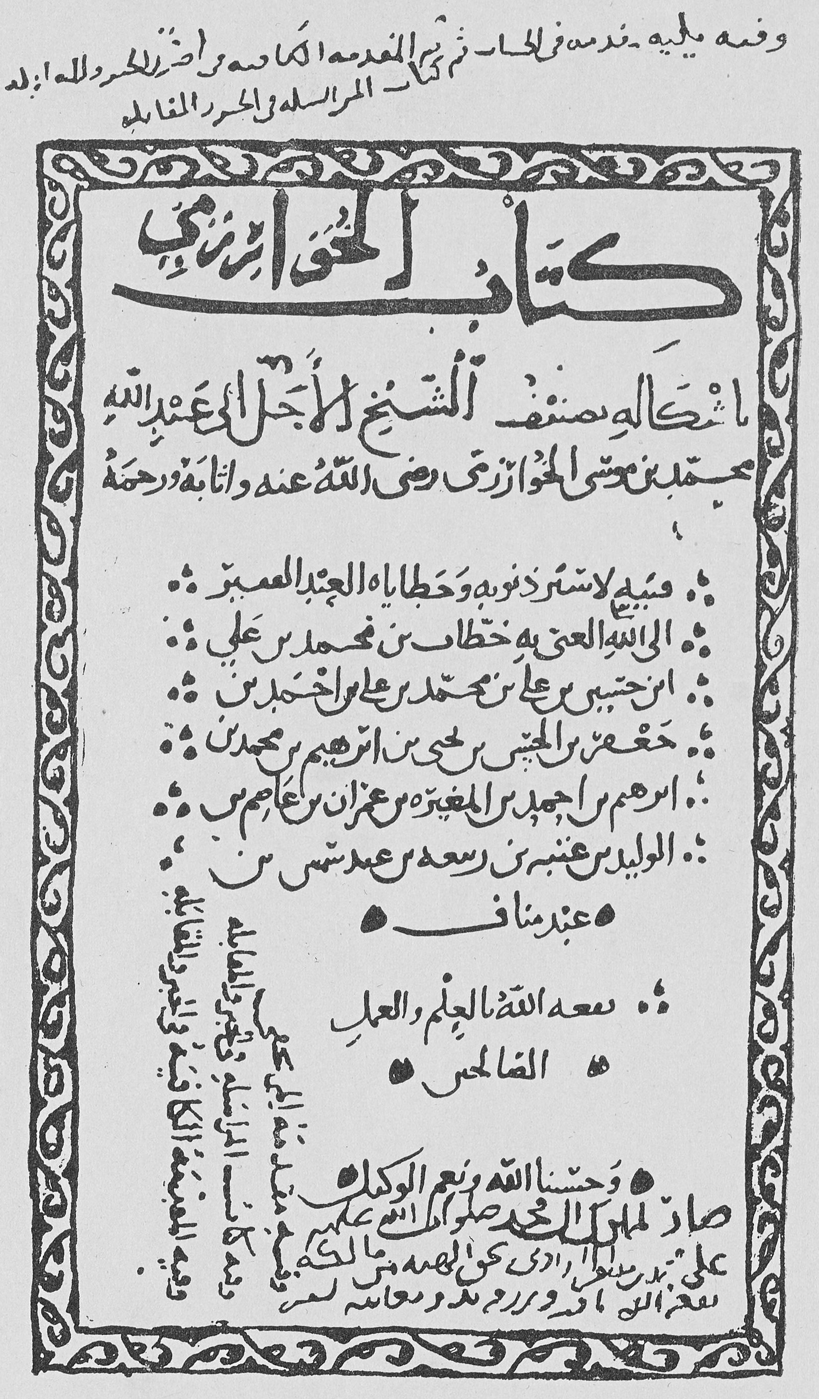
\includegraphics[width=0.8\linewidth,height=0.72\textheight,keepaspectratio]{figures/AK01-F009-FIG1.png}\end{center}\smallskip
\FrameHead{10}{blank}{010}{blank}
\Withheld{blank}
\FrameHead{11}{editors' matter}{011}{editors' matter}
\Withheld{the editors' preface (\RL{\ArBody مقدمة}), first page: a heading and about 20 lines --- not reproduced}
\FrameHead{12}{editors' matter}{012}{editors' matter}
\Withheld{the editors' preface (\RL{\ArBody مقدمة}), second page, with its date and the signatures of the two editors --- not reproduced}
\FrameHead{13}{p. [1]}{013}{p. [\RL{\ArBody ١}]}
\Withheld{the editors' study «\RL{\ArBody الجبر قبل الخوارزمى}» (algebra before al-Khwārizmī): its first page, with the heading --- not reproduced}
\FrameHead{14}{p. 2}{014}{p. \RL{\ArBody ٢}}
\Withheld{the editors' study «\RL{\ArBody الجبر قبل الخوارزمى}» (algebra before al-Khwārizmī), with footnotes --- not reproduced}
\FrameHead{15}{p. 3}{015}{p. \RL{\ArBody ٣}}
\Withheld{the editors' study «\RL{\ArBody الجبر قبل الخوارزمى}» (algebra before al-Khwārizmī), with footnotes --- not reproduced}
\FrameHead{16}{p. 4}{016}{p. \RL{\ArBody ٤}}
\Withheld{the editors' study «\RL{\ArBody الجبر قبل الخوارزمى}» (algebra before al-Khwārizmī), with footnotes --- not reproduced}
\FrameHead{17}{p. 5}{017}{p. \RL{\ArBody ٥}}
\Withheld{the editors' study «\RL{\ArBody الجبر قبل الخوارزمى}» (algebra before al-Khwārizmī), with footnotes --- not reproduced}
\FrameHead{18}{p. 6}{018}{p. \RL{\ArBody ٦}}
\Withheld{the editors' study «\RL{\ArBody الجبر قبل الخوارزمى}» (algebra before al-Khwārizmī), with footnotes --- not reproduced}
\FrameHead{19}{p. 7}{019}{p. \RL{\ArBody ٧}}
\Withheld{the editors' study «\RL{\ArBody الجبر قبل الخوارزمى}» (algebra before al-Khwārizmī), with footnotes --- not reproduced}
\FrameHead{20}{p. 8}{020}{p. \RL{\ArBody ٨}}
\Withheld{the editors' study «\RL{\ArBody الجبر قبل الخوارزمى}» (algebra before al-Khwārizmī), with footnotes --- not reproduced}
\FrameHead{21}{p. 9}{021}{p. \RL{\ArBody ٩}}
\Withheld{the editors' study «\RL{\ArBody الجبر قبل الخوارزمى}» (algebra before al-Khwārizmī), with footnotes --- not reproduced}
\FrameHead{22}{p. [10]}{022}{p. [\RL{\ArBody ١٠}]}
\Withheld{the editors' study, second part, «\RL{\ArBody الخوارزمى}» (al-Khwārizmī: his life and his book): its first page, with the heading, the page number not printed --- not reproduced}
\FrameHead{23}{p. 11}{023}{p. \RL{\ArBody ١١}}
\Withheld{the editors' study, second part (al-Khwārizmī: his life and his book), with footnotes --- not reproduced}
\FrameHead{24}{p. 12}{024}{p. \RL{\ArBody ١٢}}
\Withheld{the editors' study, second part (al-Khwārizmī: his life and his book), with footnotes --- not reproduced}
\FrameHead{25}{p. 13}{025}{p. \RL{\ArBody ١٣}}
\Withheld{the editors' study, second part (al-Khwārizmī: his life and his book), with footnotes --- not reproduced}
\FrameHead{26}{p. 14}{026}{p. \RL{\ArBody ١٤}}
\Withheld{the editors' study, second part (al-Khwārizmī: his life and his book), with footnotes --- not reproduced}
\FrameHead{27}{blank}{027}{blank}
\Withheld{blank}
\FrameHead{28}{plate}{028}{plate}
\par\smallskip\begin{center}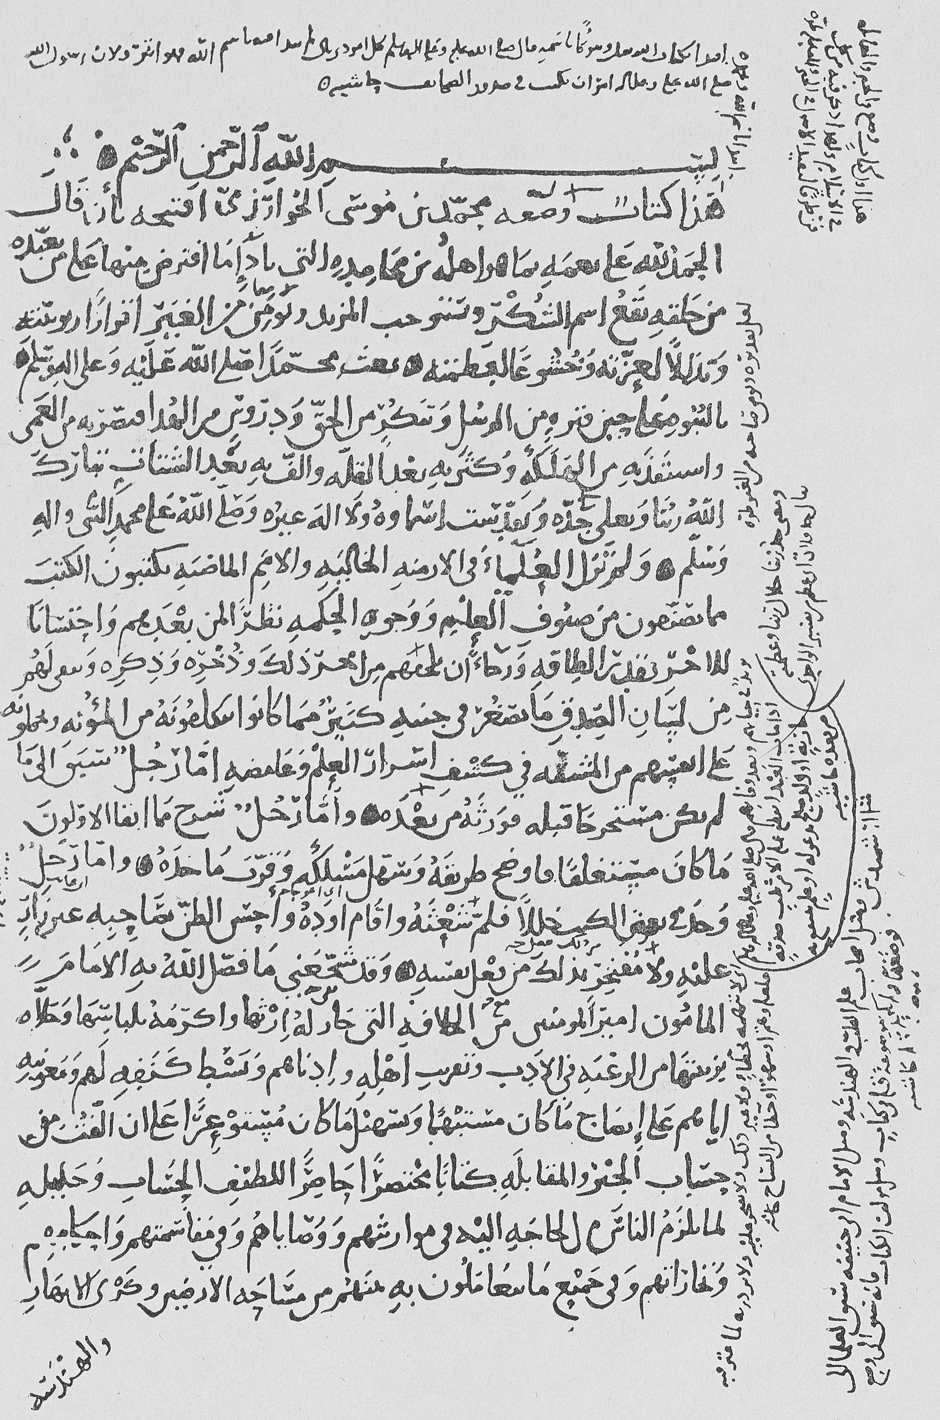
\includegraphics[width=0.8\linewidth,height=0.72\textheight,keepaspectratio]{figures/AK01-F028-FIG1.png}\end{center}\smallskip
\FrameHead{29}{p. [15]}{029}{p. [\RL{\ArBody ١٥}]}
\EdLh{1}{AK01-F029-L01}{بسم الله الرحمن الرحيم}
\EdLp{2}{AK01-F029-L02}{هذا كتاب وضعه محمد بن موسى الخوارزمى افتتحه بأن قال}
\EdLp{3}{AK01-F029-L03}{الحمد لله على نعمه بما هو أهله من محامده التى بأداء ما افترض منها على من}
\EdL{4}{AK01-F029-L04}{يعبده من خلقه يقع اسم الشكر ويستوجب المزيد ونؤمن من الغير اقراراً}
\EdL{5}{AK01-F029-L05}{بربوبيته وتذللا لعزته وخشوعا لعظمته . بعث محمداً صلى الله عليه وعلى آله}
\EdL{6}{AK01-F029-L06}{وسلم بالنبوة على حين فترة من الرسل وتنكر من الحق ودروس من الهدى فبصر}
\EdL{7}{AK01-F029-L07}{به من العمى واستنقذ به من الهلكة وكثر به بعد القلة وألف به بعد الشتات .}
\EdL{8}{AK01-F029-L08}{تبارك الله ربنا وتعالى جده وتقدست أسماؤه ولا إله غيره ، وصلى الله على محمد}
\EdL{9}{AK01-F029-L09}{النبى وآله وسلم . ولم تزل العلماء فى الأزمنة الخالية والأمم الماضية يكتبون}
\EdL{10}{AK01-F029-L10}{الكتب مما يصنفون من صنوف العلم ووجوه الحكمة نظراً لمن بعدهم واحتساباً}
\EdL{11}{AK01-F029-L11}{للأجر بقدر الطاقة ورجاء أن يلحقهم من أجر ذلك وذخره وذكره ويبقى}
\EdL{12}{AK01-F029-L12}{لهم من لسان الصدق ما يصغر فى جنبه كثير مماكانوا يتكلفونه من المؤونة}
\EdL{13}{AK01-F029-L13}{ويحملونه على أنفسهم من المشقة فى كشف أسرار العلم وغامضه . إما رجل}
\EdL{14}{AK01-F029-L14}{سبق إلى مالم يكن مستخرجاً قبله فورثه من بعده . وإما رجل شرح مما أبقى}
\EdL{15}{AK01-F029-L15}{الأولون ما كان مستغلقاً فأوضح طريقه وسهل مسلكه وقرب مأخذه .}
\EdL{16}{AK01-F029-L16}{وإما رجل وجد فى بعض الكتب خللا فلم شعثه وأقام أوده وأحسن الظن}
\EdL{17}{AK01-F029-L17}{بصاحبه غير راد عليه ولا مفتخر بذلك من فعل نفسه . وقد شجعنى ما فضل}
\EdL{18}{AK01-F029-L18}{الله به الامام المأمون أمير المؤمنين مع الخلافة التى حاز له إرثها وأكرمه بلباسها}
\EdL{19}{AK01-F029-L19}{وحلاه بزينتها ، من الرغبة فى الأدب وتقريب أهله وادنائهم وبسط كنفه لهم}
\EdL{20}{AK01-F029-L20}{ومعونته إياهم على إيضاح ماكان مستبهماً وتسهيل ما كان مستوعراً . على أن}
\FrameHead{30}{p. 16}{030}{p. \RL{\ArBody ١٦}}
\EdL{1}{AK01-F030-L01}{ألفت من كتاب الجبر والمقابلة كتاباً مختصراً حاصراً للطيف الحساب وجليله}
\EdL{2}{AK01-F030-L02}{لما يلزم الناس من الحاجة إليه فى مواريثهم ووصاياهم وفى مقاسمتهم وأحكامهم}
\EdL{3}{AK01-F030-L03}{وتجاراتهم ، وفى جميع ما يتعاملون به بينهم من مساحة الأرضين وكرى الأنهار}
\EdL{4}{AK01-F030-L04}{والهندسة وغير ذلك من وجوهه وفنونه ، مقدما لحسن النية فيه وراجيا لأن}
\EdL{5}{AK01-F030-L05}{ينزله أهل الأدب بفضل مااستودعوا من نعم الله تعالى وجليل آلائه وجميل}
\EdL{6}{AK01-F030-L06}{بلائه عندهم منزلته وبالله توفيق فى هذا وفى غيره عليه توكلت وهو رب العرش}
\EdL{7}{AK01-F030-L07}{العظيم . وصلى الله على جميع الانبياء والمرسلين . وإنى لما نظرت فيما يحتاج اليه}
\EdL{8}{AK01-F030-L08}{الناس من الحساب وجدت جميع ذلك عدداً ووجدت جميع الأعداد إنماتركبت}
\EdL{9}{AK01-F030-L09}{من الواحد والواحد داخل فى جميع الأعداد . ووجدت جميع ما يلفظ به من}
\EdL{10}{AK01-F030-L10}{الأعداد ما جاوز الواحد إلى العشرة يخرج مخرج الواحد ثم تثنى العشرةوتثلث}
\EdL{11}{AK01-F030-L11}{كما فعل بالواحد فتكون منها العشرون والثلاثون الى تمام المائة . ثم تثنى المائة}
\EdL{12}{AK01-F030-L12}{وتثلث كما فعل بالواحد وبالعشرة إلى الألف ثم كذلك تردد الألف عند كل}
\EdL{13}{AK01-F030-L13}{عقد إلى غاية المدرك من العدد . ووجدت الأعداد التى يحتاج إليها فى}
\EdL{14}{AK01-F030-L14}{حساب الجبر والمقابلة على ثلاثة ضروب \NoteMark{١} وهى جذور وأموال وعدد مفرد}
\par\smallskip\noindent\rule{30mm}{0.4pt}\Withheld{the editors’ note (\RL{\ArBody ١}), 8 printed lines --- not reproduced}
\FrameHead{31}{p. 17}{031}{p. \RL{\ArBody ١٧}}
\EdL{1}{AK01-F031-L01}{لا ينسب إلى جذر ولا إلى مال . فالجذر منها كل شىء مضروب فى نفسه من}
\EdL{2}{AK01-F031-L02}{الواحد وما فوقه من الأعداد وما دونه من الكسور . والمال كل ما اجتمع}
\EdL{3}{AK01-F031-L03}{من الجذر المضروب فى نفسه . والعدد المفرد كل ملفوظ به من العدد}
\EdL{4}{AK01-F031-L04}{بلا نسبة إلى جذر ولا إلى مال . فمن هذه الضروب الثلاثة ما يعدل بعضها}
\EdL{5}{AK01-F031-L05}{بعضا وهو كقولك أموال تعدل جذوراً . وأموال تعدل عدداً . وجذور}
\EdL{6}{AK01-F031-L06}{تعدل عدداً .}
\EdLp{7}{AK01-F031-L07}{فأما الأموال التى تعدل الجذور فمثل قولك مال يعدل خمسة اجذاره فجذر}
\EdL{8}{AK01-F031-L08}{المال خمسة والمال خمسة وعشرون وهو مثل خمسة أجذاره . وكقولك ثلث مال}
\EdL{9}{AK01-F031-L09}{يعدل أربعة أجذار فالمال كله يعدل اثنى عشر جذراً وهو مائة وأربعة وأربعون}
\EdL{10}{AK01-F031-L10}{وجذره اثنى عشر . ومثل قولك خمسة أموال تعدل عشرة أجذار فالمال الواحد}
\EdL{11}{AK01-F031-L11}{يعدل جذرين وجذر المال اثنان والمال أربعة وكذلك ما كثر من الأموال أو قل}
\EdL{12}{AK01-F031-L12}{يرد إلى مال واحد . وكذلك يفعل بماعادلهامن الأجذار يرد إلى مثل مايرد اليه المال.}
\par\smallskip\noindent\rule{30mm}{0.4pt}\Withheld{the editors’ note (\RL{\ArBody ١}), continued from the page before, 8 printed lines --- not reproduced}
\FrameHead{32}{p. 18}{032}{p. \RL{\ArBody ١٨}}
\EdLp{1}{AK01-F032-L01}{وأما الاموال التى تعدل العدد فمثل قولك مال يعدل تسعة فهو المال وجذره}
\EdL{2}{AK01-F032-L02}{ثلاثةوكقولك خمسةأموال تعدل ثمانين فالمال الواحد خمس الثمانين وهو ستة عشر}
\EdL{3}{AK01-F032-L03}{وكقولك نصف مال يعدل ثمانية عشر فالمال يعدل ستة وثلاثين وجذره ستةوكذلك}
\EdL{4}{AK01-F032-L04}{جميع الأموال زائدها وناقصها ترد إلى مال واحد وإن كانت أقل من مال زيد}
\EdL{5}{AK01-F032-L05}{عليها حتى تكمل مالا تاماً وكذلك يفعل بما عادلها من الأعداد .}
\EdLp{6}{AK01-F032-L06}{وأما الجذور التى تعدل عددا فكقولك جذر يعدل ثلاثة من العدد فالجذر}
\EdL{7}{AK01-F032-L07}{ثلاثة والمال الذى يكون منه تسعة . وكقولك اربعة اجذار تعدل عشرين فالجذر}
\EdL{8}{AK01-F032-L08}{الواحد يعدل خمسة والمال الذى يكون منه خمسة وعشرون وكقولك نصف جذر}
\EdL{9}{AK01-F032-L09}{يعدل عشرة فالجذر يعدل عشرين والمال الذى يكون منه اربعمائة \NoteMark{١}. ووجدت هذه}
\EdL{10}{AK01-F032-L10}{الضروب الثلاثة ، التى هى الجذور والاموال والعدد ، تقترن فيكون منها ثلاثة}
\EdL{11}{AK01-F032-L11}{اجناس مقترنة وهى أموال وجذور تعدل عددا . وأموال وعدد تعدل جذوراً .}
\EdL{12}{AK01-F032-L12}{وجذور وعدد تعدل أموالا . فأما الأموال والجذور التى تعدل العدد فمثل قولك}
\EdL{13}{AK01-F032-L13}{مال وعشرة اجذاره يعدل تسعة وثلاثين درهما ومعناه أى مال اذا زدت عليه مثل}
\EdL{14}{AK01-F032-L14}{عشرةاجذاره بلغ ذلك كله تسعة وثلاثين . فبابه \NoteMark{٢} أن تنصف الأجذار وهى فى}
\par\smallskip\noindent\rule{30mm}{0.4pt}\Withheld{the editors’ notes (\RL{\ArBody ١}) (\RL{\ArBody ٢}), 8 printed lines --- not reproduced}
\FrameHead{33}{p. 19}{033}{p. \RL{\ArBody ١٩}}
\EdL{1}{AK01-F033-L01}{هذه المسئلة خمسة فتضربها فى مثلها فتكون خمسة وعشرين فتزيدها على التسعة}
\EdL{2}{AK01-F033-L02}{والثلاثين فتكون اربعة وستين فتأخذ جذرها وهو ثمانية فتنقص منه نصف}
\EdL{3}{AK01-F033-L03}{الاجذار هو خمسة فيبقى ثلاثة وهوجذر المال الذى تريد والمال تسعة . وكذلك}
\EdL{4}{AK01-F033-L04}{لو ذكر مالين أو ثلاثة أوأقل أو أكثر فاردده إلى مال واحد واردد ما كان معه}
\EdL{5}{AK01-F033-L05}{من الأجذار والعدد إلى مثل ما رددت إليه المال . وهو نحو قولك \NoteMark{١} مالان}
\EdL{6}{AK01-F033-L06}{وعشرة اجذار تعدل ثمانية واربعين درهما ومعناه أى مالين إذا جمعا وزيد عليهما}
\EdL{7}{AK01-F033-L07}{مثل عشرة اجذار احدهما بلغ ذلك ثمانية واربعين درهما فينبغى أن ترد المالين إلى}
\EdL{8}{AK01-F033-L08}{مال واحد وقد علمت أن مالا من مالين نصفهما فاردد كل شىء فى المسئلة إلى نصفه}
\EdL{9}{AK01-F033-L09}{فكأنه قال مال وخمسة اجذار يعدل أربعةوعشرين درهما . ومعناه أى مال إذا}
\EdL{10}{AK01-F033-L10}{زدت عليه خمسة اجذاره بلغ ذلك اربعةوعشرين . فنصف الأجذار فتكون اثنين}
\EdL{11}{AK01-F033-L11}{ونصفا فاضربها فى مثلها فتكون ستة وربعا فزدها على الأربعة والعشرين فتكون}
\EdL{12}{AK01-F033-L12}{ثلاثين درهما وربعا فخذ جذرها وهو خمسة ونصف فانقص منها نصف الأجذار}
\EdL{13}{AK01-F033-L13}{وهو اثنان ونصف يبقى ثلثة وهو جذر المال والمال تسعة . وكذلك \NoteMark{٢} لو قال}
\EdL{14}{AK01-F033-L14}{نصف مال وخمسة أجذاره يعدل ثمانية وعشرين درهما فمعنى ذلك أى مال إذا}
\EdL{15}{AK01-F033-L15}{زدت على نصفه مثل خمسة اجذاره بلغ ذلك ثمانية وعشرين درهما فتريد أن تكمل}
\EdL{16}{AK01-F033-L16}{مالك حتى يبلغ مالا تاماً وهو أن تضعفه فأضعفه وأضعف كلما معك مما يعادله}
\EdL{17}{AK01-F033-L17}{فيكون مالا وعشرة اجذار يعدل ستة وخمسين درهما فنصف الاجذار تكون}
\par\smallskip\noindent\rule{30mm}{0.4pt}\Withheld{the editors’ notes (\RL{\ArBody ١}) (\RL{\ArBody ٢}), 4 printed lines --- not reproduced}
\FrameHead{34}{p. 20}{034}{p. \RL{\ArBody ٢٠}}
\EdL{1}{AK01-F034-L01}{خمسة فاضربها فى مثلها تكون خمسة وعشرين فزدها على الستة والخمسين تكون}
\EdL{2}{AK01-F034-L02}{احدا وثمانين فخذ جذرها وهو تسعة فانقص منها نصف الاجذار وهو \NoteMark{١}خمسة}
\EdL{3}{AK01-F034-L03}{فيبقى أربعة وهو جذر المال الذى أردت والمال ستة عشر ونصفه ثمانية وكذلك}
\EdL{4}{AK01-F034-L04}{فافعل بجميع ما جاءك من الأموال والجذور وما عادلهامن العدد تصب ان شاء الله.}
\EdLp{5}{AK01-F034-L05}{وأما الأموال والعددالتى تعدل الجذور فنحو قولك مال وأحد وعشرون من}
\EdL{6}{AK01-F034-L06}{العدد يعدل عشرة اجذاره ومعناه أى مال إذا زدت عليه واحدا وعشرين درهما}
\EdL{7}{AK01-F034-L07}{كان ما اجتمع مثل عشرة أجذار ذلك المال. فبابه \NoteMark{٢}أن تنصف الاجذار فتكون}
\EdL{8}{AK01-F034-L08}{خمسة فاضربها فى مثلها تكون خمسة وعشرين فأنقص منها الواحد والعشرين التى}
\EdL{9}{AK01-F034-L09}{ذكر انها مع المال فيبقى اربعة فخذ جذرهاوهو اثنان فانقصه من نصف الاجذار}
\EdL{10}{AK01-F034-L10}{وهو خمسة فيبقى ثلاثة وهو جذر المال الذى تريده والمال تسعة . وان شئت}
\EdL{11}{AK01-F034-L11}{فزد الجذر على نصف الاجذار فتكون سبعة وهو جذر المال الذى تريده والمال}
\EdL{12}{AK01-F034-L12}{تسعة واربعون . فاذا وردت عليك مسئلة تخرجك الى هذا الباب فامتحن}
\EdL{13}{AK01-F034-L13}{صوابها بالزيادة فان لم تكن فهى بالنقصان لا محالة وهذا الباب يعمل بالزيادة}
\EdL{14}{AK01-F034-L14}{والنقصان جميعا وليس ذلك فى غيره من الابواب الثلاثة التى يحتاج فيها إلى}
\EdL{15}{AK01-F034-L15}{تنصيف الاجذار . واعلم انك اذا نصفت الاجذار فى هذا الباب وضربتها فى}
\par\smallskip\noindent\rule{30mm}{0.4pt}\Withheld{the editors’ notes (\RL{\ArBody ١}) (\RL{\ArBody ٢}), 6 printed lines --- not reproduced}
\FrameHead{35}{p. 21}{035}{p. \RL{\ArBody ٢١}}
\EdL{1}{AK01-F035-L01}{مثلها فكان مبلغ ذلك أقل من الدراهم التى مع المال فالمسئلة مستحيلة \NoteMark{١}}
\EdL{2}{AK01-F035-L02}{وإن كان مثل الدراهم بعينها \NoteMark{٢} فجذر المال مثل نصف الاجذار سواء}
\EdL{3}{AK01-F035-L03}{لا زيادة ولا نقصان . وكل ما أتاك من مالين أو أكثر أو أقل فاردده الى}
\EdL{4}{AK01-F035-L04}{مال واحد كنحو ما بينت لك فى الباب الاول .}
\EdLp{5}{AK01-F035-L05}{وأما الجذور والعدد التى تعدل الأموال فنحو قولك ثلثة اجذار وأربعةمن}
\EdL{6}{AK01-F035-L06}{العدد تعدل مالا . فبابه أن تنصف الأجذار فتكون واحدا ونصفا فاضربها فى}
\EdL{7}{AK01-F035-L07}{مثلها فتكون اثنين وربعا فزدها على الاربعة فتكون ستةوربعا فخذ جذرهاوهو}
\EdL{8}{AK01-F035-L08}{اثنان ونصف فزده على نصف الأجذار وهو واحد ونصف فتكون اربعة وهوجذر}
\EdL{9}{AK01-F035-L09}{المال ، والمال ستة عشر وكل ماكان اكثر من مال أو أقل فاردده إلى مال واحد}
\EdLp{10}{AK01-F035-L10}{فهذه الستة الضروب التى ذكرتها فى صدر كتابى هذا وقد أتيت على تفسيرها}
\EdL{11}{AK01-F035-L11}{وأخبرت أن منها ثلثة ضروب لا تنصف فيها الأجذار وقد بينت قياسها}
\EdL{12}{AK01-F035-L12}{واضطرارها . فأما ما تحتاج فيه إلى تنصيف الأجذار فى الثلاثة الأبواب الباقية}
\EdL{13}{AK01-F035-L13}{فقد وصفته بأبواب صحيحة وصيرت لكل باب منها صورة يستدل منها على العلة}
\EdL{14}{AK01-F035-L14}{فى التنصيف .}
\EdLp{15}{AK01-F035-L15}{فأما علة مال وعشرة أجذار تعدل تسعة وثلاثين درهما فصورة ذلك سطح}
\par\smallskip\noindent\rule{30mm}{0.4pt}\Withheld{the editors’ notes (\RL{\ArBody ١}) (\RL{\ArBody ٢}), 6 printed lines --- not reproduced}
\FrameHead{36}{p. 22}{036}{p. \RL{\ArBody ٢٢}}
\EdL{1}{AK01-F036-L01}{مربع مجهول الاضلاع وهو المال الذى تريد أن تعرفه وتعرف جذره وهو سطح}
\EdL{2}{AK01-F036-L02}{\Ov{اٮ} وكل ضلع من اضلاعه فهو جذره وكل ضلع من أضلاعه إذا ضربته فى عدد}
\par\smallskip\begin{center}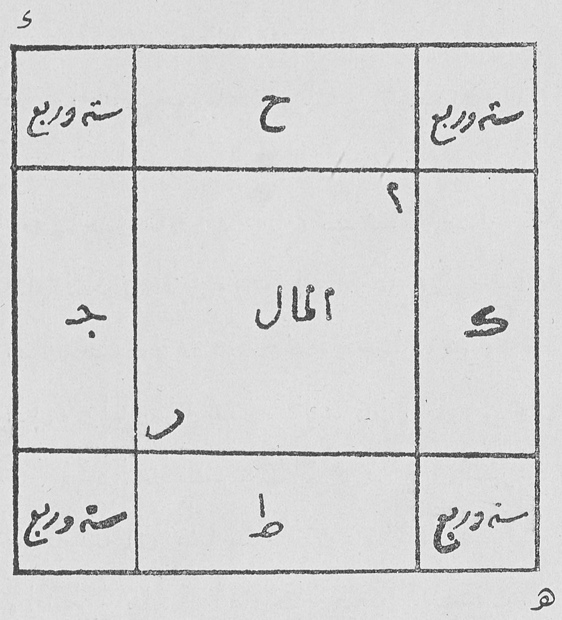
\includegraphics[width=0.6\linewidth,height=0.5\textheight,keepaspectratio]{figures/AK01-F036-FIG1.png}\end{center}\smallskip
\EdL{3}{AK01-F036-L03}{من الأعداد فما بلغت الأعداد}
\EdL{4}{AK01-F036-L04}{فهى اعداد جذور . كل جذر}
\EdL{5}{AK01-F036-L05}{مثل جذر ذلك السطح فلما}
\EdL{6}{AK01-F036-L06}{قيل إن مع المال عشرة اجذاره}
\EdL{7}{AK01-F036-L07}{اخذنا ربع العشرة وهواثنان}
\EdL{8}{AK01-F036-L08}{ونصف وصيرنا كل ربع منها}
\EdL{9}{AK01-F036-L09}{مع ضلع من اضلاع السطح}
\EdL{10}{AK01-F036-L10}{فصار مع السطح الأول الذى}
\EdL{11}{AK01-F036-L11}{هو سطح \Ov{اٮ} اربعة سطوح}
\EdL{12}{AK01-F036-L12}{متساوية طول كل سطح منها}
\EdL{13}{AK01-F036-L13}{مثل جذر سطح \Ov{اٮ} وعرضه اثنان ونصف وهى سطوح ع \Ov{ط} \Ov{ك} ح}
\EdL{14}{AK01-F036-L14}{فحدث سطح متساوى الاضلاع مجهول أيضا ناقص فى زواياه الأربع فى}
\EdL{15}{AK01-F036-L15}{كل زاوية من النقصان اثنان ونصف فى اثنين ونصف فصار الذى يحتاج}
\EdL{16}{AK01-F036-L16}{إليه من الزيادة حتى يتربع السطح اثنان ونصف فى مثله اربع مرات ومبلغ}
\EdL{17}{AK01-F036-L17}{ذلك جميعه خمسة وعشرون . وقد علمنا أن السطح الأول الذى هو سطح المال}
\EdL{18}{AK01-F036-L18}{والأربعة السطوح التى حوله وهى عشرة اجذار هى تسعة وثلاثون من العدد.}
\EdL{19}{AK01-F036-L19}{فاذا زدنا عليها الخمسةوالعشرين التى هى المربعات الاربع التى هى على زواياسطح}
\EdL{20}{AK01-F036-L20}{\Ov{اٮ} تم تربيع السطح الاعظم وهو سطح \Ov{ده} وقد علمنا أن ذلك كله اربعة}
\EdL{21}{AK01-F036-L21}{وستون وأحد أضلاعه جذره وهو ثمانية فاذا نقصنا من الثمانيةمثل ربع العشرة}
\EdL{22}{AK01-F036-L22}{مرتين من طرفى ضلع السطح الأعظم الذى هو سطح \Ov{ده} وهو خمسة بقى من}
\FrameHead{37}{p. 23}{037}{p. \RL{\ArBody ٢٣}}
\EdL{1}{AK01-F037-L01}{ضلعه ثلاثة وهو جذر ذلك المال . وإنما نصفنا العشرة الاجذار وضربناها فى}
\EdL{2}{AK01-F037-L02}{مثلها وزدناها على العدد الذى هو تسعة وثلاثون ليتم لنا بناء السطح الأعظم}
\EdL{3}{AK01-F037-L03}{بما نقص من زواياه الأربع لأن كل عدد يضرب ربعه فى مثله ثم فى أربعة}
\EdL{4}{AK01-F037-L04}{يكون مثل ضرب نصفه فى مثله فاستغنينا بضرب نصف الاجذار فى مثلها عن}
\EdL{5}{AK01-F037-L05}{الربع فى مثله ثم فى أربعة وهذه صورته .}
\EdLp{6}{AK01-F037-L06}{وله أيضا صورة أخرى تؤدى الى هذا وهى سطح \Ov{اٮ} وهو المال فأردنا}
\EdL{7}{AK01-F037-L07}{أن نزيد عليه مثل عشرة أجذاره فنصفنا العشرة فصارت خمسة فصيرناها سطحين}
\EdL{8}{AK01-F037-L08}{على جنبتى سطح \Ov{اٮ} وهما سطحا \Ov{ح} \Inv{ج} فصار طول كل سطح منهما خمسة أذرع}
\EdL{9}{AK01-F037-L09}{وهو نصف العشرة الاجذار وعرضه مثل ضلع سطح \Ov{اٮ} فبقيت لنا مربعة من}
\EdL{10}{AK01-F037-L10}{زوايا سطح \Ov{اٮ} وهى خمسة فى خمسة وهى نصف العشرة الأجذار التى زدناها}
\EdL{11}{AK01-F037-L11}{على جنبتى السطح الأول فعلمنا أن السطح الأول هو المال وأن السطحين اللذين}
\EdL{12}{AK01-F037-L12}{على جنبتيه هما عشرة أجذار فذلك كله تسعة وثلاثون وبقى الى تمام السطح}
\EdL{13}{AK01-F037-L13}{الأعظم مربعة خمسة فى خمسة فذلك خمسة وعشرون فزدناها على تسعة وثلاثين}
\par\smallskip\begin{center}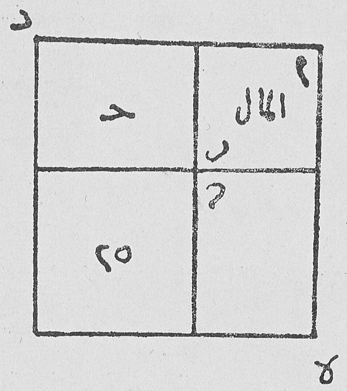
\includegraphics[width=0.6\linewidth,height=0.5\textheight,keepaspectratio]{figures/AK01-F037-FIG1.png}\end{center}\smallskip
\EdL{14}{AK01-F037-L14}{ليتم لنا السطح الأعظم الذى هو سطح \Ov{ده} فبلغ}
\EdL{15}{AK01-F037-L15}{ذلك كله أربعة وستين فأخذنا جذرها وهو}
\EdL{16}{AK01-F037-L16}{ثمانية وهو أحد أضلاع السطح الأعظم فاذا}
\EdL{17}{AK01-F037-L17}{نقصنا منه مثل مازدنا عليه وهو خمسة بقى}
\EdL{18}{AK01-F037-L18}{ثلاثة وهو ضلع سطح \Ov{اٮ} الذى هو المال وهو}
\EdL{19}{AK01-F037-L19}{جذره والمال تسعة وهذه صورته}
\EdLp{20}{AK01-F037-L20}{\Bd{وأما مال وأحد وعشرون درهما تعدل عشرة اجذاره}\NoteMark{١} فا نانجعل المال سطحاً}
\par\smallskip\noindent\rule{30mm}{0.4pt}\Withheld{the editors’ note (\RL{\ArBody ١}), 1 printed line --- not reproduced}
\FrameHead{38}{p. 24}{038}{p. \RL{\ArBody ٢٤}}
\EdL{1}{AK01-F038-L01}{مربعاً مجهول الأضلاع وهو سطح \Ov{اد} ، ثم نضم اليه سطحاً متوازى الأضلاع}
\EdL{2}{AK01-F038-L02}{عرضه مثل أحد أضلاع سطح \Ov{اد} وهو ضلع \Ov{ه\Inv{ن}} والسطح \Ov{هٮ} ، فصار طول}
\EdL{3}{AK01-F038-L03}{السطحين جميعاً ضلع \Ov{حه} ، وقد علمنا أن طوله عشرة من العدد لأن كل سطح}
\EdL{4}{AK01-F038-L04}{مربع متساوى الأضلاع والزوايا فان أحد أضلاعه مضروباً فى واحد جذر ذلك}
\EdL{5}{AK01-F038-L05}{السطح ، وفى اثنين جذراه ، فلما قال مال واحد وعشرون تعدل عشرة أجذاره ،}
\EdL{6}{AK01-F038-L06}{علمنا أن طول ضلع \Ov{هح} عشرة أعداد لأن ضلع \Ov{حد} جذر المال فقسمنا ضلع}
\EdL{7}{AK01-F038-L07}{\Ov{حه} نصفين على نقطة \Ov{ع} فيتبين لنا أن خط \Ov{هع} مثل خط \Ov{عح} وقد تبين}
\EdL{8}{AK01-F038-L08}{لنا أن خط \Ov{عط} مثل خط \Ov{حد} فزدنا على خط \Ov{عط} على استقامته مثل فضل}
\EdL{9}{AK01-F038-L09}{\Ov{حع} على \Ov{عط} ليتربع السطح فصار خط \Ov{طك} مثل خط \Ov{كم} وحدث سطح}
\EdL{10}{AK01-F038-L10}{مربع متساوى الاضلاع والزواياوهو سطح \Ov{مط} وقد كان تبين لنا أن خط \Ov{طك}}
\EdL{11}{AK01-F038-L11}{خمسة وأضلاعه مثله فسطحه إذاً خمسة وعشرون وهو ما اجتمع من ضرب}
\EdL{12}{AK01-F038-L12}{نصف الأجذار فى مثلها وهو خمسة فى خمسة يكون خمسة وعشرين . وقد كان}
\EdL{13}{AK01-F038-L13}{تبين لنا أن سطح \Ov{هٮ} هو الواحد والعشرون التى زيدت على المال فقطعنا من}
\EdL{14}{AK01-F038-L14}{سطح \Ov{هٮ} بخط \Ov{طك} الذى هو أحد أضلاع سطح \Ov{مط} بقى سطح \Ov{طا} وأخذنا}
\EdL{15}{AK01-F038-L15}{من خط \Ov{كم} خط \Ov{كل} وهو مثل خط \Ov{عك} فتبين لنا أن خط \Ov{طع} مثل}
\EdL{16}{AK01-F038-L16}{خط \Ov{مل} وفضل من خط \Ov{مك} خط \Ov{لك} وهو مثل خط \Ov{كع} فصار سطح}
\EdL{17}{AK01-F038-L17}{\Ov{مز} مثل سطح \Ov{طا} فيتبين لنا أن سطح \Ov{هط} مزيدا عليه سطح \Ov{مز}مثل}
\EdL{18}{AK01-F038-L18}{سطح \Ov{هٮ} وهو واحد وعشرون وقد كان سطح \Ov{مط} خمسة وعشرين فلما}
\EdL{19}{AK01-F038-L19}{نقصنا من سطح \Ov{مط} سطح \Ov{هط} وسطح \Ov{مز} اللذين هما واحد وعشرون}
\EdL{20}{AK01-F038-L20}{بقى لنا سطح صغير وهو سطح \Ov{زك} وهو فضل ما بين خمسة وعشرين وواحد}
\EdL{21}{AK01-F038-L21}{وعشرين وهو أربعة وجذرها خط \Ov{زع} وهو مثل خط \Ov{عا} وهو اثنان .}
\EdL{22}{AK01-F038-L22}{فان نقصتهما من خط \Ov{عح} الذى هو نصف الأجذار بقى خط \Ov{اح} وهو}
\FrameHead{39}{plate}{039}{plate}
\par\smallskip\begin{center}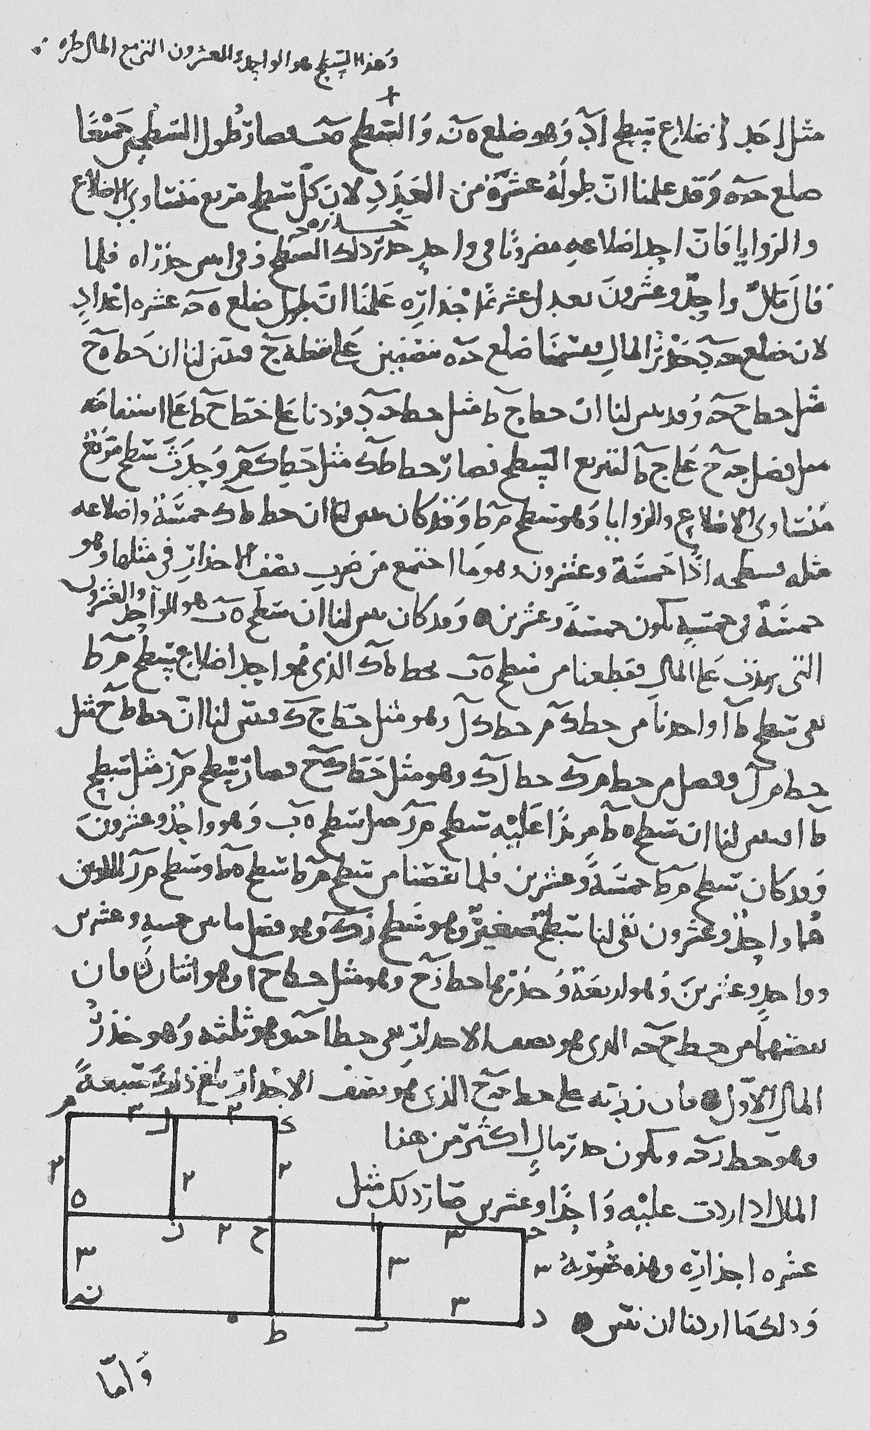
\includegraphics[width=0.8\linewidth,height=0.72\textheight,keepaspectratio]{figures/AK01-F039-FIG1.png}\end{center}\smallskip
\FrameHead{40}{blank}{040}{blank}
\Withheld{blank}
\FrameHead{41}{p. 25}{041}{p. \RL{\ArBody ٢٥}}
\EdL{1}{AK01-F041-L01}{ثلاثة وهو جذر المال الأول . فان زدته على خط \Ov{حع} الذى هو نصف الأجذار}
\EdL{2}{AK01-F041-L02}{بلغ ذلك سبعة وهو خط \Ov{زح} ويكون جذر مال أكثر من هذا المال إذا زدت}
\EdL{3}{AK01-F041-L03}{عليه واحدا وعشرين صار ذلك مثل عشرة أجذاره وهذه صورته \NoteMark{١}}
\EdL{4}{AK01-F041-L04}{وذلك ما أردنا أن نبين}
\par\smallskip\begin{center}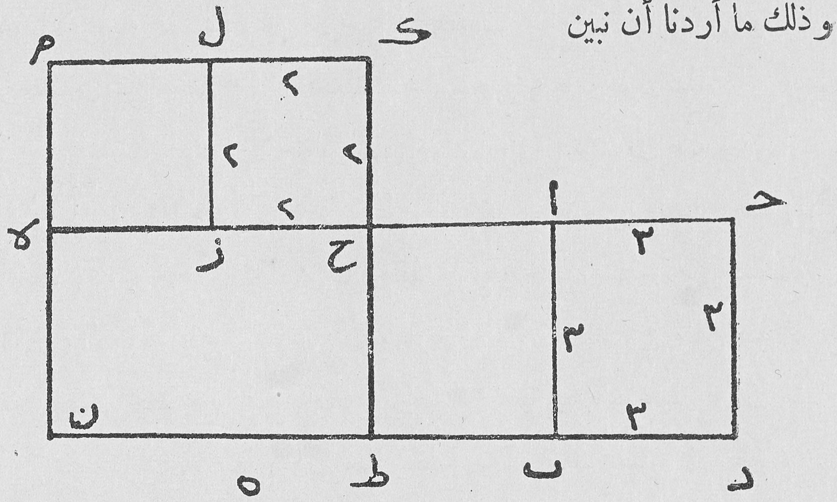
\includegraphics[width=0.6\linewidth,height=0.5\textheight,keepaspectratio]{figures/AK01-F041-FIG1.png}\end{center}\smallskip
\EdLp{5}{AK01-F041-L05}{\Bd{وأما ثلاثة أجذار وأربعة من العدد تعدل مالا} \NoteMark{٢} فانا نجعل المال سطحاً}
\EdL{6}{AK01-F041-L06}{مربعاً مجهول الأضلاع متساوى الأضلاع والزوايا وهوسطح \Ov{اد} فهذا السطح}
\par\smallskip\noindent\rule{30mm}{0.4pt}\Withheld{the editors’ notes (\RL{\ArBody ١}) (\RL{\ArBody ٢}), 9 printed lines --- not reproduced}
\FrameHead{42}{p. 26}{042}{p. \RL{\ArBody ٢٦}}
\EdL{1}{AK01-F042-L01}{كله يجمع الثلاثة الأجذار والأربعة التى ذكرناها وكل سطح مربع فان أحد}
\EdL{2}{AK01-F042-L02}{أضلاعه فى واحد جذره فقطعنا من سطح \Ov{اد} سطح \Ov{هد} فجعلنا أحد أضلاعه}
\EdL{3}{AK01-F042-L03}{الذى هو \Ov{هح} ثلاثة التى هى عدد الأجذار وهى مثل \Ov{زد} فتبين لنا أن سطح}
\EdL{4}{AK01-F042-L04}{\Ov{هٮ} هو الأربعة المزيدة على الأجذار فقطعنا ضلع \Ov{هح} الذى هو ثلاثة}
\EdL{5}{AK01-F042-L05}{أجذار نصفين على نقطة \Ov{ع} ثم جعلنا منه سطحا مربعا وهو سطح \Ov{هط} وهو}
\EdL{6}{AK01-F042-L06}{ما كان من ضرب نصف الأجذار الذى هو واحد ونصف فى مثله وهو اثنان}
\EdL{7}{AK01-F042-L07}{وربع ثم زدنا فى خط \Ov{عط} مثل خط \Ov{اه} وهو خط طل فصار خط \Ov{عل}}
\EdL{8}{AK01-F042-L08}{مثل خط \Ov{اع} وخط \Ov{ك\Inv{ن}} مثل خط \Ov{طل} وحدث سطح مربع متساوى}
\EdL{9}{AK01-F042-L09}{الأضلاع والزوايا وهو سطح \Ov{عم} وقد تبين لنا أن خط \Ov{ع} مثل خط \Ov{مل}}
\EdL{10}{AK01-F042-L10}{وخط \Ov{اع} مثل خط \Ov{عل} فبقى خط \Ov{عح} مثل خط \Ov{\Inv{ن}ز} وخط \Ov{م\Inv{ن}} مثل}
\EdL{11}{AK01-F042-L11}{خط \Ov{طل} فيفضل من سطح \Ov{هٮ} مثل سطح \Ov{كل} وقد علمنا أن سطح \Ov{از}}
\EdL{12}{AK01-F042-L12}{هو الأربعة الزائدة على الثلاثة الاجذار فصار سطح \Ov{ا\Inv{ن}} وسطح \Ov{كل} مثل}
\EdL{13}{AK01-F042-L13}{سطح \Ov{از} الذى هو الاربعة العدد فتبين لنا أن سطح \Ov{عم} هو نصف الاجذار}
\par\smallskip\begin{center}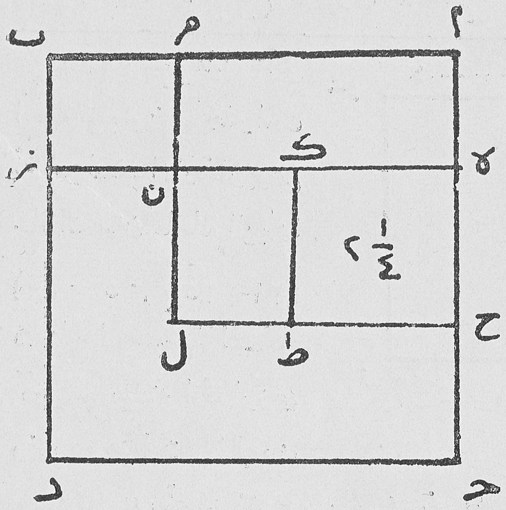
\includegraphics[width=0.6\linewidth,height=0.5\textheight,keepaspectratio]{figures/AK01-F042-FIG1.png}\end{center}\smallskip
\EdL{14}{AK01-F042-L14}{الذى هو واحد ونصف فى مثله}
\EdL{15}{AK01-F042-L15}{وهو اثنان وربع وزيادة الأربعة}
\EdL{16}{AK01-F042-L16}{التى هى سطح \Ov{ا\Inv{ن}} وسطح \Ov{كل} وقد}
\EdL{17}{AK01-F042-L17}{بقى لنا من ضلع المربعة الأوله التى}
\EdL{18}{AK01-F042-L18}{هى سطح \Ov{اد} وهو المال كله نصف}
\EdL{19}{AK01-F042-L19}{الاجذار وهو واحد ونصف وهو}
\EdL{20}{AK01-F042-L20}{خط \Ov{عح} فاذا زدناه على خط \Ov{اع}}
\EdL{21}{AK01-F042-L21}{الذى هو جذر سطح \Ov{عم} اثنان}
\FrameHead{43}{p. 27}{043}{p. \RL{\ArBody ٢٧}}
\EdL{1}{AK01-F043-L01}{ونصف وزدنا عليه خط \Ov{عح} الذى هو نصف الثلاثة الاجذار وهو واحد}
\EdL{2}{AK01-F043-L02}{ونصف فبلغ ذلك كله أربعة وهو خط \Ov{اح} وهو جذر المال الذى هو سطح \Ov{اد}}
\EdL{3}{AK01-F043-L03}{وهذه صورته وذلك ما أردنا أن نبين .}
\EdLp{4}{AK01-F043-L04}{ووجدنا كل ما يعمل به من حساب الجبر والمقابلة لا بد أن يخرجك الى أحد}
\EdL{5}{AK01-F043-L05}{الأبواب الستة التى وصفت فى كتابى هذا وقد أتيت على تفسيرها فاعرف ذلك .}
\EdL{6}{AK01-F043-L06}{\Bd{باب الضرب} وأنا مخبرك كيف تضرب الأشياء وهى الجذور بعضها فى بعض}
\EdL{7}{AK01-F043-L07}{اذا كانت منفردة ، أو كان معها عدد ، أو كان مستثنى منها عدد ، أو كانت مستثناة}
\EdL{8}{AK01-F043-L08}{من عدد ، وكيف تجمع بعضها الى بعض ، وكيف تنقص بعضها من بعض . أعلم}
\EdL{9}{AK01-F043-L09}{انه لا بد لكل عدد يضرب فى عدد من أن يضاعف أحد العددين بقدر ما فى}
\EdL{10}{AK01-F043-L10}{الآخر من الآحاد . فاذا كانت عقود ومعها آحاد أو مستثنى منها آحاد فلا بد من}
\EdL{11}{AK01-F043-L11}{ضربها أربع مرات . العقود فى العقود ، والعقود فى الآحاد ، والآحاد فى العقود ،}
\EdL{12}{AK01-F043-L12}{والآحاد فى الآحاد . فاذا كانت الآحاد التى مع العقود زائدة جميعاً فالضرب الرابع}
\EdL{13}{AK01-F043-L13}{زائد،واذا كانت ناقصة جميعا فالضرب الرابع زائد أيضاً، واذاكان أحدهما زائدا}
\EdL{14}{AK01-F043-L14}{والآخر ناقصاً فالضرب الرابع ناقص \NoteMark{١} وهو مثل عشرةوواحد فى عشرة واثنين \NoteMark{٢}}
\EdL{15}{AK01-F043-L15}{فالعشرة فى العشرة مائة والواحد فى العشرة عشرة زائدة والاثنان فى العشرة}
\EdL{16}{AK01-F043-L16}{عشرون زائدةوالواحد فى الاثنين اثنان زائدان فذلك كله مائة واثنان وثلاثون واذا}
\EdL{17}{AK01-F043-L17}{كانت عشرة الا واحداً فى عشرة الا واحداً \NoteMark{٣} فالعشرة فى العشرة مائة والواحد}
\par\smallskip\noindent\rule{30mm}{0.4pt}\Withheld{the editors’ notes (\RL{\ArBody ١}) (\RL{\ArBody ٢}) (\RL{\ArBody ٣}), 4 printed lines --- not reproduced}
\FrameHead{44}{p. 28}{044}{p. \RL{\ArBody ٢٨}}
\EdL{1}{AK01-F044-L01}{الناقص فى العشرة عشرة ناقصة والواحد الناقص أيضا فى العشرة عشرة ناقصة}
\EdL{2}{AK01-F044-L02}{فذلك ثمانون والواحد الناقص فى الواحد الناقص واحد زائد فذلك أحد وثمانون.}
\EdL{3}{AK01-F044-L03}{واذا كانت عشرة واثنان فى عشرة الا واحداً \NoteMark{١} فالعشرة فى العشرة مائة}
\EdL{4}{AK01-F044-L04}{والواحد الناقص فى العشرةعشرةناقصةوالاثنان الزائدان فى العشرةعشرون زائدة}
\EdL{5}{AK01-F044-L05}{فذلك مائة وعشرة والاثنان الزائدان فى الواحد المنقوص اثنان ناقصان فذلك}
\EdL{6}{AK01-F044-L06}{كله مائة وثمانية . وإنما بينت ذلك لتستدل به على ضرب الأشياء بعضها فى بعض}
\EdL{7}{AK01-F044-L07}{اذا كان معها عدد أو استثنيت من عدد أو استثنى منها عدد . فاذا قيل لك عشرة}
\EdL{8}{AK01-F044-L08}{الا شيئا ومعنى الشىء الجذر فى عشرة \NoteMark{٢} فاضرب عشرة فى عشرة يكون مائة}
\EdL{9}{AK01-F044-L09}{والا شيئا فى عشرة يكون عشرة أجذار ناقصة فيعدل مائة الا عشرة أشياء . فان}
\EdL{10}{AK01-F044-L10}{قال عشرة وشىء فى عشرة فاضرب عشرة فى عشرة يكون مائة وشيئا فى عشرة}
\EdL{11}{AK01-F044-L11}{بعشرة أشياء زائدة يكون مائة وعشرة أشياء . وان قال عشرة وشىء فى مثلها \NoteMark{٣}}
\EdL{12}{AK01-F044-L12}{قلت عشرة فى عشرة مائة وعشرةفى شىء بعشرةأشياء وعشرةفى شىء بعشرة أشياء}
\EdL{13}{AK01-F044-L13}{أيضا وشىء فى شىء مال زائد فيكون ذلك مائة درهم وعشرين شيئا ومالا زائداً .}
\EdL{14}{AK01-F044-L14}{وإن قال عشرة الا شيئاً فى عشرة الا شيئاً \NoteMark{٤} قلت عشرة فى عشرة بمائة والا}
\EdL{15}{AK01-F044-L15}{شيئاً فى عشرة عشرة أشياء ناقصة والا شيئا فى عشرة عشرة أشياء ناقصة والا}
\EdL{16}{AK01-F044-L16}{شيئاً فى الا شيئاً مال زائد فيكون ذلك مائة ومالا الا عشرين شيئاً \NoteMark{٥} وكذلك}
\par\smallskip\noindent\rule{30mm}{0.4pt}\Withheld{the editors’ notes (\RL{\ArBody ١}) (\RL{\ArBody ٢}) (\RL{\ArBody ٣}) (\RL{\ArBody ٤}) (\RL{\ArBody ٥}), 5 printed lines --- not reproduced}
\FrameHead{45}{p. 29}{045}{p. \RL{\ArBody ٢٩}}
\EdL{1}{AK01-F045-L01}{لو أنه قال لك درهم إلا سدساً فى درهم الا سدساً يكون خمسة أسداس فى مثلها}
\EdL{2}{AK01-F045-L02}{وهى خمسة وعشرين جزءاً من ستة وثلاثين من أجزاء الدرهم وهو ثلثان وسدس}
\EdL{3}{AK01-F045-L03}{السدس وقياسه أن تضرب درهما فى درهم فيكون درهما ( والا سدساً فى درهم}
\EdL{4}{AK01-F045-L04}{بسدس ناقص والا سدساً فى درهم بسدس ناقص فيبقى ثلثان والا سدساً فى}
\EdL{5}{AK01-F045-L05}{سدس \NoteMark{١} بسدس السدس زائداً وذلك ثلثان وسدس السدس ) ثم درهم فى الا}
\EdL{6}{AK01-F045-L06}{سدساً بسدس ناقص ثم درهم فى الا سدسا بسدس ناقص فيكون ثلثى درهم والا}
\EdL{7}{AK01-F045-L07}{سدسا فى الا سدس بسدس السدس زائد فذلك ثلثان وسدس السدس وان قال}
\EdL{8}{AK01-F045-L08}{عشرة الا شيئا فى عشرة وشىء \NoteMark{٢} قلت عشرة فى عشرة مائةوالا شيئاً فى عشرة}
\EdL{9}{AK01-F045-L09}{عشرةأشياءناقصةوشىءفى عشرةعشرةأشياءزائدةوالا شيئاًفى شىءمال ناقص فيكون}
\EdL{10}{AK01-F045-L10}{لك مائة درهم الا مالا . وإن قال عشرةالا شيئاً فى شىء قلت عشرةفى شىء عشرة}
\EdL{11}{AK01-F045-L11}{أشياء والا شيئاً فى شىء مال ناقص فيكون عشرة أشياء الا مالا وان قال عشرة}
\EdL{12}{AK01-F045-L12}{وشىء فى شىء الا عشرة قلت شىء فى عشرة عشرةأشياء زائدة وشىء فى شىء مال}
\EdL{13}{AK01-F045-L13}{زائد والا عشرة فى عشرة مائة درهم ناقصةوالا عشرةفى شىء بعشرةأشياءناقصة}
\EdL{14}{AK01-F045-L14}{فتقول مال الا مائة درهم بعد ما قابلت به وذلك أن تطرح عشرة أشياء زائدة}
\EdL{15}{AK01-F045-L15}{بعشرة أشياء ناقصة فيبقى مال الا مائة درهم . وان قال عشرةدراهم ونصف شىء}
\EdL{16}{AK01-F045-L16}{فى نصف درهم الا خمسة أشياء \NoteMark{٣} قلت نصف درهم فى عشرةبخمسةدراهم زائدة}
\EdL{17}{AK01-F045-L17}{ونصف درهم فى نصف شىء بربع شىء زائد والا خمسة أشياء فى عشرة دراهم}
\EdL{18}{AK01-F045-L18}{خمسون جذراً ناقصة فيكون جميع ذلك خمسة دراهم الا تسعة وأربعين جذراً}
\par\smallskip\noindent\rule{30mm}{0.4pt}\Withheld{the editors’ notes (\RL{\ArBody ١}) (\RL{\ArBody ٢}) (\RL{\ArBody ٣}), 4 printed lines --- not reproduced}
\FrameHead{46}{p. 30}{046}{p. \RL{\ArBody ٣٠}}
\EdL{1}{AK01-F046-L01}{( شيئاً ) وثلاثة أرباع جذر ثم تضرب خمسة أجذار ناقصة فى نصف جذر زائد}
\EdL{2}{AK01-F046-L02}{فيكون مالين ونصفا ناقصاً فذلك خمسة دراهم الا مالين ونصفا والا تسعة}
\EdL{3}{AK01-F046-L03}{وأربعين جذراً وثلاثة أرباع جذر . فان قال عشرة وشىء فى شىء الا عشرة فكانه}
\EdL{4}{AK01-F046-L04}{قال شىء وعشرة فى شىء الا عشرة فتقول شىء فى شىء مال زائد وعشرة فى شىء}
\EdL{5}{AK01-F046-L05}{عشرة أشياء زائدة والا عشرة فى شىءعشرةأشياء ناقصةفذهبت الزيادة بالنقصان}
\EdL{6}{AK01-F046-L06}{وبقى المال والا عشرة فى عشرة مائة منقوصة من المال فجميع ذلك مال الا مائة}
\EdL{7}{AK01-F046-L07}{درهم . وكل ما كان من الضرب زائداً وناقصاً مثل الأشياءفى زيادةشىءفالضرب}
\EdL{8}{AK01-F046-L08}{الأخير ناقص أبداً فاعلم ذلك وبالله التوفيق . \Bd{باب الجمع والنقصان} اعلم أن جذر}
\EdL{9}{AK01-F046-L09}{مائتين الا عشرة مجموع الى عشرين الا جذر مائتين فانه عشرة سوياً \NoteMark{١} .}
\EdL{10}{AK01-F046-L10}{وجذر مائتين الا عشرة منقوص من عشرين الا جذر مائتين فهو ثلاثون الا}
\EdL{11}{AK01-F046-L11}{جذرى مائتين . وجذرا مائتين هوجذر ثمانى مائة . ومائة ومال الا عشرين جذراً}
\EdL{12}{AK01-F046-L12}{مجموع اليه خمسون وعشرة أجذارالا مالين \NoteMark{٢} فهو مائة ( ومال ) وخمسون الا مالا}
\EdL{13}{AK01-F046-L13}{والا عشرةأجذار \NoteMark{٣} . ومائةومال الى عشرين جذراً منقوص منه خمسون وعشرة}
\EdL{14}{AK01-F046-L14}{أجذار الا مالين فهو خمسون درهما وثلاثة أموال الا ثلاثين جذراً . وأنامبين لك}
\EdL{15}{AK01-F046-L15}{علة ذلك فى صورة تؤدى الى الطلب ان شاء الله تعالى . واعلم أن كل جذر مال}
\EdL{16}{AK01-F046-L16}{معلوم أو أصم تريد أن تضعفه ومعنى اضعافك إياه أن تضربه فى اثنين فينبغى}
\par\smallskip\noindent\rule{30mm}{0.4pt}\Withheld{the editors’ notes (\RL{\ArBody ١}) (\RL{\ArBody ٢}) (\RL{\ArBody ٣}), 6 printed lines --- not reproduced}
\FrameHead{47}{p. 31}{047}{p. \RL{\ArBody ٣١}}
\EdL{1}{AK01-F047-L01}{أن تضرب اثنين فى اثنين ثم فى المال فيصير جذر ما اجتمع مثلى جذر ذلك المال}
\EdL{2}{AK01-F047-L02}{وان أردت ثلاثة أمثاله فاضرب ثلاثة فى ثلاثة ثم فى المال فيكون جذر ما اجتمع}
\EdL{3}{AK01-F047-L03}{ثلاثة أمثال جذر ذلك المال الأول وكذلك مازاد من الأضعاف أو نقص فعلى}
\EdL{4}{AK01-F047-L04}{هذا المثال نفسه \NoteMark{١} . وان أردت أن تأخذ نصف جذر مال فينبغى أن تضرب}
\EdL{5}{AK01-F047-L05}{نصفاً فى نصف فيكون ربعاً ثم فى المال فيكون جذر ما اجتمع مثل نصف جذر}
\EdL{6}{AK01-F047-L06}{ذلك المال . وكذلك ثلثه أو ربعه أو أقل من ذلك أو أكثر بالغاً مابلغ فى النقصان}
\EdL{7}{AK01-F047-L07}{والاضعاف : \Bd{ومثال ذلك} اذا أردت أن تضعف جذر تسعةضربت اثنين فى اثنين}
\EdL{8}{AK01-F047-L08}{ثم فى تسعة فيكون ذلك ستة وثلاثين فخذ جذرها يكون ستة وهو كجذر تسعة \NoteMark{٢}}
\EdL{9}{AK01-F047-L09}{وكذلك لوأردت أن تضعف جذر تسعة ثلاث مرات ضربت ثلاثة فى ثلاثة ثم}
\EdL{10}{AK01-F047-L10}{فى تسعة فيكون أحد وثمانين فخذ جذرها تسعة وذلك جذر تسعة مضاعفاً ثلاث}
\EdL{11}{AK01-F047-L11}{مرات . فان أردت أن تأخذ نصف جذر تسعة فانك تضرب نصفاً فى}
\EdL{12}{AK01-F047-L12}{نصف فيكون ربعا ثم تضرب ربعاً فى تسعة فيكون اثنين وربعاً فتأخذ جذرها}
\EdL{13}{AK01-F047-L13}{وهو واحد ونصف وهو نصف جذر تسعة وكذلك ما زاد أو نقص من}
\EdL{14}{AK01-F047-L14}{المعلوم والاصم . فهذا طريقه . \Bd{القسم} \NoteMark{٣} وان أردت أن تقسم جذر تسعةعلى جذر}
\EdL{15}{AK01-F047-L15}{أربعة \NoteMark{٤} فانك تقسم تسعة على اربعة فيكون اثنين وربعا فجذرها هو ما يصيب}
\par\smallskip\noindent\rule{30mm}{0.4pt}\Withheld{the editors’ notes (\RL{\ArBody ١}) (\RL{\ArBody ٢}) (\RL{\ArBody ٣}) (\RL{\ArBody ٤}), 5 printed lines --- not reproduced}
\FrameHead{48}{p. 32}{048}{p. \RL{\ArBody ٣٢}}
\EdL{1}{AK01-F048-L01}{الواحد وهو واحد ونصف . وان أردت أن تقسم جذر أربعة على جذر تسعة}
\EdL{2}{AK01-F048-L02}{فانك تقسم أربعة على تسعة فيكون اربعة اتساع واحد فجذرها ما يصيب الواحد}
\EdL{3}{AK01-F048-L03}{وهو ثلثا واحد . فان اردت أن تقسم جذرى تسعة على جذر اربعة أو غيرها}
\EdL{4}{AK01-F048-L04}{من الاموال فاضعف جذر التسعة على ما أريتك فى عمل الاضعاف فما بلغ}
\EdL{5}{AK01-F048-L05}{فاقسمه على أربعة أو على ما اردت أن تقسم عليه واعمل به كما عملت . وكذلك}
\EdL{6}{AK01-F048-L06}{ان أردت ثلاثة أجذار تسعة أو اكثر أو نصف جذر تسعة أوأقل أو ما كان}
\EdL{7}{AK01-F048-L07}{فعلى هذا المنوال فاعمله تصب ان شاء الله تعالى . وان اردت أن تضرب جذر}
\EdL{8}{AK01-F048-L08}{تسعة فى جذر اربعة\NoteMark{١} فاضرب تسعة فى أربعة فيكون ستة وثلاثين فخذ جذرها}
\EdL{9}{AK01-F048-L09}{وهو ستةفهو جذر تسعة مضروب فى جذر أربعة . وكذلك لوأردت أن تضرب}
\EdL{10}{AK01-F048-L10}{جذر خمسة فى جذر عشرة فاضرب خمسة فى عشرة فجذر ما بلغ هو الشىء الذى}
\EdL{11}{AK01-F048-L11}{تريده . وان اردت ان تضرب جذر ثلث فى جذر نصف فاضرب ثلثا فى نصف}
\EdL{12}{AK01-F048-L12}{فيكون سدسا فجذر السدس هو جذر الثلث مضروب فى جذر النصف .}
\EdL{13}{AK01-F048-L13}{وان اردت أن تضرب جذرى تسعة فى ثلاثة أجذار اربعة فاستخرج جذرى}
\EdL{14}{AK01-F048-L14}{تسعة كما وصفت لك حتى تعلم جذر أى مال هو وكذلك فافعل بثلاثة اجذار}
\EdL{15}{AK01-F048-L15}{الاربعة حتى تعلم جذر أى مال هو ثم اضرب المالين أحدهما فى الآخر فجذر}
\EdL{16}{AK01-F048-L16}{ما اجتمع لك هو جذر \NoteMark{٢} تسعة فى ثلاثة أجذار اربعة وكذلك كلما زاد من}
\EdL{17}{AK01-F048-L17}{الأجذار أونقص فعلى هذا المثال فاعمل به \Bd{فأما عز} جذر مائتين الا عشرة}
\EdL{18}{AK01-F048-L18}{مجموعا الى عشرين الا جذر مائتين فان صورة ذلك خط \Ov{اٮ} وهو جذر مائتين}
\EdL{19}{AK01-F048-L19}{فمن ا الى نقطة ح هو العشرة والباقى جذر مائتين هو الباقى من خط \Ov{اٮ}}
\EdL{20}{AK01-F048-L20}{وهو خط \Ov{حٮ} ثم تخرج من نقطة \Ov{ٮ} خطا الى نقطة \Ov{ه} وهو خط العشرين وهو}
\par\smallskip\noindent\rule{30mm}{0.4pt}\Withheld{the editors’ notes (\RL{\ArBody ١}) (\RL{\ArBody ٢}), 2 printed lines --- not reproduced}
\FrameHead{49}{p. 33}{049}{p. \RL{\ArBody ٣٣}}
\EdL{1}{AK01-F049-L01}{مثلا خط \Ov{اح} الذى هو عشرة فمن نقطة \Ov{ٮ} الى نقطة \Ov{ه} مثل خط \Ov{اٮ} فهو جذر}
\EdL{2}{AK01-F049-L02}{مائتين أيضا والباقى من العشرين هو من نقطة \Ov{ه} الى نقطة \Ov{د} فلما أردنا أن نجمع}
\EdL{3}{AK01-F049-L03}{مابقى من جذر المائتين بعد طرح العشرة وهو خط \Ov{حٮ} الى خط \Ov{هد} الذى هو}
\EdL{4}{AK01-F049-L04}{عشرون الا جذر مائتين فقطعنا من خط \Ov{ٮه} مثل خط \Ov{حٮ} وهو خط \Ov{زه} وقد}
\EdL{5}{AK01-F049-L05}{كان تبين لنا أن خط \Ov{اٮ} الذى هو جذرمائتين مثل خط \Ov{ٮه} وأن خط \Ov{اح} الذى}
\EdL{6}{AK01-F049-L06}{هو العشرة مثل خط \Ov{ٮز} والباقى من خط \Ov{اٮ} الذى هو \Ov{حٮ} مثل الباقى من خط}
\EdL{7}{AK01-F049-L07}{\Ov{ٮه} الذى هو \Ov{زه} زدنا على خط \Ov{هد} خط \Ov{زه} فتبين لنا أنه قد نقص من خط \Ov{ٮد}}
\EdL{8}{AK01-F049-L08}{الذى هو عشرون مثل خط \Ov{اح} الذى هوعشرة وهو خط \Ov{ٮز} وبقى لناخط \Ov{زد}}
\par\smallskip\begin{center}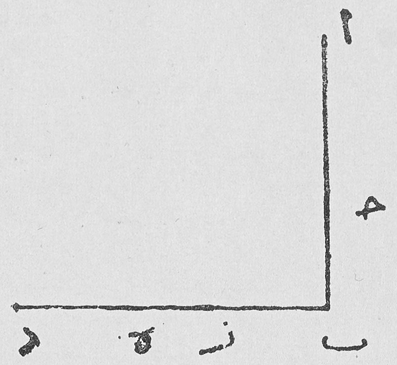
\includegraphics[width=0.6\linewidth,height=0.5\textheight,keepaspectratio]{figures/AK01-F049-FIG1.png}\end{center}\smallskip
\EdL{9}{AK01-F049-L09}{وهوعشرة وذلك ما أردنا أن نبين وهذه}
\EdL{10}{AK01-F049-L10}{صورته . وأما علة جذر مائتين الا عشرة}
\EdL{11}{AK01-F049-L11}{منقوصاً من عشرين الا جذر مائتين فان}
\EdL{12}{AK01-F049-L12}{صورة ذلك خط \Ov{اٮ} وهو جذر مائتين}
\EdL{13}{AK01-F049-L13}{ومن \Ov{ا} الى نقطة \Ov{ح} هى العشرة المعلومة}
\EdL{14}{AK01-F049-L14}{ونخرج من نقطة \Ov{ٮ} خطا الى نقطة \Ov{د}}
\EdL{15}{AK01-F049-L15}{ونجعله العشرين ونجعل من \Ov{ٮ} الى نقطة \Ov{ه}}
\EdL{16}{AK01-F049-L16}{مثل خط جذر مائتين وهو مثل خط \Ov{اٮ} وقد تبين لنا أن خط \Ov{حٮ} هو مابقى}
\EdL{17}{AK01-F049-L17}{من جذر مائتين بعد القاء العشرة وخط \Ov{ده} هو مابقى من العشرين بعد القاء}
\EdL{18}{AK01-F049-L18}{جذر المائتين فأردنا أن ننقص خط \Ov{حٮ} من خط \Ov{هد} فأخرجنا من نقطة \Ov{ٮ}}
\EdL{19}{AK01-F049-L19}{خطا الى نقطة \Ov{ر} وهو مثل خط \Ov{اح} الذى هو العشرة فصار جميع خط \Ov{رد} مثل}
\EdL{20}{AK01-F049-L20}{خط \Ov{رٮ} وخط \Ov{ٮد} وقد تبين لنا أن ذلك كله ثلاثون وقطعنا من خط \Ov{هد} مثل}
\EdL{21}{AK01-F049-L21}{خط \Ov{حٮ} وهو خط \Ov{هح} فتبين لنا أن خط \Ov{حد} هو مابقى من خط \Ov{رد} الذى}
\FrameHead{50}{p. 34}{050}{p. \RL{\ArBody ٣٤}}
\EdL{1}{AK01-F050-L01}{هو ثلاثون وتبين لنا أن خط \Ov{ٮه} جذر مائتين وخط \Ov{رٮ} و\Ov{ٮح} جذر المائتين}
\EdL{2}{AK01-F050-L02}{أيضاً فلما صار خط \Ov{هع} مثل خط \Ov{حٮ} تبين لنا أن الذى نقص من خط \Ov{رد}}
\EdL{3}{AK01-F050-L03}{— الذى هو ثلاثون — جذرا مائتين وجذرا مائتين هو جذر ثمانى مائة وذلك}
\par\smallskip\begin{center}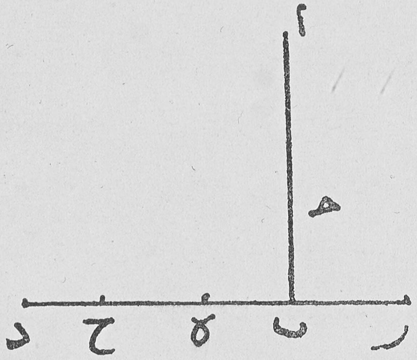
\includegraphics[width=0.6\linewidth,height=0.5\textheight,keepaspectratio]{figures/AK01-F050-FIG1.png}\end{center}\smallskip
\EdL{4}{AK01-F050-L04}{ما أردنا أن نبين وهذه صورته . وأما}
\EdL{5}{AK01-F050-L05}{مائةومال الاعشرين جذراًمجموع اليه خمسون}
\EdL{6}{AK01-F050-L06}{وعشرة أجذار الا مالين فلم تستقم له}
\EdL{7}{AK01-F050-L07}{صورة لأنه من ثلاثة أجناس مختلفة . أموال}
\EdL{8}{AK01-F050-L08}{وجذوروعدد وليس معها مايعادلها فتصور}
\EdL{9}{AK01-F050-L09}{وقد تمكننالهاصورة لاتحسن فامااضطرارها}
\EdL{10}{AK01-F050-L10}{باللفظ فبين وذلك أنك قد علمت أن معك مائةومالاالا عشرين جذرافلمازدت عليها}
\EdL{11}{AK01-F050-L11}{خمسين وعشرةأجذار صارت مائةوخمسين ومالا الا عشرة أجذار لأن هذه العشرة}
\EdL{12}{AK01-F050-L12}{الاجذارالمزيدةجبرت من العشرين الجذر الناقصةعشرةأجذارفبقيت مائةوخمسون}
\EdL{13}{AK01-F050-L13}{ومال الا عشرة أجذار وقد كان مع المائة مال فلما نقصت من المائة والمال المالين}
\EdL{14}{AK01-F050-L14}{المستثنين من الخمسين ذهب مال بمال وبقى عليك مال فصارت مائةوخمسين الا مالا}
\EdL{15}{AK01-F050-L15}{والا عشرة أجذار وذلك ما أردنا أن نبين . \Bd{باب المسائل الست} وقد قدمنا قبل}
\EdL{16}{AK01-F050-L16}{أبواب الحساب ووجوهها ست مسائل جعلتها أمثلة للستة الأبواب المتقدمة فى}
\EdL{17}{AK01-F050-L17}{صدر كتابى هذا لابد ان منها ثلاثة لاتنصف فيها الأجذار وذكرت أن حساب}
\EdL{18}{AK01-F050-L18}{الجبر والمقابلة لابد أن يخرجك الى باب منها ثم اتبعت ذلك من المسائل بما يقرب}
\EdL{19}{AK01-F050-L19}{من الفهم وتخف فيه المؤنةوتسهل فيه الدلالةان شاء الله تعالى . \Bd{فالاولى من الست}}
\EdL{20}{AK01-F050-L20}{نحو قولك عشرة قسمتها قسمين فضربت أحد القسمين فى الآخر ثم ضربت}
\EdL{21}{AK01-F050-L21}{أحدهما فى نفسه فصار المضروب فى نفسه مثل أحد القسمين فى الآخر اربع}
\FrameHead{51}{p. 35}{051}{p. \RL{\ArBody ٣٥}}
\EdL{1}{AK01-F051-L01}{مرات \NoteMark{١} فقياسه أن تجعل أحد القسمين شيئا والآخر عشرة الا شيئا فتضرب}
\EdL{2}{AK01-F051-L02}{شيئا فى عشرة الا شيئا فتكون عشرة أشياء الا مالا ثم تضربه فى أربعة لقولك}
\EdL{3}{AK01-F051-L03}{أربع مرات فيكون أربعة أمثال المضروب من أحد القسمين والآخر فيكون}
\EdL{4}{AK01-F051-L04}{ذلك أربعين شيئا الا اربعة أموال ثم تضرب شيئا فى شىء وهو أحدالقسمين فى}
\EdL{5}{AK01-F051-L05}{نفسه فيكون مالا يعدل أربعين شيئا الا أربعة أموال فاجبرها بالأربعةالأموال}
\EdL{6}{AK01-F051-L06}{وزدها على المال فيكون أربعين شيئا تعدل خمسة أموال فالمال الواحديعدل ثمانية}
\EdL{7}{AK01-F051-L07}{أجذار وهو أربعة وستون جذرها ثمانية وهو أحد القسمين المضروب فى نفسه}
\EdL{8}{AK01-F051-L08}{والباقى من العشرة اثنان وهو القسم الآخر فقد أخرجتك هذه المسألة الى أحد}
\EdL{9}{AK01-F051-L09}{الأبواب الستة وهى أموال تعدل جذوراً فاعلم ذلك \NoteMark{٢} . \Bd{والمسألة الثانية} عشرة}
\EdL{10}{AK01-F051-L10}{قسمتها قسمين فضربت كل قسم فى نفسه ثم ضربت العشرة فى نفسها فكان مااجتمع}
\EdL{11}{AK01-F051-L11}{من ضرب العشرة فى نفسها مثل أحد القسمين مضروبا فى نفسه مرتين وسبعة}
\EdL{12}{AK01-F051-L12}{اتساع مرة أو مثل الآخر مضروباً فى نفسه ست مرات وربع مرة\NoteMark{٣}. فقياس ذلك}
\EdL{13}{AK01-F051-L13}{ان تجعل أحد القسمين شيئاً والآخر عشرة الا شيئا فتضرب الشىء فى نفسه}
\EdL{14}{AK01-F051-L14}{فيكون مالا ثم فى اثنين وسبعة اتساع فيكون مالين وسبعة اتساع مال ثم تضرب}
\EdL{15}{AK01-F051-L15}{العشرة فى مثلها فتكون مائة تعدل مالين وسبعة اتساع مال فاردده الى مال واحد}
\par\smallskip\noindent\rule{30mm}{0.4pt}\Withheld{the editors’ notes (\RL{\ArBody ١}) (\RL{\ArBody ٢}) (\RL{\ArBody ٣}), 7 printed lines --- not reproduced}
\FrameHead{52}{p. 36}{052}{p. \RL{\ArBody ٣٦}}
\EdL{1}{AK01-F052-L01}{وهو تسعة أجزاء من خمسة وعشرين جزءا وهو خمس وأربعة أخماس الخمس فخذ}
\EdL{2}{AK01-F052-L02}{خمس المائة وأربعة أخماس خمسها وهو ستة وثلاثون تعدل مالا فخذ جذرهاستة}
\EdL{3}{AK01-F052-L03}{وهو أحد القسمين والآخر أربعة لامحالة فقد أخرجتك هذه المسألة الى أحد}
\EdL{4}{AK01-F052-L04}{الأبواب الستة وهى أموال تعدل عددا . \Bd{والمسألة الثالثة} عشرة قسمتها قسمين}
\EdL{5}{AK01-F052-L05}{ثم قسمت أحدهما على الآخر فخرج القسم أربعة \NoteMark{١} . فقياس ذلك أن تجعل أحد}
\EdL{6}{AK01-F052-L06}{القسمين شيئا والآخر عشرة الا شيئا ثم تقسم عشرة الا شيئاً على شىء ليكون}
\EdL{7}{AK01-F052-L07}{أربعة وقد علمت انك متى ماضربت ما خرج لك من القسم فى المقسوم عليه عاد}
\EdL{8}{AK01-F052-L08}{المال الذى قسمته والقسم فى هذه المسألة أربعة والمقسوم عليه شىء فاضرب}
\EdL{9}{AK01-F052-L09}{أربعة فى شىء فيكون أربعة أشياء تعدل المال الذى قسمته وهو عشرة الا شيئا}
\EdL{10}{AK01-F052-L10}{فاجبر العشرة بالشىء وزده على الأربعة الاشياء فيكون خمسة أشياء تعدل}
\EdL{11}{AK01-F052-L11}{عشرة فالشىء الواحد اثنان وهو أحد القسمين فقد أخرجتك هذه المسألةالى}
\EdL{12}{AK01-F052-L12}{أحد الأبواب الستة وهى جذور تعدل عدداً . \Bd{والمسألة الرابعة} مال ضربت ثلثه}
\EdL{13}{AK01-F052-L13}{ودرهما فى ربعه ودرهم فكان عشرين \NoteMark{٢} . قياسه أن تضرب ثلث شىءفى ربع شىء}
\EdL{14}{AK01-F052-L14}{فيكون نصف سدس مال وتضرب درهمافى ثلث شىءفيكون ثلث شىءودرهمافى}
\EdL{15}{AK01-F052-L15}{ربع شىء بربع شىء ودرهما فى درهم بدرهم فذلك كله نصف سدس مال وثلث شىء}
\par\smallskip\noindent\rule{30mm}{0.4pt}\Withheld{the editors’ notes (\RL{\ArBody ١}) (\RL{\ArBody ٢}), 6 printed lines --- not reproduced}
\FrameHead{53}{p. 37}{053}{p. \RL{\ArBody ٣٧}}
\EdL{1}{AK01-F053-L01}{وربع شىء ودرهم تعدل عشرين درهما فالق من العشرين درهما بدرهم فتبقى تسعة}
\EdL{2}{AK01-F053-L02}{عشر درهما تعدل نصف سدس مال وثلث شىء وربع شىء فكمل مالك واكماله}
\EdL{3}{AK01-F053-L03}{أن تضرب كل ما معك فى اثنى عشر فيصير معك مال وسبعة أجذار}
\EdL{4}{AK01-F053-L04}{تعدل مائتين وثمانية وعشرين درهما فنصف الاجذار واضربها فى مثلها}
\EdL{5}{AK01-F053-L05}{تكن اثنى عشر وربعاً فزدها على الاعداد وهى مائتان وثمانية وعشرين فيكون}
\EdL{6}{AK01-F053-L06}{مائتين واربعين وربعا فخذ جذرها خمسة عشر ونصفاً فانقص منه نصف الأجذار}
\EdL{7}{AK01-F053-L07}{وهو ثلاثة ونصف يبقى اثنى عشر وهو المال فقد أخرجتك هذه المسئلة الى أحد}
\EdL{8}{AK01-F053-L08}{الأبواب الستةوهى أموال وجذور تعدل عدداً. \Bd{والمسألة الخامسة} عشرة قسمتها}
\EdL{9}{AK01-F053-L09}{قسمين ثم ضربت كل قسم فى نفسه وجمعتهما فكانا ثمانيةوخمسين درهما \NoteMark{١} . قياسه}
\EdL{10}{AK01-F053-L10}{أن تجعل أحد القسمين شيئا والآخر عشرة الا شيئا فاضرب عشرة الا شيئا فى}
\EdL{11}{AK01-F053-L11}{مثلها فيكون مائة ومالا الا عشرين شيئاً ثم تضرب شيئا فى شىء فيكون مالا ثم}
\EdL{12}{AK01-F053-L12}{تجمعهما فيكون ذلك مائةومالين الاعشرين شيئا تعدل ثمانية وخمسين درهما فاجبر}
\EdL{13}{AK01-F053-L13}{المائة والمالين بالعشرين الشىء الناقصة وزدها على الثمانية والخمسين فيكون مائة}
\EdL{14}{AK01-F053-L14}{ومالين تعدل ثمانية وخمسين درهما وعشرين شيئاً فاردد ذلك الى مال واحد وهو}
\EdL{15}{AK01-F053-L15}{أن تأخذ نصف مامعك فيكون خمسين درهماً ومالا تعدل تسعةوعشرين درهماً}
\EdL{16}{AK01-F053-L16}{وعشرة أشياء فقابل به وذلك أنك تلقى من الخمسين تسعة وعشرين فيبقى أحد}
\EdL{17}{AK01-F053-L17}{وعشرون ومال تعدل عشرة أشياء فنصف الاجذار يكون خمسة واضربها فى مثلها}
\par\smallskip\noindent\rule{30mm}{0.4pt}\Withheld{the editors’ note (\RL{\ArBody ١}), 3 printed lines --- not reproduced}
\FrameHead{54}{p. 38}{054}{p. \RL{\ArBody ٣٨}}
\EdL{1}{AK01-F054-L01}{فتكون خمسة وعشرين فالق منها الواحد والعشرين التى مع المال فيبقى أربعة فخذ}
\EdL{2}{AK01-F054-L02}{جذرها وهو اثنان فانقصه من نصف الاجذار التى هى خمسة \NoteMark{١} يبقى ثلاثة وهى}
\EdL{3}{AK01-F054-L03}{أحد القسمين والآخر سبعة فقد أخرجتك هذه المسألة الى أحد الأبواب الستة}
\EdL{4}{AK01-F054-L04}{وهى أموال وعدد تعدل جذوراً . \Bd{والمسألة السادسة} (مال)ضربت ثلثه فى ربعه}
\EdL{5}{AK01-F054-L05}{فعاد (المال) وزيادة اربعة وعشرين درهما \NoteMark{٢} . فقياسه أن تجعل مالك شيئا ثم}
\EdL{6}{AK01-F054-L06}{تضرب ثلث شىء فى ربع شىء فيكون نصف سدس مال تعدل شيئا وأربعة}
\EdL{7}{AK01-F054-L07}{وعشرين درهما ثم تضرب نصف سدس المال فى اثنى عشر حتى تكمل مالك}
\EdL{8}{AK01-F054-L08}{واضرب الشىء فى اثنى عشر يكن اثنى عشر شيئا واضرب الاربعة والعشرين فى}
\EdL{9}{AK01-F054-L09}{اثنى عشر فيصير معك مائتان وثمانية وثمانون درهما واثنى عشر جذرا تعدل مالا}
\EdL{10}{AK01-F054-L10}{فنصف الاجذار تكون ستة واضربها فى مثلها وزدها على مائتين وثمانية وثمانين}
\EdL{11}{AK01-F054-L11}{فيكون ثلثمائة واربعة وعشرين فخذ جذرها وهو ثمانية عشر فزده على نصف}
\EdL{12}{AK01-F054-L12}{الاجذار وهى ستة فيكون ذلك أربعة وعشرين وهو (المال) فقد أخرجتك هذه}
\EdL{13}{AK01-F054-L13}{المسئلة الى أحد الأبواب الستة وهى جذور وعدد تعدل أموالا .}
\EdL{14}{AK01-F054-L14}{\Bd{باب المسائل المختلفة} . فان سأل سائل فقال عشرة قسمتها قسمين ثم ضربت}
\EdL{15}{AK01-F054-L15}{أحدهما فى الآخر فكان واحداً وعشرين درهما\NoteMark{٣}. فقد علمت أن أحد القسمين}
\par\smallskip\noindent\rule{30mm}{0.4pt}\Withheld{the editors’ notes (\RL{\ArBody ١}) (\RL{\ArBody ٢}) (\RL{\ArBody ٣}), 6 printed lines --- not reproduced}
\FrameHead{55}{p. 39}{055}{p. \RL{\ArBody ٣٩}}
\EdL{1}{AK01-F055-L01}{من العشرة شىء والآخر عشرة الا شيئا فاضرب شيئا فى عشرة الا شيئا فيكون}
\EdL{2}{AK01-F055-L02}{عشرةأشياءالامالا تعدل أحداًوعشرين فاجبرالعشرةالأشياءبالمال وزده على الواحد}
\EdL{3}{AK01-F055-L03}{والعشرين فيكون عشرة أشياء تعدل أحداً وعشرين درهما ومالا فالق نصف}
\EdL{4}{AK01-F055-L04}{الأجذار فيبقى خمسة فاضربها فى مثلها تكن خمسة وعشرين فالق منها الواحد}
\EdL{5}{AK01-F055-L05}{والعشرين التى مع المال فيبقى أربعة فخذ جذرها وهو اثنان فانقصه من نصف}
\EdL{6}{AK01-F055-L06}{الأجذار وهى خمسة يبقى ثلاثة وذلك أحد القسمين . وان شئت زدت جذر}
\EdL{7}{AK01-F055-L07}{الأربعة على نصف الأجذار فتكون سبعة وهو أحد القسمين وهذه المسألة التى}
\EdL{8}{AK01-F055-L08}{تعمل بالزيادة والنقصان . \Bd{وان قال} عشرة قسمتها قسمين فضربت كل قسم فى}
\EdL{9}{AK01-F055-L09}{نفسه ثم القيت الأقل من الاكثر فبقى أربعون \NoteMark{١} قياسه أن تضرب عشرة}
\EdL{10}{AK01-F055-L10}{الا شيئا فى مثلها فتكون مائةومالا الا عشرين شيئا وتضرب شيئا فى شىء فيكون}
\EdL{11}{AK01-F055-L11}{مالا فانقصه من المائة والمال الا عشرين شيئا تبقى مائة الا عشرين شيئا تعدل}
\EdL{12}{AK01-F055-L12}{أربعين درهما فاجبر المائة بالعشرين الشىء وزدها على الأربعين فيكون مائة تعدل}
\EdL{13}{AK01-F055-L13}{عشرين شيئا وأربعين درهما فالق الأربعين من المائة يبقى ستون درهما تعدل عشرين}
\EdL{14}{AK01-F055-L14}{شيئا فالشىءالواحد يعدل ثلاثة وهوأحد القسمين .\Bd{وان قال} عشرة قسمتها قسمين}
\EdL{15}{AK01-F055-L15}{فضربت كل قسم فى نفسه وجمعتهما وزدت عليهما فضل مابين القسمين من قبل أن}
\EdL{16}{AK01-F055-L16}{تضربهما فبلغ ذلك أربعة وخمسين درهما \NoteMark{٢} .فان قياسه أن تضرب عشرة الا شيئا}
\EdL{17}{AK01-F055-L17}{فى متلها فتكون مائة ومالا الاعشرين شيئا وتضرب الشىء الباقى من العشرة فى مثله}
\par\smallskip\noindent\rule{30mm}{0.4pt}\Withheld{the editors’ notes (\RL{\ArBody ١}) (\RL{\ArBody ٢}), 4 printed lines --- not reproduced}
\FrameHead{56}{p. 40}{056}{p. \RL{\ArBody ٤٠}}
\EdL{1}{AK01-F056-L01}{فيكون مالا ثم تجمع ذلك فيكون مائة ومالين الا عشرين شيئا وقال زدت عليهما}
\EdL{2}{AK01-F056-L02}{فضل مابينهما قبل أن تضربهما فقلت فضل مابينهما عشرة الا شيئين فجميع ذلك}
\EdL{3}{AK01-F056-L03}{مائةوعشرةومالان الااثنتين وعشرين شيئا يعدل أربعةوخمسين درهمافاذا جبرت}
\EdL{4}{AK01-F056-L04}{وقابلت قلت مائةوعشرةدراهم ومالان تعدل أربعةوخمسين درهماواثنين وعشرين}
\EdL{5}{AK01-F056-L05}{شيئا فاردد المالين الى مال واحد وهو أن تأخذ نصف ما معك فيكون خمسة}
\EdL{6}{AK01-F056-L06}{وخمسين درهما ومالا تعدل سبعة وعشرين درهما وأحد عشر شيئا فالق سبعة}
\EdL{7}{AK01-F056-L07}{وعشرين من خمسةوخمسين يبقى ثمانيةوعشرون درهما ومالا تعدل أحدعشرشيئا}
\EdL{8}{AK01-F056-L08}{فنصف الأشياء فيكون خمسةونصف فاضربهافى مثلها فيكون ثلاثين وربعا فانقص}
\EdL{9}{AK01-F056-L09}{منها الثمانيةوالعشرين التى مع المال فبقى اثنان وربع فخذ جذرها وهو واحد ونصف}
\EdL{10}{AK01-F056-L10}{فانقصه من نصف الأجذار يبقى اربعة وهوأحد القسمين.\Bd{فان قال} عشرة قسمتها}
\EdL{11}{AK01-F056-L11}{قسمين فقسمت هذا على هذا وهذا على هذا فبلغ \NoteMark{١} ذلك درهمين وسدساً .}
\EdL{12}{AK01-F056-L12}{فقياس ذلك \NoteMark{٢} أنك اذا ضربت كل قسم فى نفسه ثم جمعتهما كان مثل أحد}
\EdL{13}{AK01-F056-L13}{القسمين اذا ضربت احداهما فى الآخر ثم ضربت الذى اجتمع معك من الضرب}
\EdL{14}{AK01-F056-L14}{فى الذى بلغ القسم وهو اثنان وسدس فاضرب عشرة الا شيئا فى مثلها يكن مائة}
\EdL{15}{AK01-F056-L15}{ومالا الا عشرين شيئا واضرب شيئا فى شىء فيكون مالا فاجمع ذلك فيصير مائة}
\par\smallskip\noindent\rule{30mm}{0.4pt}\Withheld{the editors’ notes (\RL{\ArBody ١}) (\RL{\ArBody ٢}), 7 printed lines --- not reproduced}
\FrameHead{57}{p. 41}{057}{p. \RL{\ArBody ٤١}}
\EdL{1}{AK01-F057-L01}{ومالين الا عشرين شيئا يعدل شيئا مضروبا فى عشرة الا شيئاوذلك عشرة أشياء}
\EdL{2}{AK01-F057-L02}{الا مالا مضروبا فى ماخرج من القسمين وهو اثنان وسدس فيكون ذلك أحداً}
\EdL{3}{AK01-F057-L03}{وعشرين شيئا وثلثى شىء الا مالين وسدسا تعدل مائة ومالين الا عشرين شيئا}
\EdL{4}{AK01-F057-L04}{فاجبر ذلك وزد مالين وسدساً على مائة ومالين الاعشرين شيئاوزدالعشرين الشىء}
\EdL{5}{AK01-F057-L05}{الناقصة من المائة والمالين على الواحد والعشرين الشىء وثلثى الشىء فيكون معك}
\EdL{6}{AK01-F057-L06}{مائة وأربعة أموال وسدس مال تعدل أحدا وأربعين شيئا وثلثى شىء فاردد ذلك}
\EdL{7}{AK01-F057-L07}{الى مال وقد علمت أن المال الواحد من أربعة أموال وسدس هو خمسها وخمس}
\EdL{8}{AK01-F057-L08}{خمسها فخذ من جميع مامعك الخمس وخمس الخمس فيكون معك أربعة وعشرون}
\EdL{9}{AK01-F057-L09}{ومال تعدل عشرة أجذار لأن العشرة من أحد وأربعين شيئا وثلثى شىء خمسها}
\EdL{10}{AK01-F057-L10}{وخمس خمسها فنصف الأجذار وهو خمسة واضربها فى مثلها فيكون خمسة}
\EdL{11}{AK01-F057-L11}{وعشرين فانقص منها الأربعة والعشرين التى مع المال يبقى واحد فخذ جذره وهو}
\EdL{12}{AK01-F057-L12}{واحد فانقصه من نصف الأجذار وهى خمسة يبقى أربعة وهو أحد}
\EdL{13}{AK01-F057-L13}{القسمين . واعلم بأن كل شيئين تقسم هذا على هذا وهذا على هذا فانك}
\EdL{14}{AK01-F057-L14}{اذا ضربت الذى يخرج من هذا فى الذى، يخرج من هذا كان واحدا}
\EdL{15}{AK01-F057-L15}{أبدا \NoteMark{١} \Bd{فان قال} عشرة قسمتها قسمين وضربت أحد القسمين فى خمسة وقسمته}
\EdL{16}{AK01-F057-L16}{على الآخر ثم القيت نصف ما اجتمع معك وزدته على المضروب فى خمسة فكان}
\EdL{17}{AK01-F057-L17}{خمسين درهما \NoteMark{٢} فان قياس ذلك أن تأخذ شيئا من العشرة فتضربه فى خمسة}
\par\smallskip\noindent\rule{30mm}{0.4pt}\Withheld{the editors’ notes (\RL{\ArBody ١}) (\RL{\ArBody ٢}), 5 printed lines --- not reproduced}
\FrameHead{58}{p. 42}{058}{p. \RL{\ArBody ٤٢}}
\EdL{1}{AK01-F058-L01}{فيكون خمسة أشياء مقسومة على الباقى من العشرة وهو عشرة الا شيئا مأخوذ}
\EdL{2}{AK01-F058-L02}{نصفها ومعلوم أنك اذا قسمت الخمسة الأشياء على عشرةالاشيئا وأخذت نصف}
\EdL{3}{AK01-F058-L03}{ماخرج كان ذلك كقسمك نصف الخمسة الأشياء على العشرةإلاشيئا فاذا أخذت}
\EdL{4}{AK01-F058-L04}{نصف الخمسة الأشياء صار شيئين ونصفا وهو الذى تريد أن تقسمه على عشرة}
\EdL{5}{AK01-F058-L05}{الا شيئا يخرج يعدل خمسين الا خمسة أشياء لأنه قال تضم اليه أحد القسمين}
\EdL{6}{AK01-F058-L06}{مضروبا فى خمسة فيكون ذلك كله خمسين وقد علمت انك متى ضربت ما خرج}
\EdL{7}{AK01-F058-L07}{لك من القسم فى المقسوم عليه عاد المال ومالك شيئان ونصف فاضرب عشرة}
\EdL{8}{AK01-F058-L08}{الا شيئا فى خمسين الا خمسة أشياء فيكون ذلك خمسمائة درهم وخمسة أموال}
\EdL{9}{AK01-F058-L09}{الا مائة شىء تعدل شيئين ونصفا فاردد ذلك الى مال واحد فيكون ذلك مائة}
\EdL{10}{AK01-F058-L10}{درهم ومالاالا عشرين شيئا تعدل نصف شىء فاجبرذلك المائةوزدالعشرين الشىء}
\EdL{11}{AK01-F058-L11}{على نصف الشىء فيصير معك مائة درهم ومال تعدل عشرين شيئا ونصف شىء}
\EdL{12}{AK01-F058-L12}{فنصف الأشياء واضربها فى مثلها وانقص منها المائة وخذ جذرمابقى وانقصه من}
\EdL{13}{AK01-F058-L13}{نصف الأجذار وهو عشرة وربع فيبقى ثمانية وهو أحد القسمين . \Bd{فان قال}}
\EdL{14}{AK01-F058-L14}{عشرة قسمتها قسمين فضربت أحد القسمين فى نفسه فكان مثل الآخر}
\EdL{15}{AK01-F058-L15}{احدى وثمانين مرة \NoteMark{١} . فقياس ذلك أن تقول عشرة الا شيئافى مثلهابمائة ومال}
\EdL{16}{AK01-F058-L16}{الا عشرين شيئا تعدل احدا وثمانين شيئا فاجبر المائة والمال بالعشرين الشىء وزدها}
\EdL{17}{AK01-F058-L17}{على الواحد والثمانين ( الشىء ) فيكون مائة ومالا تعدل مائة جذرا وجذرا}
\EdL{18}{AK01-F058-L18}{فنصف الأجذار فتكون خمسين ونصفا واضربها فى مثلها فيكون الفين وخمسمائة}
\par\smallskip\noindent\rule{30mm}{0.4pt}\Withheld{the editors’ note (\RL{\ArBody ١}), 3 printed lines --- not reproduced}
\FrameHead{59}{p. 43}{059}{p. \RL{\ArBody ٤٣}}
\EdL{1}{AK01-F059-L01}{وخمسين وربعا فانقص منها المائة فيبقى الفان واربعمائة وخمسون وربع}
\EdL{2}{AK01-F059-L02}{فخذ جذرها وهو تسعة وأربعون ونصف فانقصها من نصف الأجذار وهو}
\EdL{3}{AK01-F059-L03}{خمسون ونصف فيبقى واحد وهو أحد القسمين . \Bd{فان قال} عشرةأقفزة حنطة}
\EdL{4}{AK01-F059-L04}{أو شعيرا بعت كل واحد منهما بسعر \NoteMark{١} ثم جمعت ثمنهما فكان ما اجتمع مثل}
\EdL{5}{AK01-F059-L05}{فضل مابين السعرين ومثل مابين الكيلين فخذ ماشئت فانه يجوز \NoteMark{٢} فكأنك}
\EdL{6}{AK01-F059-L06}{أخذت أربعة وستة فقلت بعت كل واحد من الأربعة بشىء فضربت أربعة}
\EdL{7}{AK01-F059-L07}{فى شىء فصار أربعة أشياء وبعت الستة كل واحد بمثل نصف الشىء الذى بعت}
\EdL{8}{AK01-F059-L08}{به الأربعة وان شئت بثلثه وان شئت بربعه أو ما شئت فانه يجوز . فاذا كان}
\EdL{9}{AK01-F059-L09}{بيعك الآخر بنصف شىء فاضرب نصف شىء فى ستة فيكون ثلاثة أشياء}
\EdL{10}{AK01-F059-L10}{فاجمعها مع الاربعة الاشياء فتكون سبعة أشياء تعدل مابين الكيلين وهو}
\EdL{11}{AK01-F059-L11}{قفيزان وفضل مابين السعرين وهو نصف شىء فيكون سبعة أشياء تعدل اثنين}
\EdL{12}{AK01-F059-L12}{ونصف شىء فالق نصف شىء من سبعة أشياء فتبقى ستة أشياء ونصف ( شىء )}
\EdL{13}{AK01-F059-L13}{تعدل درهمين فالشىء الواحد أربعة أجزاء من ثلاثة عشر فتقول باع الاربعة}
\par\smallskip\noindent\rule{30mm}{0.4pt}\Withheld{the editors’ notes (\RL{\ArBody ١}) (\RL{\ArBody ٢}), 8 printed lines --- not reproduced}
\FrameHead{60}{p. 44}{060}{p. \RL{\ArBody ٤٤}}
\EdL{1}{AK01-F060-L01}{كل واحد بأربعة أجزاء من ثلاثة عشر من درهم وباع الستة كل واحد بجزأين}
\EdL{2}{AK01-F060-L02}{من ثلاثة عشر من درهم فبلغ ذلك ثمانية وعشرين جزءا من ثلاثة عشر من درهم}
\EdL{3}{AK01-F060-L03}{وذلك مثل فضل ما بين الكيلين وهو قفيزان فصرفهما ستة وعشرون جزءا}
\EdL{4}{AK01-F060-L04}{وفضل ما بين السعرين وهو جزءان فذلك ثمانية وعشرون جزءا . \Bd{فان قال}}
\EdL{5}{AK01-F060-L05}{مالان بينهما درهمان قسمت القليل على الكثير فأصاب القسم نصف درهم \NoteMark{١}}
\EdL{6}{AK01-F060-L06}{فاجعل أحد المالين شيئا والآخر شيئا ودرهمين فلما قسمت شيئا على شىء}
\EdL{7}{AK01-F060-L07}{ودرهمين خرج القسم نصف درهم وقد علمت أنك متى ضربت ما خرج لك}
\EdL{8}{AK01-F060-L08}{من القسم فى المقسوم عليه عاد مالك الذى قسمته وهو شىء فقل شىء ودرهمان}
\EdL{9}{AK01-F060-L09}{فى النصف الذى هو القسم فيكون نصف شىء ودرهما تعدل شيئا فألقيت}
\EdL{10}{AK01-F060-L10}{نصف شىء بنصف شىء وبقى درهم يعدل نصف شىء فاضعفه يكون الشىء يعدل}
\EdL{11}{AK01-F060-L11}{درهمين والآخر أربعة . \Bd{فان قال} عشرةقسمتها قسمين وضربت أحدهمافى عشرة}
\EdL{12}{AK01-F060-L12}{والقسم الآخر فى نفسه فاستويا \NoteMark{٢} . فان قياسه أن تضرب شيئا فى عشرة فيكون}
\EdL{13}{AK01-F060-L13}{عشرة أشياء ثم تضرب عشرة الا شيئا فى مثلها فتكون مائة ومالا الا عشرين شيئا}
\EdL{14}{AK01-F060-L14}{تعدل العشرة الأجذار فقابل بها على ما قد وصفت لك . وكذلك لو قال عشرة}
\EdL{15}{AK01-F060-L15}{قسمتها قسمين ثم ضربت أحدهما فى الآخر ثم قسمت ما اجتمع من الضرب}
\EdL{16}{AK01-F060-L16}{على فضل ما بين القسمين قبل أن تضرب أحدهما فى الآخر فخرج خمسة وربعا\NoteMark{٣}}
\par\smallskip\noindent\rule{30mm}{0.4pt}\Withheld{the editors’ notes (\RL{\ArBody ١}) (\RL{\ArBody ٢}) (\RL{\ArBody ٣}), 7 printed lines --- not reproduced}
\FrameHead{61}{p. 45}{061}{p. \RL{\ArBody ٤٥}}
\EdL{1}{AK01-F061-L01}{فقياسه أن تأخذ شيئاً من العشرة فيبقى عشرة الاشيئاً فاضرب أحدهما فى الآخر}
\EdL{2}{AK01-F061-L02}{فيكون عشرة أجذار الا مالا فهو ماخرج من ضرب أحد القسمين فى الآخر ثم}
\EdL{3}{AK01-F061-L03}{قسمت ذلك على فضل مابين القسمين وهوعشرة الا شيئين فخرج من القسم خمسة}
\EdL{4}{AK01-F061-L04}{وربع ومتى ضربت خمسة وربعاً فى عشرة الا شيئين خرج لك المال المضروب}
\EdL{5}{AK01-F061-L05}{وهو عشرة أشياء الا مالا فاضرب خمسة وربعاً فى عشرة الا شيئين يكون ذلك}
\EdL{6}{AK01-F061-L06}{اثنين وخمسين درهماونصفاً الاعشرة أجذار ونصفا تعدل عشرةأجذار إلا مالا}
\EdL{7}{AK01-F061-L07}{فاجبر الاثنين والخمسين والنصف بالعشرة الأجذار والنصف وزدها على العشرة}
\EdL{8}{AK01-F061-L08}{الأجذار إلا مالا ثم اجبرها بالمال وزد المال على اثنين وخمسين درهما ونصف}
\EdL{9}{AK01-F061-L09}{فيكون معك عشرون جذراً ونصف جذر تعدل اثنين وخمسين درهما ونصفاًومالا}
\EdL{10}{AK01-F061-L10}{فقابل بها على مافسرنا فى أول الكتاب \Bd{فان قال} مال ثلثا خمسه مثل سبع جذره \NoteMark{١}}
\EdL{11}{AK01-F061-L11}{فان المال كله يعدل جذراً ونصف سبع جذر فالجذر اربعةعشر جزءاً من خمسة}
\EdL{12}{AK01-F061-L12}{عشر من المال . وقياسه أن تضرب ثلثى خمس مال فى سبعة ونصف ليتم المال}
\EdL{13}{AK01-F061-L13}{واضرب ما معك وهو سبع جذر فى مثل ذلك فيصير المال يعدل جذراً ونصف}
\EdL{14}{AK01-F061-L14}{سبع جذر ويصير جذره واحدا ونصف سبع فالمال واحد وتسعة وعشرون جزءاً}
\EdL{15}{AK01-F061-L15}{من مائة وستة وتسعين من درهم وثلثا خمسه يكون ثلاثين جزءاً من مائة وستة}
\EdL{16}{AK01-F061-L16}{وتسعين وسبع جذره أيضاً ثلاثون جزءاً من مائةوستة وتسعين \Bd{فان قال} مال}
\EdL{17}{AK01-F061-L17}{ثلاثة أرباع خمسه مثل أربعة أخماس جذره \NoteMark{٢} قياسه أن تزيد على ثلاثة}
\EdL{18}{AK01-F061-L18}{أرباع خمسه مثل ربعها ليكون الجذر تاماً وذلك ثلاثة وثلاثة أرباع}
\EdL{19}{AK01-F061-L19}{من عشرين فاجعلها ارباعاً كلها فتكون خمسة عشر من ثمانين فاقسم الثمانين}
\par\smallskip\noindent\rule{30mm}{0.4pt}\Withheld{the editors’ notes (\RL{\ArBody ١}) (\RL{\ArBody ٢}), 2 printed lines --- not reproduced}
\FrameHead{62}{p. 46}{062}{p. \RL{\ArBody ٤٦}}
\EdL{1}{AK01-F062-L01}{على الخمسة عشر فيكون خمسة وثلثا فذلك جذر المال والمال ثمانية وعشرون}
\EdL{2}{AK01-F062-L02}{واربعة أتساع . \Bd{فان قال} مال تضربه فى أربعة أمثاله فيكون عشرين . فقياسه}
\EdL{3}{AK01-F062-L03}{أنك اذا ضربته فى مثله كان خمسة وهوجذرخمسة . \Bd{فان قال} مال تضربه فى ثلثه}
\EdL{4}{AK01-F062-L04}{فيكون عشرة . فقياسه أنك اذا ضربته فى مثله كان ثلاثين فتقول المال جذر ثلاثين.}
\EdL{5}{AK01-F062-L05}{\Bd{فان قال} مال تضربه فى أربعة أمثاله فيعود ثلث المال الأول\NoteMark{١}. فقياسه أنك اذا}
\EdL{6}{AK01-F062-L06}{ضربته فى اثنى عشر مثله عاد المال وهو نصف سدس فى ثلث . فان قال مال تضربه}
\EdL{7}{AK01-F062-L07}{فى جذره فيعود ثلاثة أمثال المال الأول \NoteMark{٢} . فقياسه أنك اذا ضربت الجذر فى}
\EdL{8}{AK01-F062-L08}{ثلث المال عاد المال فتقول هذا مال ثلثه جذره وهو تسعة . فان قال مال}
\EdL{9}{AK01-F062-L09}{تضرب أربعة أجذاره فى ثلاثة أجذاره فيعود المال وزيادة أربعة وأربعين}
\EdL{10}{AK01-F062-L10}{درهما \NoteMark{٣} . فقياسه أن تضرب أربعة أجذار فى ثلاثة أجذار فيكون اثنى عشر}
\EdL{11}{AK01-F062-L11}{مالا تعدل مالا وأربعة واربعين درهما فالق من الاثنى عشر المال مالا بمال فيبقى}
\EdL{12}{AK01-F062-L12}{أحدعشر مالا تعدل اربعة وأربعين درهما فاقسمها عليها تكن اربعة وهو المال .}
\EdL{13}{AK01-F062-L13}{فان قال مال تضرب أربعة أجذاره فى خمسة أجذاره فيعود مثلى المال وزيادة}
\EdL{14}{AK01-F062-L14}{ستة وثلاثين درهما\NoteMark{٤}فقياسه أنك تضرب أربعة أجذارفى خمسة أجذار فيكون}
\EdL{15}{AK01-F062-L15}{عشرين مالا تعدل مالين وستة وثلاثين درهما فتلقى من العشرين المال مالين}
\EdL{16}{AK01-F062-L16}{بمالين فتبقى ثمانية عشر مالا تعدل ستة وثلاثين درهما فتقسم ستة وثلاثين}
\EdL{17}{AK01-F062-L17}{درهما على ثمانية عشر فيكون القسم اثنين وهو المال . وكذلك لو قال مال}
\EdL{18}{AK01-F062-L18}{تضرب جذره فى أربعة أجذاره فيعود ثلاثة أمثال المال وزيادة خمسين}
\par\smallskip\noindent\rule{30mm}{0.4pt}\Withheld{the editors’ notes (\RL{\ArBody ١}) (\RL{\ArBody ٢}) (\RL{\ArBody ٣}) (\RL{\ArBody ٤}), 5 printed lines --- not reproduced}
\FrameHead{63}{p. 47}{063}{p. \RL{\ArBody ٤٧}}
\EdL{1}{AK01-F063-L01}{درهما \NoteMark{١} قياسه أن تضرب جذراً فى أربعة أجذار فيكون أربعة أموال تعدل}
\EdL{2}{AK01-F063-L02}{ثلاثة أموال وخمسين درهماً فالق ثلاثة أموال من الاربعة الاموال يبقى مال}
\EdL{3}{AK01-F063-L03}{واحد يعدل خمسين درهما وهو جذر خمسين مضروب فى اربعة أجذار}
\EdL{4}{AK01-F063-L04}{خمسين أيضاً فذلك مائتان يكون ثلاثة امثال المال وزيادة خمسين ،}
\EdL{5}{AK01-F063-L05}{درهما . فان قال مال تزيد عليه عشرين درهما فيكون مثل اثنى عشر جذره\NoteMark{٢}}
\EdL{6}{AK01-F063-L06}{فقياسه أن تقول مال وعشرون درهما تعدل اثنى عشر جذراً فنصف الاجذار}
\EdL{7}{AK01-F063-L07}{واضربها فى مثلها تكن ستة وثلاثين فانقص منها العشرين الدرهم وخذ جذر مابقى}
\EdL{8}{AK01-F063-L08}{فانقصه من نصف الاجذار وهو ستة فما بقى فهو جذر المال وهو درهمان والمال}
\EdL{9}{AK01-F063-L09}{أربعة . فان قال مال تعزل ثلثه وثلاثة دراهم وتضرب ما بقى فى مثله فيعود}
\EdL{10}{AK01-F063-L10}{المال \NoteMark{٣} قياسه أنك اذا القيت ثلثه وثلاثة دراهم بقى ثلثاه الا ثلاثة دراهم وهو}
\EdL{11}{AK01-F063-L11}{جذر فاضرب ثلثى شىء الاثلاثة دراهم فى مثله فتقول ثلثان فى ثلثين أربعة أتساع}
\EdL{12}{AK01-F063-L12}{مال والا ثلاثة دراهم فى ثلثى شىء جذران . والا ثلاثة دراهم فى ثلثى}
\EdL{13}{AK01-F063-L13}{شىء جذران والا ثلاثة دراهم فى الا ثلاثة دراهم تسعة دراهم فيصير}
\EdL{14}{AK01-F063-L14}{معك أربعة اتساع مال وتسعة دراهم الا أربعة أجذار تعدل جذرا . فرد الأربعة}
\EdL{15}{AK01-F063-L15}{الاجذار على الجذر فيكون خمسة أجذار تعدل أربعة اتساع (مال)وتسعة دراهم}
\EdL{16}{AK01-F063-L16}{فاكمل مالك وهو أن تضرب الأربعة الاتساع فى اثنين وربع فيكون مالا}
\EdL{17}{AK01-F063-L17}{واضرب تسعة دراهم فى اثنين وربع يكن عشرين وربعاً ثم اضرب الخمسة الاجذار}
\par\smallskip\noindent\rule{30mm}{0.4pt}\Withheld{the editors’ notes (\RL{\ArBody ١}) (\RL{\ArBody ٢}) (\RL{\ArBody ٣}), 5 printed lines --- not reproduced}
\FrameHead{64}{p. 48}{064}{p. \RL{\ArBody ٤٨}}
\EdL{1}{AK01-F064-L01}{فى اثنين وربع فيكون أحد عشر شيئا وربعاً فيصير معك مال وعشرون درهما}
\EdL{2}{AK01-F064-L02}{وربع تعدل أحد عشر جذراً وربعاً فقابل بذلك كنحو ما وصفت لك فى}
\EdL{3}{AK01-F064-L03}{تنصيف الأجذار ان شاء الله . فان قال مال تضرب ثلثه فى ربعه فيعود المال .}
\EdL{4}{AK01-F064-L04}{قياسه أن تضرب ثلث شىء فى ربع شىء فيكون نصف سدس مال تعدل شيئا}
\EdL{5}{AK01-F064-L05}{فالمال يعدل اثنى عشر شيئاً وهوجذر مائة وأربعةوأربعين . فان قال مال تضرب}
\EdL{6}{AK01-F064-L06}{ثلثه ودرهما فى ربعه ودرهمين فيعود المال وزيادة ثلاثة عشر درهما . \NoteMark{١} فقياسه}
\EdL{7}{AK01-F064-L07}{أن تضرب ثلث شىء فى ربع شىءفيكون نصف سدس مال وتضرب درهمين فى}
\EdL{8}{AK01-F064-L08}{ثلث شىء فيكون ثلثى جذر ودرهمافى ربع شىء فيكون ربع جذر ودرهمين فى درهم}
\EdL{9}{AK01-F064-L09}{بدرهمين فذلك نصف سدس مال ودرهمان وأحد عشرجزءاً من اثنى عشرجزءاً}
\EdL{10}{AK01-F064-L10}{من جذر تعدل جذراً وثلاثة عشر درهمافالق درهمين من ثلاثة عشر بدرهمين}
\EdL{11}{AK01-F064-L11}{فيبقى أحد عشر درهما والق أحد عشر جزءاً من جذر فيبقى نصف سدس جذر}
\EdL{12}{AK01-F064-L12}{وأحد عشر درهما تعدل نصف سدس مال فاكمله وذلك أن تضربه فى اثنى عشر}
\EdL{13}{AK01-F064-L13}{وتضرب كل ما معك فى اثنى عشر فيكون مالا يعدل مائة واثنين وثلاثين درهما}
\EdL{14}{AK01-F064-L14}{وجذراً فقابل به تصب ان شاء الله تعالى كما وصفت لك . فان قال درهم ونصف}
\EdL{15}{AK01-F064-L15}{مقسوم على رجل وبعض رجل فأصاب الرجل مثلى البعض \NoteMark{٢} . فقياسه أن}
\par\smallskip\noindent\rule{30mm}{0.4pt}\Withheld{the editors’ notes (\RL{\ArBody ١}) (\RL{\ArBody ٢}), 8 printed lines --- not reproduced}
\FrameHead{65}{p. 49}{065}{p. \RL{\ArBody ٤٩}}
\EdL{1}{AK01-F065-L01}{تقول الرجل والبعض هو واحد وشىء فكأنه قال درهم ونصف بين واحد وشىء}
\EdL{2}{AK01-F065-L02}{فأصاب الواحد شيئين فاضرب الشيئين فى الواحد والشىء فيكون مالين وشيئين}
\EdL{3}{AK01-F065-L03}{تعدل درهما ونصفاً فردهما الى مال واحد وهو أن تأخذ من كل ما معك نصفه}
\EdL{4}{AK01-F065-L04}{فتقول مال وشىء تعدل ثلاثة أرباع درهم فقابل به على نحو ما وصفت لك فى}
\EdL{5}{AK01-F065-L05}{صدر الكتاب . فان قال مال عزلت ثلثه وربعه وأربعة دراهم وضربت ما بقى}
\EdL{6}{AK01-F065-L06}{فى مثله فعاد المال وزيادة اثنى عشر درهما\NoteMark{١} . فقياسه أنك تأخذ شيئا فتعزل ثلثه}
\EdL{7}{AK01-F065-L07}{وربعه فيبقى خمسة أجزاء من اثنى عشر جزءاً من شىء فتعزل منها أربعة دراهم}
\EdL{8}{AK01-F065-L08}{أيضا فيبقى خمسة أجزاء من اثنى عشر من شىء الا أربعة دراهم فتضربها}
\EdL{9}{AK01-F065-L09}{فى مثلها فتكون الأجزاء الخمسة خمسة وعشرين جزءاً وتضرب الاثنى عشر فى}
\EdL{10}{AK01-F065-L10}{مثلها فتكون مائة وأربعة وأربعين فذلك خمسة وعشرون من مائة وأربعة}
\EdL{11}{AK01-F065-L11}{وأربعين من مال ثم تضرب الأربعة الدراهم فى الخمسة الأجزاء من اثنى عشر}
\EdL{12}{AK01-F065-L12}{من شىء مرتين فيكون أربعين جزءاً كل اثنى عشر منها شىء والأربعة الدراهم}
\EdL{13}{AK01-F065-L13}{فى الأربعة الدراهم ستة عشر درهما زائدة فتصير الأربعون الجزء ثلاثة}
\EdL{14}{AK01-F065-L14}{أجذار وثلث جذر ناقص فتحصل معك خمسة وعشرون جزءاً من مائة}
\EdL{15}{AK01-F065-L15}{وأربعة وأربعين جزءاً من مال وستة عشر درهما الا ثلاثة أجذار وثلث}
\EdL{16}{AK01-F065-L16}{جذر تعدل المال الأول وهو شىء واثنى عشر درهما فاجبره وزد الثلاثة الأجذار}
\EdL{17}{AK01-F065-L17}{والثلث على الشىء والاثنى عشر درهما فتصير أربعة أجذار وثلث جذر واثنى}
\EdL{18}{AK01-F065-L18}{عشر درهما فقابل به والق اثنى عشر من ستة عشر يبقى أربعة دراهم وخمسة}
\EdL{19}{AK01-F065-L19}{وعشرون جزءاً من مائة (وأربعة) \NoteMark{٢} وأربعين من مال تعدل أربعة أجذار}
\par\smallskip\noindent\rule{30mm}{0.4pt}\Withheld{the editors’ notes (\RL{\ArBody ١}) (\RL{\ArBody ٢}), 2 printed lines --- not reproduced}
\FrameHead{66}{p. 50}{066}{p. \RL{\ArBody ٥٠}}
\EdL{1}{AK01-F066-L01}{وثلثا فتحتاج أن تكمل مالك واكمالك اياه أن تضرب جميع ما معك فى خمسة}
\EdL{2}{AK01-F066-L02}{وتسعة عشر جزءاً من أجزاء خمسة وعشرين . فتضرب خمسة وعشرين \NoteMark{١}}
\EdL{3}{AK01-F066-L03}{فى خمسة وتسعة عشر جزءاً من خمسة وعشرين فيكون مالا وتضرب الأربعة}
\EdL{4}{AK01-F066-L04}{الدراهم فى خمسة وتسعة عشر جزءا من خمسة وعشرين فيكون ثلاثة}
\EdL{5}{AK01-F066-L05}{وعشرين درهما وجزءاً من خمسة وعشرين وتضرب أربعة أجذار وثلثا فى}
\EdL{6}{AK01-F066-L06}{خمسة وتسعة عشر جزءاً من خمسة وعشرين فيكون أربعة وعشرين جذرا}
\EdL{7}{AK01-F066-L07}{وأربعة وعشرين جزءاً من خمسة وعشرين من جذر . فنصف الأجذار فيكون}
\EdL{8}{AK01-F066-L08}{اثنى عشر جذرا واثنى عشر جزءاً من خمسة وعشرين من جذر واضربها فى}
\EdL{9}{AK01-F066-L09}{مثلها فيكون مائة وخمسة وخمسين ( درهما ) وأربعمائة وتسعة وستين}
\EdL{10}{AK01-F066-L10}{جزءاً من ستمائة وخمسة وعشرين فالق منها ( الدراهم ) \NoteMark{٢} الثلاثة والعشرين}
\EdL{11}{AK01-F066-L11}{والجزء من الخمسة والعشرين الذى كان مع المال فيبقى مائة واثنان وثلاثون}
\EdL{12}{AK01-F066-L12}{وأربعمائة وأربعون جزءا من ستمائة وخمسة وعشرين فتأخذ جذر ذلك وهو}
\EdL{13}{AK01-F066-L13}{أحد عشر ( درهما ) وثلاثة عشر جزءا من خمسة وعشرين فتزيده على نصف}
\EdL{14}{AK01-F066-L14}{الأجذار التى هى اثنى عشر ( درهما ) واثنى عشر جزءا من خمسة وعشرين}
\EdL{15}{AK01-F066-L15}{فيكون ذلك أربعة وعشرين وهو المال المطلوب الذى تعزل ثلثه وربعه وأربعة}
\EdL{16}{AK01-F066-L16}{دراهم ثم تضرب ما بقى فى مثله فيعود المال وزيادة اثنى عشر درهما . \Bd{فان قال}}
\par\smallskip\noindent\rule{30mm}{0.4pt}\Withheld{the editors’ notes (\RL{\ArBody ١}) (\RL{\ArBody ٢}), 4 printed lines --- not reproduced}
\FrameHead{67}{p. 51}{067}{p. \RL{\ArBody ٥١}}
\EdL{1}{AK01-F067-L01}{مال ضربته فى ثلثيه فبلغ خمسة \NoteMark{١} . فقياسه أن تضرب شيئاً فى ثلثى شىء فيكون}
\EdL{2}{AK01-F067-L02}{ثلثى مال تعدل خمسة فأكمله بمثل نصفه وزد على الخمسة مثل نصفها فيصير معك}
\EdL{3}{AK01-F067-L03}{مال يعدل سبعة ونصفاً فخذ جذرها وهو الشىء الذى تريد أن تضربه فى ثلثيه}
\EdL{4}{AK01-F067-L04}{فيكون خمسة . \Bd{فان قال} مالان بينهما درهمان قسمت القليل على الكثير فأصاب}
\EdL{5}{AK01-F067-L05}{القسم نصف درهم . قياسه أن تضرب شيئاً ودرهمين فى القسم وهو نصف فيكون}
\EdL{6}{AK01-F067-L06}{نصف شىء ودرهما تعدل شيئاً فالق نصف شىء بنصف شىء يبقى درهم يعدل نصف}
\EdL{7}{AK01-F067-L07}{شىء فأضعفه فيكون معك شىء يعدل درهمين وهو أحد المالين والمال الآخر}
\EdL{8}{AK01-F067-L08}{أربعة . فان قال قسمت درهما على رجال فأصابهم شىء ثم زدت فيهم رجلا ثم}
\EdL{9}{AK01-F067-L09}{قسمت عليهم درهما فأصابهم أقل من القسم الأول بسدس درهم \NoteMark{٢} . فقياسه أن}
\EdL{10}{AK01-F067-L10}{تضرب عدد الرجال الأولين وهم شىء فى النقصان الذى بينهم ثم تضرب}
\EdL{11}{AK01-F067-L11}{ما اجتمع فى عدد الرجال الأولين والآخرين ثم تقسم ما اجتمع على ما بين الرجال}
\EdL{12}{AK01-F067-L12}{الأولين والآخرين فانه يخرج مالك الذى قسمته فاضرب عدد الرجال الأولين}
\EdL{13}{AK01-F067-L13}{وهم شىء فى السدس الذى بينهم فيكون سدس جذر ثم اضرب ذلك فى عدد}
\EdL{14}{AK01-F067-L14}{الرجال الأولين والآخرين وهو شىء وواحد يكون سدس مال وسدس جذر}
\EdL{15}{AK01-F067-L15}{مقسوم على درهم تعدل درهما فكمل المال الذى معك وهو أن تضربه فى ستة}
\EdL{16}{AK01-F067-L16}{فيكون معك مال وجذر فاضرب الدرهم فى ستة فيكون ستة دراهم فيكون مالا}
\EdL{17}{AK01-F067-L17}{وجذراً تعدل ستة دراهم فنصف الجذر وأضربه فى مثله فيكون ربعاً فزده على}
\par\smallskip\noindent\rule{30mm}{0.4pt}\Withheld{the editors’ notes (\RL{\ArBody ١}) (\RL{\ArBody ٢}), 4 printed lines --- not reproduced}
\FrameHead{68}{p. 52}{068}{p. \RL{\ArBody ٥٢}}
\EdL{1}{AK01-F068-L01}{الستة وخذ جذر ما اجتمع فانقص منه نصف الجذر الذى كنت ضربته فى مثله}
\EdL{2}{AK01-F068-L02}{وهو نصف وما بقى فهو عدد الرجال الأولين وهما فى هذه المسئلة رجلان . فان}
\EdL{3}{AK01-F068-L03}{قال مال ضربته فى ثلثيه فكان خمسة \NoteMark{١} . فقياسه أنك اذا ضربته فى مثله}
\EdL{4}{AK01-F068-L04}{كان سبعة ونصفاً . فتقول هو جذر سبعة ونصف فى ثلثى جذر سبعة}
\EdL{5}{AK01-F068-L05}{ونصف فاضرب ثلثين فى ثلثين فيكون أربعة أتساع وأربعة أتساع فى سبعة}
\EdL{6}{AK01-F068-L06}{ونصف يكون ثلاثة وثلثاً فجذر ثلاثة وثلث هو ثلثا جذر سبعة}
\EdL{7}{AK01-F068-L07}{ونصف فاضرب ثلاثة وثلثاً فى سبعة ونصف فيكون خمسة وعشرين فجذرها}
\EdL{8}{AK01-F068-L08}{خمسة . فان قال مال تضربه فى ثلاثة اجذاره فيكون خمسة أمثال المال الأول}
\EdL{9}{AK01-F068-L09}{فكأنه قال مال ضربته فى جذره فكان مثل المال الأول وثلثيه فجذر المال درهم}
\EdL{10}{AK01-F068-L10}{وثلثان والمال درهمان وسبعة أتساع . فان قال مال تلقى ثلثه ثم تضرب الباقى}
\EdL{11}{AK01-F068-L11}{فى ثلاثة أجذار المال فيعود المال الأول . فقياسه أنك اذا ضربت المال الأول}
\EdL{12}{AK01-F068-L12}{كله من قبل أن تلقى ( ثلثه ) فى ثلاثة أجذاره كان مالا ونصفا لأن ثلثيه فى}
\EdL{13}{AK01-F068-L13}{ثلاثة أجذاره مال فهو كله فى ثلاثة أجذاره مال ونصف وهو كله فى جذر واحد}
\EdL{14}{AK01-F068-L14}{نصف مال فجذر المال نصف والمال ربع فثلثا المال سدس وثلاثة أجذار المال درهم}
\EdL{15}{AK01-F068-L15}{ونصف فمتى ما ضربت سدساً فى درهم ونصف خرج ربعاً وهو المال . فان قال}
\EdL{16}{AK01-F068-L16}{مال تعزل أربعة أجذاره ثم تأخذ ثلث ما بقى فيكون مثل الأربعة الأجذار فالمال}
\EdL{17}{AK01-F068-L17}{مائتان وستة وخمسون . فقياسه أنك تعلم أن ثلث ما بقى مثل الأربعة الأجذار}
\EdL{18}{AK01-F068-L18}{وأن ( ما ) \NoteMark{٣} بقى مثل اثنى عشر جذره فزد عليها الأربعة الأجذار فتكون ستة}
\EdL{19}{AK01-F068-L19}{عشر جذراً وهو جذر المال . فان قال مال عزلت جذره وزدت على جذره جذر}
\par\smallskip\noindent\rule{30mm}{0.4pt}\Withheld{the editors’ notes (\RL{\ArBody ١}) (\RL{\ArBody ٢}), 2 printed lines --- not reproduced}
\FrameHead{69}{p. 53}{069}{p. \RL{\ArBody ٥٣}}
\EdL{1}{AK01-F069-L01}{ما بقى فكان درهمين فهذا \NoteMark{١}جذر مال وجذر مال الاجذراً تعدل درهمين فالق}
\EdL{2}{AK01-F069-L02}{منه جذر مال والق من الدرهمين جذر مال فيكون درهمين الا جذراً فى مثله أربعة}
\EdL{3}{AK01-F069-L03}{دراهم ومالا الا اربعة اجذار تعدل مالا الا جذراً . فقابل به فيكون مالا واربعة}
\EdL{4}{AK01-F069-L04}{دراهم تعدل مالا وثلاثة اجذار فتلقى مالا بمال فيبقى ثلاثة اجذار تعدل اربعة}
\EdL{5}{AK01-F069-L05}{دراهم فالجذر يعدل درهما وثلثا وهو جذر المال والمال درهم وسبعة اتساع}
\EdL{6}{AK01-F069-L06}{درهم . فان قال مال تعزل ثلاثة اجذاره ثم تضرب ما بقى فى مثله فيعود المال}
\EdL{7}{AK01-F069-L07}{فقد علمت أن الذى بقى هو جذر أيضاً وأن المال أربعة اجذار وهو ستة}
\EdL{8}{AK01-F069-L08}{عشر . \Bd{باب المعاملات} اعلم أن معاملات الناس كلها فمن البيع والشرى}
\EdL{9}{AK01-F069-L09}{والصرف والاجارة وغير ذلك على وجهين بأربعة اعداد يلفظ بها السائل}
\EdL{10}{AK01-F069-L10}{وهى المسعر والسعر والثمن والمثمن فالعدد الذى هو المسعر مباين للعدد}
\EdL{11}{AK01-F069-L11}{الذى هو الثمن . والعدد الذى هو السعر مباين للعدد الذى هو المثمن وهذه}
\EdL{12}{AK01-F069-L12}{الأربعة الأعداد ثلاثة منها أبداً ظاهرة معلومة وواحد منها مجهول وهو الذى فى}
\EdL{13}{AK01-F069-L13}{قول القائل كم وعنه يسأل السائل . والقياس فى ذلك أن تنظر الى الثلاثة الأعداد}
\EdL{14}{AK01-F069-L14}{الظاهرة فلا بد أن يكون منها اثنان كل واحد منهما مباين لصاحبه فتضرب}
\EdL{15}{AK01-F069-L15}{العددين الظاهرين المتباينين كل واحد منهما فى صاحبه فما بلغ فاقسمه على}
\EdL{16}{AK01-F069-L16}{العدد الآخر الظاهر الذى متباينه مجهول فما خرج لك فهو العدد المجهول الذى}
\EdL{17}{AK01-F069-L17}{يسأل عنه السائل وهو مباين للعدد الذى قسمت عليه \NoteMark{٢} \Bd{ومثال ذلك فى وجه}}
\par\smallskip\noindent\rule{30mm}{0.4pt}\Withheld{the editors’ notes (\RL{\ArBody ١}) (\RL{\ArBody ٢}), 4 printed lines --- not reproduced}
\FrameHead{70}{p. 54}{070}{p. \RL{\ArBody ٥٤}}
\EdL{1}{AK01-F070-L01}{منه اذا قيل لك عشرة بستة كم لك بأربعة فقوله عشرة هو العدد المسعر وقوله}
\EdL{2}{AK01-F070-L02}{بستة هو السعر وقوله كم لك هو العدد المجهول المثمن وقوله بأربعة هوالعدد الذى}
\EdL{3}{AK01-F070-L03}{هو الثمن فالعدد المسعر الذى هو العشرة مباين للعدد الذى هو الثمن وهو الأربعة}
\EdL{4}{AK01-F070-L04}{فاضرب، العشرة فى الأربعة وهما المتباينان الظاهران فيكون أربعين فاقسمها}
\EdL{5}{AK01-F070-L05}{على العدد الآخر الظاهر الذى هو السعر وهو ستة فيكون ستة وثلثين وهو}
\EdL{6}{AK01-F070-L06}{العدد المجهول الذى هو فى قول القائل كم وهو المثمن ومباينه الستة الذى هو}
\EdL{7}{AK01-F070-L07}{السعر . \Bd{والوجه الثانى} قول القائل عشرة بثمانية كم ثمن أربعة وربما قال أربعة منها}
\EdL{8}{AK01-F070-L08}{كم ثمنها فالعشرة هى العدد المسعر وهو مباين للعدد الذى هو الثمن المجهول الذى}
\EdL{9}{AK01-F070-L09}{فى قوله كم . والثمانية هى العدد الذى هو السعر وهو مباين للعدد الظاهر الذى هو}
\EdL{10}{AK01-F070-L10}{المثمن وهو أربعة فاضرب العددين الظاهرين المتباينين أحدهما فى الآخر وهو}
\EdL{11}{AK01-F070-L11}{أربعة فى ثمانية فيكون اثنين وثلاثين واقسمه على العدد الآخر الظاهر الذى هو}
\EdL{12}{AK01-F070-L12}{المسعر وهو عشرة فيكون ثلاثة وخمسا وهو العدد الذى هو المثمن وهو مباين}
\EdL{13}{AK01-F070-L13}{للعشرة التى عليها قسمت وهكذا جميع معاملات الناس وقياسها ان شاء الله تعالى .}
\EdL{14}{AK01-F070-L14}{\Bd{فان سأل سائل} فقال أجير أجرته فى الشهر عشرة دراهم عمل ستة أيام كم نصيبه}
\EdL{15}{AK01-F070-L15}{فقد علمت أن الستة الأيام هى خمس الشهر وأن الذى يصيبه من الدراهم بقدر}
\EdL{16}{AK01-F070-L16}{ما عمل من الشهر . وقياس ذلك أن قوله شهر وهو ثلاثون يوما وهو المسعر}
\EdL{17}{AK01-F070-L17}{وقوله عشرة دراهم هو السعر وقوله ستة أيام هو المثمن وقوله كم يصيبه}
\EdL{18}{AK01-F070-L18}{هو الثمن فاضرب السعر الذى هو عشرة فى المثمن الذى هو مباينه وهو ستة}
\EdL{19}{AK01-F070-L19}{فيكون ستين فاقسمه على الثلاثين التى هى العدد الظاهر وهو المسعر فيكون}
\EdL{20}{AK01-F070-L20}{ذلك درهمين وهو الثمن وهذا ما يتعامل الناس به بينهم من الصرف والكيل}
\EdL{21}{AK01-F070-L21}{والوزن . \Bd{باب المساحة} اعلم أن معنى واحد فى واحد انما هى مساحة ومعناه}
\EdL{22}{AK01-F070-L22}{ذراع فى ذراع . فكل سطح متساوى الاضلاع والزوايا يكون من كل جانب}
\FrameHead{71}{p. 55}{071}{p. \RL{\ArBody ٥٥}}
\EdL{1}{AK01-F071-L01}{واحد فان السطح كله واحدفان كان من كل جانب اثنان وهو متساوى الأضلاع}
\EdL{2}{AK01-F071-L02}{والزوايا فالسطح كله أربعة أمثال السطح الذى هو ذراع فى ذراع . وكذلك}
\EdL{3}{AK01-F071-L03}{ثلاثة فى ثلاثة وما زاد على ذلك أو نقص وكذلك نصف فى نصف بربع وغير}
\EdL{4}{AK01-F071-L04}{ذلك من الكسور فعلى هذا . وكل سطح مربع يكون من كل جانب نصف}
\EdL{5}{AK01-F071-L05}{ذراع فهو مثل ربع السطح الذى هو من كل جانب ذراع وكذلك ثلث فى ثلث}
\EdL{6}{AK01-F071-L06}{وربع فى ربع وخمس فى خمس وثلثان فى نصف أو أقل من ذلك أو أكثر فعلى}
\EdL{7}{AK01-F071-L07}{حسابه . وكل سطح مربع متساوى الأضلاع فان أحد أضلاعه فى واحد جذره}
\EdL{8}{AK01-F071-L08}{وفى اثنين جذراه صغر هذا السطح أو كبر . وكل مثلث متساوى الأضلاع فان}
\EdL{9}{AK01-F071-L09}{ضربك عموده ونصف القاعدة التى يقع عليها العمود هو تكسير \NoteMark{١} ذلك المثلث .}
\EdL{10}{AK01-F071-L10}{وكل معينة \NoteMark{٢} متساوية الأضلاع فان ضربك أحد القطرين فى نصف الآخر}
\EdL{11}{AK01-F071-L11}{هو تكسيرها . وكل مدورة \NoteMark{٣} فان ضربك القطر فى ثلاثة وسبع هو الدور\NoteMark{٤}}
\par\smallskip\noindent\rule{30mm}{0.4pt}\Withheld{the editors’ notes (\RL{\ArBody ١}) (\RL{\ArBody ٢}) (\RL{\ArBody ٣}) (\RL{\ArBody ٤}), 13 printed lines --- not reproduced}
\FrameHead{72}{p. 56}{072}{p. \RL{\ArBody ٥٦}}
\EdL{1}{AK01-F072-L01}{الذى يحيط بها وهو اصطلاح بين الناس من غير اضطرار ولأهل الهندسة فيه}
\EdL{2}{AK01-F072-L02}{قولان آخران : أحدهما أن تضرب القطر فى مثله ثم فى عشرة ثم تأخذ جذر ما}
\EdL{3}{AK01-F072-L03}{اجتمع فماكان هو الدور . والقول الثانى لأهل النجوم منهم وهو أن تضرب القطر}
\EdL{4}{AK01-F072-L04}{فى اثنين وستون الفاوثمانمئة واثنين وثلاثين ثم تقسم ذلك على عشرين الفا فما خرج}
\EdL{5}{AK01-F072-L05}{فهو الدور وكل ذلك قريب بعضه من بعض . والدور اذا قسمته على ثلاثةوسبع}
\EdL{6}{AK01-F072-L06}{يخرج القطر . وكل مدورة فان نصف القطر فى نصف الدور هو التكسير لأن}
\EdL{7}{AK01-F072-L07}{كل ذات أضلاع وزوايا متساوية من المثلثات والمربعات والمخمسات وما فوق ذلك}
\EdL{8}{AK01-F072-L08}{فان ضربك نصف ما يحيط به فى نصف قطر أوسع دائرة يقع فيها تكسيرها .}
\EdL{9}{AK01-F072-L09}{وكل مدورة فان قطرها مضروباً فى نفسه منقوصاً منه سبعه ونصف سبعه هو}
\EdL{10}{AK01-F072-L10}{تكسيرها وهو موافق للباب الأول \NoteMark{١} وكل قطعة من مدورة مشبهة بقوس فلابد}
\EdL{11}{AK01-F072-L11}{أن تكون مثل نصف مدورة أو أقل من نصف مدورة أو أكثر من نصف}
\EdL{12}{AK01-F072-L12}{مدورة والدليل على ذلك أن سهم القوس \NoteMark{٢} اذا كان مثل نصف}
\EdL{13}{AK01-F072-L13}{الوتر فهى نصف مدورة سوياً . واذا كان أقل من نصف الوتر فهى أقل}
\EdL{14}{AK01-F072-L14}{من نصف مدورة واذا كان السهم اكثر من نصف الوتر فهى أكثر من}
\EdL{15}{AK01-F072-L15}{نصف مدورة . واذا أردت أن تعرف من أى دائرة هى فاضرب نصف الوتر}
\EdL{16}{AK01-F072-L16}{فى مثله واقسمه على السهم وزد ما خرج على السهم فما بلغ فهو قطر المدورة \NoteMark{٣}}
\par\smallskip\noindent\rule{30mm}{0.4pt}\Withheld{the editors’ notes (\RL{\ArBody ١}) (\RL{\ArBody ٢}) (\RL{\ArBody ٣}), 5 printed lines --- not reproduced}
\FrameHead{73}{p. 57}{073}{p. \RL{\ArBody ٥٧}}
\EdL{1}{AK01-F073-L01}{التى تلك القوس منها فان أردت أن تعرف تكسير القوس \NoteMark{١} فاضرب نصف}
\EdL{2}{AK01-F073-L02}{قطر المدورة فى نصف القوس واحفظ ما خرج ثم انقص سهم القوس من}
\EdL{3}{AK01-F073-L03}{نصف قطر المدورة ان كانت القوس أقل من نصف مدورة وان كانت أكثر}
\EdL{4}{AK01-F073-L04}{من نصف مدورة فانقص نصف قطر المدورة من سهم القوس ثم اضرب ما بقى}
\EdL{5}{AK01-F073-L05}{فى نصف وتر القوس وانقصه مما حفظت ان كانت القوس أقل من نصف}
\EdL{6}{AK01-F073-L06}{مدورة أو زده عليه ان كانت القوس أكثر من نصف مدورة فما بلغ بعد الزيادة}
\EdL{7}{AK01-F073-L07}{أو النقصان فهو تكسير القوس . وكل مجسم مربع \NoteMark{٢} فان ضربك الطول}
\EdL{8}{AK01-F073-L08}{فى العرض ثم فى العمق هو التكسير . فان كان على غير تربيع وكان مدوراً}
\EdL{9}{AK01-F073-L09}{أو مثلثاً أو غير ذلك الا أن عمقه على الاستواء والموازاة فان مساحة}
\EdL{10}{AK01-F073-L10}{ذلك أن تمسح سطحه فتعرف تكسيره فما كان ضربته فى العمق وهو التكسير .}
\EdL{11}{AK01-F073-L11}{وأما المخروط والمدور من المثلث والمربع \NoteMark{٣} فان الذى يكون من ضرب ثلث}
\EdL{12}{AK01-F073-L12}{مساحة أسفله فى عموده هو تكسيره \NoteMark{٤} . واعلم أن كل مثلث قائم الزاوية فان}
\EdL{13}{AK01-F073-L13}{الذى يكون من ضرب الضلعين الأقصرين كل واحد منهما فى نفسه مجموعين مثل الذى}
\EdL{14}{AK01-F073-L14}{يكون من ضرب الضلع الأطول فى نفسه\NoteMark{٥} . وبرهان ذلك أنا نجعل سطحا مربعاً}
\EdL{15}{AK01-F073-L15}{متساوى الأضلاع والزوايا عليه \Ov{اٮ} \Ov{حد} ثم نقطع اح نصفين على نقطة \Ov{ه}}
\EdL{16}{AK01-F073-L16}{ثم نخرجه الى \Ov{ز} ثم نقطع ضلع \Ov{اٮ} نصفين على نقطة \Ov{ط} ونخرجه الى نقطة ع}
\par\smallskip\noindent\rule{30mm}{0.4pt}\Withheld{the editors’ notes (\RL{\ArBody ١}) (\RL{\ArBody ٢}) (\RL{\ArBody ٣}) (\RL{\ArBody ٤}) (\RL{\ArBody ٥}), 7 printed lines --- not reproduced}
\FrameHead{74}{p. 58}{074}{p. \RL{\ArBody ٥٨}}
\EdL{1}{AK01-F074-L01}{فصار سطح \Ov{اٮ} \Ov{حد} أربعة سطوح متساوية الأضلاع والزوايا والمساحة وهى}
\EdL{2}{AK01-F074-L02}{سطح \Ov{اك} وسطح \Ov{حك} وسطح \Ov{ٮك} وسطح \Ov{دك} ثم نخرج من نقطة}
\EdL{3}{AK01-F074-L03}{\Ov{ه} الى نقطة ط خطاً يقطع سطح \Ov{اك} نصفين فحدث من السطح مثلثان وهما}
\EdL{4}{AK01-F074-L04}{مثلثا \Ov{اطه} و\Ov{هكط} فقد تبين لنا أن \Ov{اط} نصف \Ov{اٮ} و\Ov{اه} مثله وهو نصف}
\EdL{5}{AK01-F074-L05}{\Ov{اح} ووترهما خط \Ov{طه} على زاوية قائمة وكذلك نخرج خطوطاً من \Ov{ط} الى \Ov{ز}}
\EdL{6}{AK01-F074-L06}{ومن \Ov{ز} الى \Ov{ع} ومن \Ov{ع} الى \Ov{ه} فيحدث من جميع المربعة ثمانى مثلثات}
\EdL{7}{AK01-F074-L07}{متساويات وقد تبين لنا أن أربعة منها نصف السطح الأعظم الذى هو \Ov{اد} وقد}
\EdL{8}{AK01-F074-L08}{تبين لنا أن ضلع \Ov{اط} فى نفسه تكسير مثلثين ، \Ov{اه} \NoteMark{١} تكسير مثلثين مثلهما فيكون}
\EdL{9}{AK01-F074-L09}{جميع ذلك تكسير أربع مثلثات وضلع \Ov{هط} فى نفسه أيضاً تكسير أربع مثلثات}
\EdL{10}{AK01-F074-L10}{أخر وقد تبين لنا أن الذى يكون من ضرب \Ov{اط} فى نفسه ، \Ov{اه} فى نفسه مجموعين}
\EdL{11}{AK01-F074-L11}{مثل الذى يكون من ضرب \Ov{طه} فى نفسه وذلك ما أردنا أن نبين وهذه صورته .}
\par\smallskip\begin{center}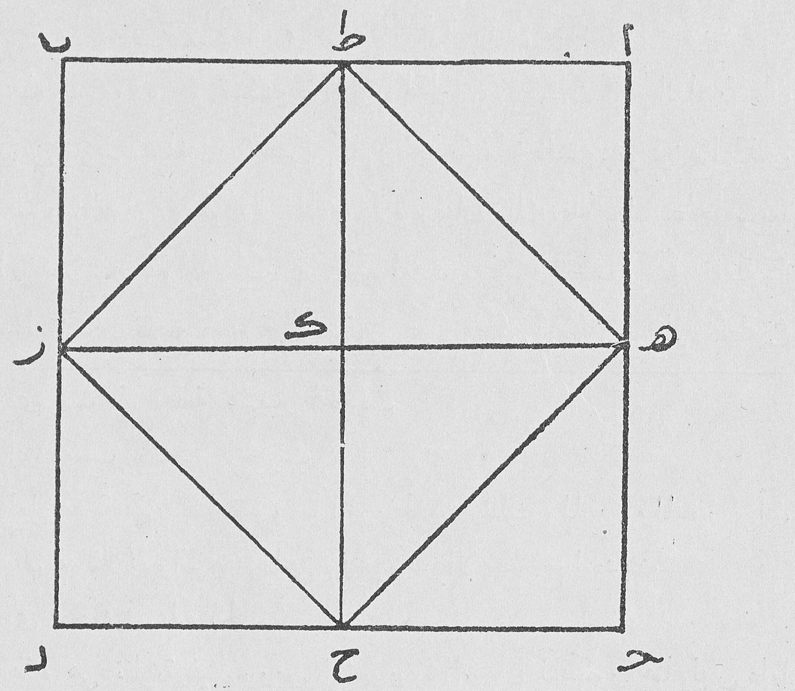
\includegraphics[width=0.6\linewidth,height=0.5\textheight,keepaspectratio]{figures/AK01-F074-FIG1.png}\end{center}\smallskip
\par\smallskip\noindent\rule{30mm}{0.4pt}\Withheld{the editors’ note (\RL{\ArBody ١}), 1 printed line --- not reproduced}
\FrameHead{75}{p. 59}{075}{p. \RL{\ArBody ٥٩}}
\EdL{1}{AK01-F075-L01}{اعلم أن المربعات \NoteMark{١} خمسة أجناس فمنها مستوية الأضلاع قائمة الزوايا والثانية}
\EdL{2}{AK01-F075-L02}{قائمة الزوايا مختلفة الأضلاع طولها أكثر من عرضها . والثالثة تسمى المعينةوهى}
\EdL{3}{AK01-F075-L03}{التى استوت أضلاعها واختلفت زواياها . والرابعة المشبهة بالمعينة وهى التى طولها}
\EdL{4}{AK01-F075-L04}{وعرضها مختلفان وزواياها مختلفة غير أن الطولين متساويان والعرضين}
\EdL{5}{AK01-F075-L05}{متساويان أيضاً . والخامسة المختلفة الاضلاع والزوايا . فما كان من المربعات}
\EdL{6}{AK01-F075-L06}{مستوية الاضلاع قائمة الزوايا أو مختلفة الاضلاع قائمة الزوايا فان تكسيرها}
\EdL{7}{AK01-F075-L07}{أن تضرب الطول فى العرض فما}
\EdL{8}{AK01-F075-L08}{بلغ فهو التكسير . ومثال ذلك}
\EdL{9}{AK01-F075-L09}{أرض مربعة من كل جانب خمسة}
\EdL{10}{AK01-F075-L10}{أذرع تكسيرها خمسة وعشرون}
\EdL{11}{AK01-F075-L11}{ذراعاً وهذه صورتها . والثانية}
\EdL{12}{AK01-F075-L12}{أرض مربعة طولها ثمانية أذرع}
\par\smallskip\begin{center}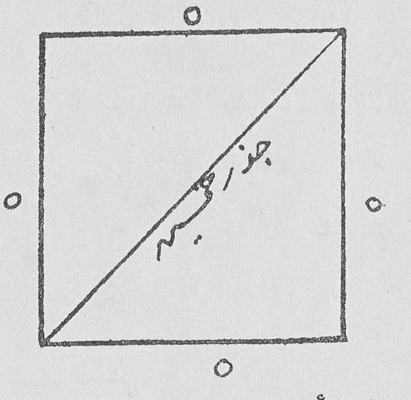
\includegraphics[width=0.6\linewidth,height=0.5\textheight,keepaspectratio]{figures/AK01-F075-FIG1.png}\end{center}\smallskip
\EdL{13}{AK01-F075-L13}{ثمانية أذرع والعرضان ستة}
\EdL{14}{AK01-F075-L14}{ستة . فتكسيرها أن تضرب}
\EdL{15}{AK01-F075-L15}{ستة فى ثمانية فيكون ثمانية}
\EdL{16}{AK01-F075-L16}{وأربعين ذراعاً وذلك}
\EdL{17}{AK01-F075-L17}{تكسيرها وهذه صورتها .}
\EdL{18}{AK01-F075-L18}{وأما المعينة المستوية}
\EdL{19}{AK01-F075-L19}{الأضلاع التى كل جانب منها}
\par\smallskip\begin{center}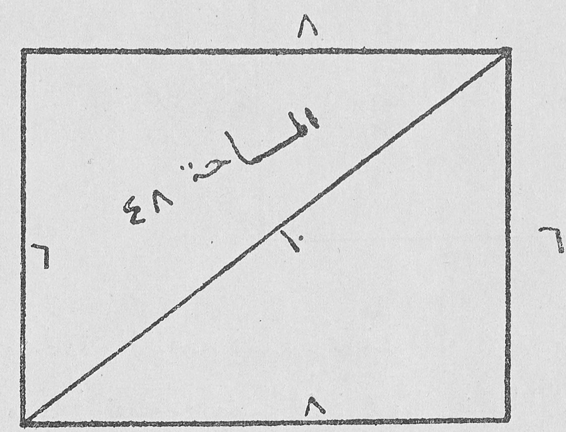
\includegraphics[width=0.6\linewidth,height=0.5\textheight,keepaspectratio]{figures/AK01-F075-FIG2.png}\end{center}\smallskip
\par\smallskip\noindent\rule{30mm}{0.4pt}\Withheld{the editors’ note (\RL{\ArBody ١}), 2 printed lines --- not reproduced}
\FrameHead{76}{p. 60}{076}{p. \RL{\ArBody ٦٠}}
\EdL{1}{AK01-F076-L01}{خمسة أذرع وأحد قطريها ثمانية والآخر ستة أذرع فاعلم أن تكسيرها أن}
\EdL{2}{AK01-F076-L02}{تعرف القطرين أو أحدهما فان عرفت القطرين جميعاً فان الذى يكون}
\EdL{3}{AK01-F076-L03}{من ضرب أحدهما فى نصف الآخر هو تكسيرها وذلك أن تضرب}
\EdL{4}{AK01-F076-L04}{ثمانية فى ثلاثة أو أربعة فى ستة فيكون أربعة}
\EdL{5}{AK01-F076-L05}{وعشرين ذراعاً وهو تكسيرها . فان عرفت}
\EdL{6}{AK01-F076-L06}{قطراً واحدا فقد علمت انهما مثلثتان كل}
\EdL{7}{AK01-F076-L07}{واحدة منهما ضلعاها خمسة أذرع والضلع}
\EdL{8}{AK01-F076-L08}{الثالث هو قطرهما فاحسبها على حساب المثلثات}
\par\smallskip\begin{center}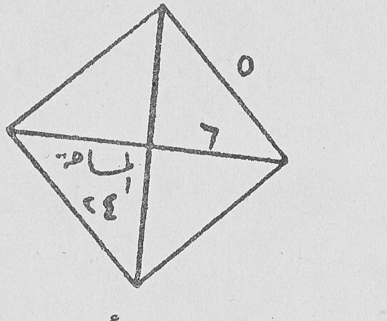
\includegraphics[width=0.6\linewidth,height=0.5\textheight,keepaspectratio]{figures/AK01-F076-FIG1.png}\end{center}\smallskip
\EdL{9}{AK01-F076-L09}{وهذه صورتها . وأما المشبهة بالمعينة فعلى مثال المعينة . وأما سائر المربعات فانما}
\EdL{10}{AK01-F076-L10}{يعرف تكسيرها من قبل القطر فيخرج الى حساب المثلثات فاعلم}
\EdL{11}{AK01-F076-L11}{ذلك وهذه صورة المشبهة بالمعينة . وأما المثلثات فهى ثلاثة أجناس القائمة}
\par\smallskip\begin{center}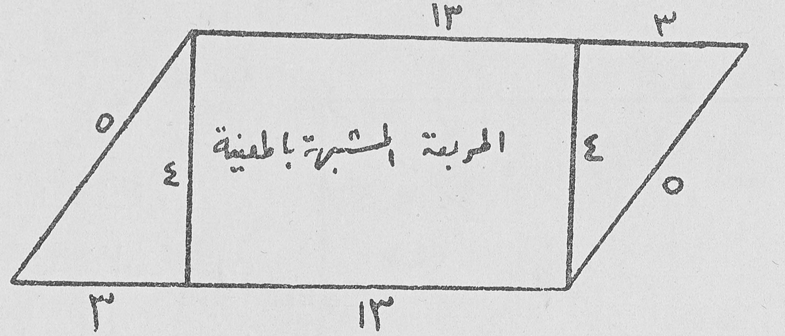
\includegraphics[width=0.6\linewidth,height=0.5\textheight,keepaspectratio]{figures/AK01-F076-FIG2.png}\end{center}\smallskip
\EdL{12}{AK01-F076-L12}{والحادة والمنفرجة. فأما القائمة فهى مثلثة اذا ضربت ضلعيها الأقصرين كل واحد}
\EdL{13}{AK01-F076-L13}{منهما فى نفسه وجمعتهما كان ذلك مثل ضلعها الأطول مضروباً فى نفسه . وأما}
\EdL{14}{AK01-F076-L14}{الحادة فكل مثلثة اذا ضربت ضلعيها الأقصرين كل واحد منهما فى نفسه ثم}
\EdL{15}{AK01-F076-L15}{جمعتهما كانا أكثر من الضلع الأطول مضروباً فى نفسه . وأما المنفرجة فهى}
\FrameHead{77}{p. 61}{077}{p. \RL{\ArBody ٦١}}
\EdL{1}{AK01-F077-L01}{كل مثلثة اذا ضربت ضلعيها الأقصرين كل واحد منهما فى نفسه وجمعتهما كانا}
\EdL{2}{AK01-F077-L02}{أقل من الضلع الأطول مضروبا فى نفسه . فأما القائمة الزوايا فهى التى لها}
\EdL{3}{AK01-F077-L03}{عمودان وقطر وهى نصف مربعة فمعرفة تكسيرها أن تضرب أحد الضلعين}
\EdL{4}{AK01-F077-L04}{المحيطين بالزاوية القائمة فى نصف الآخر فما بلغ ذلك فهو تكسيرها ومثال ذلك}
\EdL{5}{AK01-F077-L05}{مثلثة قائمة الزاوية ضلع منها ستة أذرع وضلع منها ثمانية أذرع والقطر عشرة}
\EdL{6}{AK01-F077-L06}{فحساب ذلك أن تضرب ستة فى أربعة فيكون أربعةوعشرين ذراعا وهو تكسيرها}
\EdL{7}{AK01-F077-L07}{وان أحببت أن تحسبها بالعمود فان عمودها لا يقع إلا على الضلع الأطول لأن}
\EdL{8}{AK01-F077-L08}{الضلعين القصيرين عمودان فان أردت ذلك}
\EdL{9}{AK01-F077-L09}{فاضرب عمودها فى نصف القاعدة فما كان}
\EdL{10}{AK01-F077-L10}{فهو تكسيرها وهذه صورتها . وأما الجنس}
\EdL{11}{AK01-F077-L11}{الثانى فالمثلثة المتساوية الأضلاع حادة}
\EdL{12}{AK01-F077-L12}{الزوايا من كل جانب عشرة أذرع فان}
\par\smallskip\begin{center}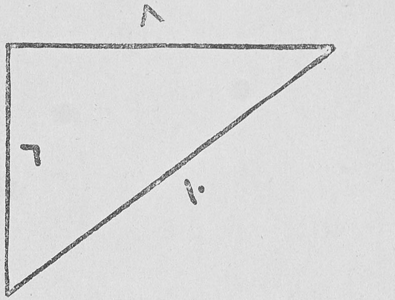
\includegraphics[width=0.6\linewidth,height=0.5\textheight,keepaspectratio]{figures/AK01-F077-FIG1.png}\end{center}\smallskip
\EdL{13}{AK01-F077-L13}{تكسيرها يعرف من قبل عمودها ومسقط حجرها واعلم أن كل ضلعين مستويين}
\EdL{14}{AK01-F077-L14}{من مثلثةيخرج بينهما عمود على قاعدة فان مسقط حجر العمود يقع على زاوية قائمة}
\EdL{15}{AK01-F077-L15}{ويقع على نصف القاعدةسواءاذا استوى الضلعان.فان اختلفا خالف مسقط الحجر}
\EdL{16}{AK01-F077-L16}{عن نصف القاعدة ولكن قد علمنا أن مسقط حجر هذه المثلثة على أى أضلاعها}
\EdL{17}{AK01-F077-L17}{جعلته لا يقع إلا على نصفه فذلك خمسة أذرع فمعرفة العمود أن تضرب الخمسة}
\EdL{18}{AK01-F077-L18}{فى مثلها وتضرب أحد الضلعين فى مثله وهو عشرة فيكون مائة فتنقص}
\EdL{19}{AK01-F077-L19}{منها مبلغ الخمسة فى مثلها وهو خمسة وعشرون فيبقى خمسة وسبعون فخذ}
\EdL{20}{AK01-F077-L20}{جذر ذلك فهو العمود وقد صار ضلعا على مثلثتين قائمتين فان أردت}
\EdL{21}{AK01-F077-L21}{التكسير فاضرب جذر الخمسة والسبعين فى نصف القاعدة وهو خمسة وذلك}
\FrameHead{78}{p. 62}{078}{p. \RL{\ArBody ٦٢}}
\EdL{1}{AK01-F078-L01}{أن تضرب الخمسة فى مثلها حتى يكون جذر خمسة وسبعون فى جذر خمسة}
\EdL{2}{AK01-F078-L02}{وعشرين فاضرب خمسة وسبعين فى خمسة وعشرين فيكون ألفا وثمانى مائة}
\EdL{3}{AK01-F078-L03}{وخمسة وسبعين فخذ جذر ذلك فهو}
\EdL{4}{AK01-F078-L04}{تكسيرها وهو ثلاثة وأربعون وشىء}
\EdL{5}{AK01-F078-L05}{قليل وهذه صورتها . وقد تكون من}
\EdL{6}{AK01-F078-L06}{هذه الزوايا الحادة مختلفة الأضلاع فاعلم}
\EdL{7}{AK01-F078-L07}{أن تكسيرها يعلم من قبل مسقط حجرها}
\EdL{8}{AK01-F078-L08}{وعمودها وهى أن تكون مثلثة من جانب}
\par\smallskip\begin{center}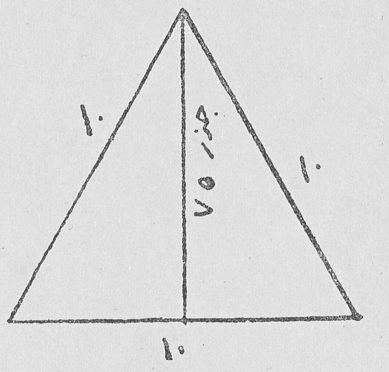
\includegraphics[width=0.6\linewidth,height=0.5\textheight,keepaspectratio]{figures/AK01-F078-FIG1.png}\end{center}\smallskip
\EdL{9}{AK01-F078-L09}{خمسة عشر ذراعا ومن جانب أربعة عشر ذراعا ومن جانب ثلاثة عشر ذراعا}
\EdL{10}{AK01-F078-L10}{فاذا أردت علم مسقط حجرها فاجعل القاعدة أى الجوانب شئت فجعلناها أربعة}
\EdL{11}{AK01-F078-L11}{عشر وهو مسقط الحجر فمسقط حجرها يقع منها على شىء مما يلى أى الضلعين}
\EdL{12}{AK01-F078-L12}{شئت فجعلنا الشىء مما يلى الثلاثة عشر فضربناه فى مثله فصار مالا ونقصناه}
\EdL{13}{AK01-F078-L13}{من ثلاثة عشر فى مثلها وهو مائة وتسعة وستون فصار ذلك مائة وتسعة وستين}
\EdL{14}{AK01-F078-L14}{الا مالا فعلمنا أن جذرها هو العمود وقد بقى لنا من القاعدة أربعة عشر الا}
\EdL{15}{AK01-F078-L15}{شيئا فضربناه فى مثله فصار مائة وستة وتسعين ومالا الا ثمانية وعشرين}
\EdL{16}{AK01-F078-L16}{شيئا فنقصناه من الخمسة عشر فى مثلها فبقى تسعة وعشرون (درهما \NoteMark{١}) وثمانية}
\EdL{17}{AK01-F078-L17}{وعشرون شيئا الا مالا وجذرها هو العمود فلما صارجذرها هذا هو العمود وجذر}
\EdL{18}{AK01-F078-L18}{مائة وتسعة وستين الا مالا هو العمود أيضا علمنا أنهما متساويان فقابل بينهما}
\par\smallskip\noindent\rule{30mm}{0.4pt}\Withheld{the editors’ note (\RL{\ArBody ١}), 1 printed line --- not reproduced}
\FrameHead{79}{p. 63}{079}{p. \RL{\ArBody ٦٣}}
\EdL{1}{AK01-F079-L01}{وهو أن تلقى مالا بمال لأن المالين ناقصان فيبقى تسعة وعشرون وثمانية}
\EdL{2}{AK01-F079-L02}{وعشرون شيئا تعدل مائة وتسعة وستين . فالق تسعة وعشرين من مائة وتسعة}
\EdL{3}{AK01-F079-L03}{وستين فيبقى مائة وأربعون تعدل ثمانية وعشرين شيئا فالشىء الواحد خمسة}
\EdL{4}{AK01-F079-L04}{وهو مسقط الحجر مما يلى الثلاثة عشر وتمام القاعدة مما يلى الضلع الآخر فهو}
\EdL{5}{AK01-F079-L05}{تسعة فاذا أردت أن تعرف العمود فاضرب هذه الخمسة فى مثلها وانقصها من}
\EdL{6}{AK01-F079-L06}{الضلع الذى يليها مضروبا فى مثله وهو ثلاثة عشر فيبقى مائة وأربعة وأربعون}
\EdL{7}{AK01-F079-L07}{فجذر ذلك هو العمود وهو اثنى عشر والعمود أبدا يقع على القاعدة على زاويتين}
\EdL{8}{AK01-F079-L08}{قائمتين ولذلك سمى عمودا لأنه مستو فاضرب العمود فى نصف القاعدة وهو}
\EdL{9}{AK01-F079-L09}{سبعة فيكون اربعة}
\EdL{10}{AK01-F079-L10}{وثمانين وذلك تكسيرها}
\EdL{11}{AK01-F079-L11}{وهذه صورتها .}
\EdL{12}{AK01-F079-L12}{\Bd{والجنس الثالث} المنفرجة}
\EdL{13}{AK01-F079-L13}{وهى التى لها زاوية}
\EdL{14}{AK01-F079-L14}{منفرجة وهى مثلثة من}
\EdL{15}{AK01-F079-L15}{كل جانب عدد مختلف}
\par\smallskip\begin{center}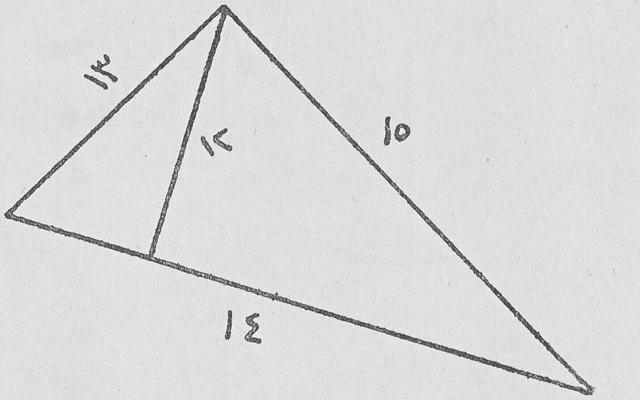
\includegraphics[width=0.6\linewidth,height=0.5\textheight,keepaspectratio]{figures/AK01-F079-FIG1.png}\end{center}\smallskip
\EdL{16}{AK01-F079-L16}{وهى من جانب ستة ومن جانب خمسة ومن جانب تسعة فمعرفة تكسير هذه من}
\EdL{17}{AK01-F079-L17}{قبل عمودها ومسقط حجرها ولا يقع مسقط هذه المثلثة فى جوفها الا على الضلع}
\EdL{18}{AK01-F079-L18}{الأطول فاجعله قاعدة ولوجعلت أحد الضلعين الأقصرين قاعدة لوقع مسقط حجرها}
\EdL{19}{AK01-F079-L19}{خارجها وعلم مسقط حجرها وعمودها على مثال ماعملت لك فى الحادة وعلى ذلك}
\EdL{20}{AK01-F079-L20}{القياس وهذه صورتها . وأما المدورات التى فرغنا من صفتها وتكسيرها فى}
\FrameHead{80}{p. 64}{080}{p. \RL{\ArBody ٦٤}}
\EdL{1}{AK01-F080-L01}{صدر الكتاب فمنها مدورة}
\EdL{2}{AK01-F080-L02}{قطرها سبعة أذرع ويحيط}
\EdL{3}{AK01-F080-L03}{بها اثنان وعشرون ذراعا \NoteMark{١}}
\EdL{4}{AK01-F080-L04}{فان تكسيرها أن تضرب}
\EdL{5}{AK01-F080-L05}{نصف القطر وهو ثلاثة ونصف}
\par\smallskip\begin{center}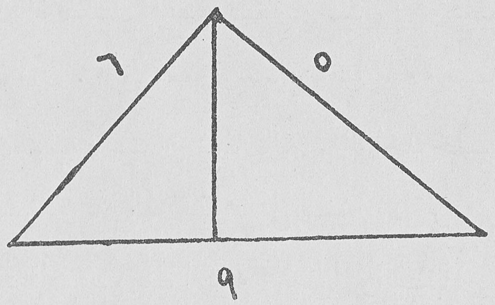
\includegraphics[width=0.6\linewidth,height=0.5\textheight,keepaspectratio]{figures/AK01-F080-FIG1.png}\end{center}\smallskip
\EdL{6}{AK01-F080-L06}{فى نصف الدور الذى يحيط بها وهو أحد عشر فيكون ثمانية وثلاثين ونصفا}
\EdL{7}{AK01-F080-L07}{وهو تكسيرها فان أحببت فاضرب القطر وهو سبعة فى مثله فيكون تسعة}
\EdL{8}{AK01-F080-L08}{وأربعين فانقص منها سبعها ونصف سبعها}
\EdL{9}{AK01-F080-L09}{وهو عشرة ونصف فيبقى ثمانية وثلاثون}
\EdL{10}{AK01-F080-L10}{ونصف وهو التكسير وهذه صورتها .}
\EdL{11}{AK01-F080-L11}{فان قال عمود مخروط أسفله أربعة}
\EdL{12}{AK01-F080-L12}{أذرع فى أربعة أذرع وارتفاعه عشرة}
\EdL{13}{AK01-F080-L13}{أذرع ورأسه ذراعان فى ذراعين .}
\par\smallskip\begin{center}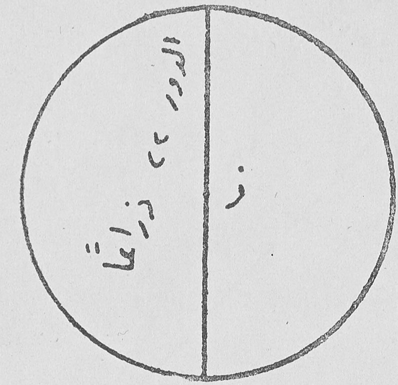
\includegraphics[width=0.6\linewidth,height=0.5\textheight,keepaspectratio]{figures/AK01-F080-FIG2.png}\end{center}\smallskip
\EdL{14}{AK01-F080-L14}{وقد كنا بينا أن كل مخروط محدد الرأس فان ثلث تكسير أسفله مضروبا}
\EdL{15}{AK01-F080-L15}{فى عموده هو تكسيره فلما صار هذا غير محدد أردنا أن نعلم كم يرتفع حتى يفنى}
\EdL{16}{AK01-F080-L16}{رأسه فيكون لا رأس له فعلمنا أن هذه العشرة من الطول كله كقدر الاثنين}
\EdL{17}{AK01-F080-L17}{من الأربعة فالاثنان نصف الأربعةفاذا كان ذلك كذلك فالعشرة نصف الطول}
\par\smallskip\noindent\rule{30mm}{0.4pt}\Withheld{the editors’ note (\RL{\ArBody ١}), 3 printed lines --- not reproduced}
\FrameHead{81}{p. 65}{081}{p. \RL{\ArBody ٦٥}}
\EdL{1}{AK01-F081-L01}{والطول كله عشرون ذراعا فلما عرفنا الطول أخذنا ثلث تكسير الأسفل}
\EdL{2}{AK01-F081-L02}{وهو خمسة وثلث فضربناه فى الطول وهو عشرون ذراعا فبلغ ذلك مائة وستة}
\EdL{3}{AK01-F081-L03}{أذرع وثلثى ذراع فأردنا أن نلقى منه ما زدنا عليه حتى انخرط وهو واحد وثلث}
\EdL{4}{AK01-F081-L04}{الذى هو ثلث تكسير اثنين فى اثنين فى عشرة وهو ثلاثة عشر وثلث وذلك}
\EdL{5}{AK01-F081-L05}{تكسير ما زدنا عليه حتى انخرط فاذا رفعنا ذلك من مائة وستة أذرع وثلثى}
\EdL{6}{AK01-F081-L06}{ذراع بقى ثلاثة وتسعون ذراعا وثلث}
\EdL{7}{AK01-F081-L07}{وذلك تكسير العمود المخروط وهذه}
\EdL{8}{AK01-F081-L08}{صورته . وان كان المخروط مدورا فالق}
\EdL{9}{AK01-F081-L09}{من ضرب قطره فى نفسه سبعه ونصف}
\EdL{10}{AK01-F081-L10}{سبعه فما بقى فهو تكسيره \NoteMark{١} . فان قيل}
\EdL{11}{AK01-F081-L11}{أرض مثلثة من جانبيها عشرة أذرع عشرة}
\EdL{12}{AK01-F081-L12}{أذرع والقاعدة اثنا عشر ذراعا فى جوفها}
\EdL{13}{AK01-F081-L13}{أرض مربعة كم كل جانب من المربعة فقياس}
\par\smallskip\begin{center}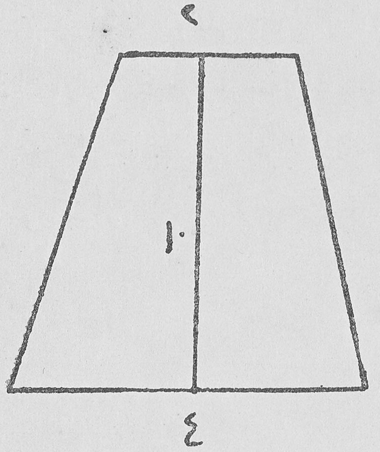
\includegraphics[width=0.6\linewidth,height=0.5\textheight,keepaspectratio]{figures/AK01-F081-FIG1.png}\end{center}\smallskip
\EdL{14}{AK01-F081-L14}{ذلك أن تعرف عمود المثلثة وهو أن تضرب نصف القاعدة وهو ستة فى مثله فيكون}
\EdL{15}{AK01-F081-L15}{ستة وثلاثين فانقصها من أحد الجانبين الأقصرين مضروباً فى مثله وهو مائة}
\EdL{16}{AK01-F081-L16}{يبقى أربعة وستون فخذ جذرها ثمانية وهو العمود وتكسيرها ثمانية وأربعون}
\EdL{17}{AK01-F081-L17}{ذراعاً وهو ضربك العمود فى نصف القاعدة وهو ستة فجعلنا أحد جوانب}
\EdL{18}{AK01-F081-L18}{المربعة شيئا وضربناه فى مثله فصار مالا فحفظناه ثم علمنا أنه قد بقى لنا مثلثتان}
\EdL{19}{AK01-F081-L19}{عن جنبتى المربعة ومثلثة فوقها فأما المثلثتان اللتان على جنبتى المربعة فهما متساويتان}
\EdL{20}{AK01-F081-L20}{وعموداهما واحد وهما على زاوية قائمة فتكسيرها أن تضرب شيئاً فى ستة الا}
\par\smallskip\noindent\rule{30mm}{0.4pt}\Withheld{the editors’ note (\RL{\ArBody ١}), 1 printed line --- not reproduced}
\FrameHead{82}{p. 66}{082}{p. \RL{\ArBody ٦٦}}
\EdL{1}{AK01-F082-L01}{نصف شىء فيكون ستة أشياء إلا نصف مال وهو تكسير المثلثتين جميعاً اللتين}
\EdL{2}{AK01-F082-L02}{هما على جنبتى المربعة . فأما تكسير المثلثة العليا فهو أن تضرب ثمانية غير شىء}
\EdL{3}{AK01-F082-L03}{وهو العمود فى نصف شىء فيكون أربعة أشياء إلا نصف مال فهذا هو تكسير}
\EdL{4}{AK01-F082-L04}{المربعة وتكسير الثلاث مثلثات وهو}
\EdL{5}{AK01-F082-L05}{عشرة أشياء تعدل ثمانية وأربعين هو}
\EdL{6}{AK01-F082-L06}{تكسير المثلثة العظمى فالشىء الواحد من}
\EdL{7}{AK01-F082-L07}{ذلك أربعة أذرع واربعة أخماس ذراع}
\EdL{8}{AK01-F082-L08}{وهو كل جانب من المربعة وهذه}
\EdL{9}{AK01-F082-L09}{صورتها .}
\par\smallskip\begin{center}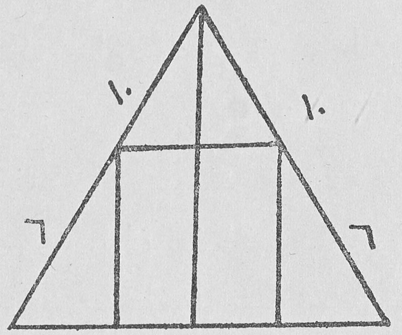
\includegraphics[width=0.6\linewidth,height=0.5\textheight,keepaspectratio]{figures/AK01-F082-FIG1.png}\end{center}\smallskip
\FrameHead{83}{p. [67]}{083}{p. [\RL{\ArBody ٦٧}]}
\EdLh{1}{AK01-F083-L01}{كتاب الوصايا}
\EdLp{2}{AK01-F083-L02}{\Bd{باب من ذلك فى العين والدين} رجل مات وترك ابنين وأوصى بثلث ماله}
\EdL{3}{AK01-F083-L03}{لرجل أجنبى وترك عشرة دراهم عينا وعشرة دراهم دينا على أحد الابنين \NoteMark{١} .}
\EdL{4}{AK01-F083-L04}{قياسه أن تجعل المستخرج من الدين شيئاً فتزيده على العين وهو عشرة دراهم}
\EdL{5}{AK01-F083-L05}{فيكون عشرة وشيئاً ثم تعزل ثلثها لأنه أوصى بثلث ماله وهو ثلاثة دراهم وثلث}
\EdL{6}{AK01-F083-L06}{وثلث شىء فيبقى ستة دراهم وثلثان وثلثا شىء فتقسمه بين الابنين فيصيب كل}
\EdL{7}{AK01-F083-L07}{ابن ثلاثة دراهم وثلث درهم وثلث شىء فهو يعدل الشىء المستخرج فقابل به}
\EdL{8}{AK01-F083-L08}{فتلقى ثلثاً من شىء بثلث شىء فيبقى ثلثا شىء تعدل ثلاثة دراهم وثلثا فتحتاج أن}
\EdL{9}{AK01-F083-L09}{تكمل الشىء الذى استخرج من الدين . فان ترك ابنين وترك عشرة دراهم عينا}
\EdL{10}{AK01-F083-L10}{وعشرة دراهم ديناعلى أحد الابنين وأوصى لرجل بخمس ماله ودرهم \NoteMark{٢}فقياسه}
\EdL{11}{AK01-F083-L11}{أن تجعل ما يستخرج من الدين شيئاً فتزيده على العين فتكون شيئاً وعشرةدراهم}
\EdL{12}{AK01-F083-L12}{فتعزل خمسها لأنه أوصى بخمس ماله وهو درهمان وخمس شىء فيبقى ثمانيةدراهم}
\par\smallskip\noindent\rule{30mm}{0.4pt}\Withheld{the editors’ notes (\RL{\ArBody ١}) (\RL{\ArBody ٢}), 8 printed lines --- not reproduced}
\FrameHead{84}{p. 68}{084}{p. \RL{\ArBody ٦٨}}
\EdL{1}{AK01-F084-L01}{وأربعة أخماس شىء ثم تعزل الدرهم الذى أوصى به فيبقى سبعة دراهم وأربعة}
\EdL{2}{AK01-F084-L02}{أخماس شىء فتقسمه بين الاثنين فيكون لكل واحد ثلاثة دراهم ونصف درهم}
\EdL{3}{AK01-F084-L03}{وخمسا شىء تعدل شيئاً فتلقى خمسى شىء من شىء فيبقى ثلاثة أخماس شىء تعدل}
\EdL{4}{AK01-F084-L04}{ثلاثة دراهم ونصفا فكمل الشىء وهو أن تزيد عليه مثل ثلثيه وتزيد على الثلاثة}
\EdL{5}{AK01-F084-L05}{والنصف مثل ثلثيها وهو درهمان وثلث فتكون خمسة دراهم وخمسة أسداس}
\EdL{6}{AK01-F084-L06}{وهو الشىء الذى استخرج من الدين . فان ترك ثلاثة بنين وأوصى بخمس ماله}
\EdL{7}{AK01-F084-L07}{إلا درهماً وترك عشرة دراهم عينا وعشرة دراهم دينا على أحد البنين \NoteMark{١} فان}
\EdL{8}{AK01-F084-L08}{قياسه أن تجعل الذى يستخرج من الدين شيئاً فتزيده على العشرة فيكون عشرة}
\EdL{9}{AK01-F084-L09}{وشيئاً فتعزل خمسها للوصيةوهو درهمان وخمس شىء فيبقى ثمانية دراهم وأربعة}
\EdL{10}{AK01-F084-L10}{أخماس شىء ثم تستثنى درهما لأنه قال إلا درهماً فيكون تسعة دراهم وأربعة}
\EdL{11}{AK01-F084-L11}{أخماس شىء فتقسم ذلك بين البنين فيكون لكل ابن ثلاثة دراهم وخمس شىء}
\EdL{12}{AK01-F084-L12}{وثلث خمس شىء فيكون ذلك يعدل شيئاً فتلقى خمس شىء وثلث خمس شىء}
\EdL{13}{AK01-F084-L13}{من شىء فيبقى أحد عشر جزءاً من خمسة عشر جزءاً من شىء تعدل ثلاثة دراهم}
\EdL{14}{AK01-F084-L14}{فتحتاج الى أن تكمل الشىء فتزيد عليه أربعة أجزاء من أحد عشر من شىءوتزيد}
\EdL{15}{AK01-F084-L15}{مثل ذلك على ثلاثة دراهم وهو درهم وجزء من أحد عشر جزءاً فيكون أربعة}
\EdL{16}{AK01-F084-L16}{دراهم وجزءاً من أحد عشر جزءاً من درهم تعدل شيئاً وهو الذى استخرج من}
\EdL{17}{AK01-F084-L17}{الدين . \Bd{باب آخر من الوصايا} . رجل مات وترك أمه وامرأته وأخاه وأختيه}
\par\smallskip\noindent\rule{30mm}{0.4pt}\Withheld{the editors’ note (\RL{\ArBody ١}), 4 printed lines --- not reproduced}
\FrameHead{85}{p. 69}{085}{p. \RL{\ArBody ٦٩}}
\EdL{1}{AK01-F085-L01}{لأبيه وأمه وأوصى لرجل بتسع ماله \NoteMark{١} فان قياس ذلك أن تقيم فريضتهم فتجدها}
\EdL{2}{AK01-F085-L02}{من ثمانية وأربعين سهماً فأنت تعلم أن كل مال نزعت تسعه بقيت ثمانية أتساعه}
\EdL{3}{AK01-F085-L03}{وان الذى نزعت مثل ثمن ما أبقيت فتزيد على الثمانية الأتساع ثمنها وعلى الثمانية}
\EdL{4}{AK01-F085-L04}{والأربعين مثل ثمنها ليتم مالك وهو ستة فيكون ذلك أربعة وخمسين للموصى}
\EdL{5}{AK01-F085-L05}{له بالتسع من ذلك ستة وهو تسع جميع المال وما بقى فهو ثمانية وأربعون بين}
\EdL{6}{AK01-F085-L06}{الورثة على سهامهم . \Bd{فان قال} امرأة ملكت وتركت زوجها وابنها وثلاث}
\EdL{7}{AK01-F085-L07}{بنات وأوصت لرجل بثمن مالها وسبعه \NoteMark{٢} فاقم سهام الورثة (الفريضة) فتجدها}
\EdL{8}{AK01-F085-L08}{من عشرين وخذ مالا فالق ثمنه وسبعه فيبقى مال الا ثمنا وسبعا فتمم مالك وهو}
\EdL{9}{AK01-F085-L09}{أن تزيد عليه خمسة عشر جزءاً من أحد وأربعين جزءاً فاضرب سهام الفريضة}
\EdL{10}{AK01-F085-L10}{وهى عشرون فى أحد وأربعين فيكون ثمانى مائة وعشرين فتزيد على ذلك خمسة}
\EdL{11}{AK01-F085-L11}{عشر جزءاً من أحد وأربعين وهو ثلاثمائة جزء فيصير ذلك كله ألفاً ومائة}
\EdL{12}{AK01-F085-L12}{وعشرين سهما للموصى له من ذلك بالثمن والسبع سبع ذلك وثمنه وهو ثلاثمائة .}
\par\smallskip\noindent\rule{30mm}{0.4pt}\Withheld{the editors’ notes (\RL{\ArBody ١}) (\RL{\ArBody ٢}), 9 printed lines --- not reproduced}
\FrameHead{86}{p. 70}{086}{p. \RL{\ArBody ٧٠}}
\EdL{1}{AK01-F086-L01}{السبع مائة وستون والثمن مائة وأربعون وبقى ثمانمائة وعشرون سهما بين}
\EdL{2}{AK01-F086-L02}{الورثة على سهامهم . \Bd{باب آخر من الوصايا} وهو اذا لم يجز بعض الورثة وأجاز}
\EdL{3}{AK01-F086-L03}{بعضهم والوصية أكثر من الثلث . اعلم أن الحكم فى ذلك أن من أجاز من الورثة}
\EdL{4}{AK01-F086-L04}{أكثر من الثلث من الوصية فذلك داخل عليه فى حصته ومن لم يجز فالثلث}
\EdL{5}{AK01-F086-L05}{جايز عليه على كل حال . \Bd{مثال ذلك} إمرة ماتت وتركث زوجها وابنها وامها}
\EdL{6}{AK01-F086-L06}{وأوصت لرجل بخمسى مالها ولآخر بربع مالها فأجاز الابن الوصيتين جميعاً}
\EdL{7}{AK01-F086-L07}{وأجازت الأم النصف لهما ولم يجز الزوج شيئاً من ذلك الا الثلث \NoteMark{١} فقياس}
\EdL{8}{AK01-F086-L08}{ذلك أن تقيم سهام الفريضة فتجدها من اثنى عشر سهما . للابن من ذلك سبعة}
\EdL{9}{AK01-F086-L09}{أسهم وللزوج ثلاثة أسهم وللأم سهمان وأنت تعلم أن الزوج يجوز عليه الثلث}
\EdL{10}{AK01-F086-L10}{فينبغى أن يكون فى يده مثلا ما يخرج من حصته للوصايا وفى يده ثلاثة للوصايا}
\par\smallskip\noindent\rule{30mm}{0.4pt}\Withheld{the editors’ note (\RL{\ArBody ١}), 12 printed lines --- not reproduced}
\FrameHead{87}{p. 71}{087}{p. \RL{\ArBody ٧١}}
\EdL{1}{AK01-F087-L01}{سهم وله سهمان . وأما الابن الذى أجاز الوصيتين جميعاً فينبغى أن يؤخذ منه}
\EdL{2}{AK01-F087-L02}{خمسا جميع ماله وربعه فيبقى فى يده سبعة أسهم من عشرين سهما والذى له كله}
\EdL{3}{AK01-F087-L03}{عشرون سهما . وأما الأم فينبغى أن يبقى فى يدها مثل ما يخرج من يدها وهو}
\EdL{4}{AK01-F087-L04}{واحد وجميع ما كان لها اثنان . فخذ مالا يكون لربعه ثلث ولسدسه نصف}
\EdL{5}{AK01-F087-L05}{ويكون مايبقى ينقسم بين عشرين فذلك مائتان واربعون . للأم من ذلك السدس}
\EdL{6}{AK01-F087-L06}{وهو اربعون الوصية من ذلك عشرون ولها عشرون . وللزوج من ذلك الربع}
\EdL{7}{AK01-F087-L07}{ستون الوصية من ذلك عشرون وله اربعون . ويبقى مائة واربعون للابن. الوصية}
\EdL{8}{AK01-F087-L08}{من ذلك خمساه وربعه وهو واحد وتسعون وتبقى تسعة واربعون فجميع الوصية}
\EdL{9}{AK01-F087-L09}{مائة وأحد وثلاثون بين الرجلين الموصى لهما لصاحب الخمسين من ذلك ثمانية}
\EdL{10}{AK01-F087-L10}{أجزاء من ثلاثة عشر جزءاً ولصاحب الربع خمسة أجزاء من ثلاثةعشر جزءاً فان}
\EdL{11}{AK01-F087-L11}{أردت أن تصحح سهام الرجلين الموصى لهما فاضرب سهام الفريضة فى ثلاثة عشر}
\EdL{12}{AK01-F087-L12}{يصبح من ثلاثة آلاف ومائة وعشرين . \Bd{فان أجاز} الابن الخمسين لصاحب}
\EdL{13}{AK01-F087-L13}{الخمسين ولم يجز للآخر شيئا وأجازت الأم الربع لصاحب الربع ولم تجز للآخر}
\EdL{14}{AK01-F087-L14}{شيئا ولم يجز الزوج لهما الا الثلث فاعلم أن الثلث للرجلين جائز على جميع الورثة}
\EdL{15}{AK01-F087-L15}{يضرب فيه صاحب الخمسين بثمانية أجزاء من ثلاثة عشر جزءاً وصاحب الربع}
\EdL{16}{AK01-F087-L16}{بخمسة أجزاء من ثلاثة عشر فأقم الفريضة على ما ذكرت لك فيكون اثنى عشر}
\EdL{17}{AK01-F087-L17}{للزوج الربع وللأم السدس وللابن ما بقى . وقياسه انك تعلم أن الزوج يخرج}
\EdL{18}{AK01-F087-L18}{من يده ثلث حصته على كل حال فينبغى أن يكون فى يده ثلاثة اسهم وأن الأم}
\EdL{19}{AK01-F087-L19}{يخرج من يدها الثلث لكل واحد بقدر حصته فهى اذا أجازت لصاحب الربع}
\EdL{20}{AK01-F087-L20}{من خاصة حصتها فضل ما بين الربع وحصته من نصيبها \NoteMark{١} وهى تسعة عشر}
\par\smallskip\noindent\rule{30mm}{0.4pt}\Withheld{the editors’ note (\RL{\ArBody ١}), 3 printed lines --- not reproduced}
\FrameHead{88}{p. 72}{088}{p. \RL{\ArBody ٧٢}}
\EdL{1}{AK01-F088-L01}{جزءاً من مائة وستة وخمسين من جميع نصيبها فينبغى أن يكون نصيبها مائة وستة}
\EdL{2}{AK01-F088-L02}{وخمسين فحصته من الثلث من نصيبها عشرون سهما والذى أجازت له ربع حصتها}
\EdL{3}{AK01-F088-L03}{وهو تسعة وثلاثون فيؤخذ ثلث مافى يدها لهما وتسعة عشر سهما للذى أجازت}
\EdL{4}{AK01-F088-L04}{له خاصة. ثم الابن قدأجاز لصاحب الخمسين فضل مابين خمسى نصيبه وبين ما يصيبه}
\EdL{5}{AK01-F088-L05}{من الثلث \NoteMark{١} وهو ثمانية وثلاثون من مائة وخمسة وتسعين من نصيب الابن}
\EdL{6}{AK01-F088-L06}{بعد اخراج الثلث لهما لأن الذى له من خاصة الثلث ثمانية أجزاء من ثلاثة عشر}
\EdL{7}{AK01-F088-L07}{من الثلث وهو أربعون . والذى أجازله من خمسى نصيبه ثمانية وثلاثون فذلك}
\EdL{8}{AK01-F088-L08}{ثمانية وسبعون فيؤخذ منه خمسة وستون ثلث ماله لهما والذى أجاز له خاصة ثمانية}
\EdL{9}{AK01-F088-L09}{وثلاثون . فان أردت أن تصحح سهام الفريضة صححتها فكانت من مائتى ألف}
\par\smallskip\noindent\rule{30mm}{0.4pt}\Withheld{the editors’ note (\RL{\ArBody ١}), 13 printed lines --- not reproduced}
\FrameHead{89}{p. 73}{089}{p. \RL{\ArBody ٧٣}}
\EdL{1}{AK01-F089-L01}{وتسعة عشر الفاً وثلاثمائة وعشرين . \Bd{وفى وجه آخر من الوصايا} رجل مات وترك}
\EdL{2}{AK01-F089-L02}{أربعة بنين وامرأة وأوصى لرجل بمثل نصيب أحد البنين الا مثل نصيب المرأة}
\EdL{3}{AK01-F089-L03}{فأقم سهام الفريضة وهى اثنان وثلاثون سهما للمرأة الثمن أربعة ولكل ابن}
\EdL{4}{AK01-F089-L04}{سبعةفأنت تعلم أن الذى أوصى به ثلاثة أسباع نصيب ابن وهو ثلاثة وهى الوصية}
\EdL{5}{AK01-F089-L05}{فيكون ذلك خمسةوثلاثين للموصى له ثلاثة أسهم من خمسةوثلاثين سهماًويبقى}
\EdL{6}{AK01-F089-L06}{اثنان وثلاثون بين الورثة على سهامهم . فان ترك ابنين وبنتاً وأوصى لرجل بمثل}
\EdL{7}{AK01-F089-L07}{نصيب ابن ثالث لو كان . فالوجه فى ذلك أن تنظر الى ابن لو كان البنون ثلاثة}
\EdL{8}{AK01-F089-L08}{كم كانت تكون سهامهم فتجد ذلك سبعة فخذ فريضة يكون لخمسها سبع ولسبعها}
\EdL{9}{AK01-F089-L09}{خمس وذلك خمسة وثلاثون فزد عليها سبعيها وهو عشرة فيكون ذلك خمسة}
\EdL{10}{AK01-F089-L10}{وأربعين للموصى له من ذلك عشرة ولكل ابن أربعة عشر وللبنت سبعة. \Bd{فان ترك}}
\EdL{11}{AK01-F089-L11}{أما وثلاثة بنين وبنتا وأوصى لرجل بمثل نصيب أحد بنيه الا مثل نصيب بنت}
\EdL{12}{AK01-F089-L12}{أخرى لو كانت \NoteMark{١} فأقم سهام الفريضة واجعلها شيئاً ينقسم بين هؤلاء الورثة}
\EdL{13}{AK01-F089-L13}{وبينهم لوكانت معهم ابنة أخرى فتجدها ثلثمائةوستةوثلاثين . فنصيب ابنة لوكانت}
\EdL{14}{AK01-F089-L14}{خمسة وثلاثون ونصيب ابن ثمانون سهما وبينهماخمسة وأربعون وهى الوصية}
\EdL{15}{AK01-F089-L15}{فزدها على ثلاثمائة وستة وثلاثين فيكون ذلك ثلاثمائة واحدا وثمانين فذلك}
\EdL{16}{AK01-F089-L16}{سهام المال . \Bd{فان ترك} ثلاثة بنين وأوصى لرجل بمثل نصيب أحد بنيه الا مثل}
\par\smallskip\noindent\rule{30mm}{0.4pt}\Withheld{the editors’ note (\RL{\ArBody ١}), 5 printed lines --- not reproduced}
\FrameHead{90}{p. 74}{090}{p. \RL{\ArBody ٧٤}}
\EdL{1}{AK01-F090-L01}{نصيب ابنة لو كانت وبثلث ما بقى من الثلث \NoteMark{١} . فقياس ذلك أن تقيم سهام}
\EdL{2}{AK01-F090-L02}{الفريضة على شىء يستقيم بين هؤلاء الورثة وبينهم لو كانت معهم ابنة أخرى}
\EdL{3}{AK01-F090-L03}{فيكون ذلك واحداً وعشرين فلو كانت معهم بنت أخرى لكان لها ثلاثة ونصيب}
\EdL{4}{AK01-F090-L04}{ابن سبعة فقد أوصى له بأربعة أسباع نصيب ابن وثلث ما بقى من الثلث فخذ}
\EdL{5}{AK01-F090-L05}{ثلثاً فاطرح منه أربعة أسباع نصيب ابن فيبقى ثلث مال الا أربعة أسباع نصيب}
\EdL{6}{AK01-F090-L06}{ابن ثم الق ثلث مابقى من الثلث وهوتسع مال الاسبع نصيب وثلث سبع نصيب}
\EdL{7}{AK01-F090-L07}{فيبقى تسع مال الا سبعى نصيب وثلثى سبع نصيب فزد ذلك على ثلثى المال فيكون}
\EdL{8}{AK01-F090-L08}{ثمانية اتساع مال الاسبعى نصيب وثلثى سبع نصيب وذلك ثمانية اجزاء من واحد}
\EdL{9}{AK01-F090-L09}{وعشرين جزءاً من نصيب يعدل ثلاثة انصباء فاجبر ذلك فيكون ثمانية أتساع}
\EdL{10}{AK01-F090-L10}{مال تعدل ثلاثة انصباء وثمانية اجزاء من احد وعشرين جزءاً من نصيب فتمم}
\EdL{11}{AK01-F090-L11}{مالك وهو أن تزيد على الثمانية الاتساع مثل ثمنها وعلى الانصباء مثل ثمنهافيكون}
\EdL{12}{AK01-F090-L12}{معك مال يعدل ثلاثة انصباء وخمسةوأربعين جزءا من ستة وخمسين جزءاًمن}
\EdL{13}{AK01-F090-L13}{نصيب والنصيب ستةوخمسون والمال مائتان وثلاثةعشر سهماً والوصيةالأولى}
\EdL{14}{AK01-F090-L14}{اثنان وثلاثون سهماً والثانية ثلاثة عشر وبقى مائة وثمانية وستون لكل ابن ستة}
\EdL{15}{AK01-F090-L15}{وخمسون سهماً . \Bd{وفى وجه آخر من الوصايا} امرأة ماتت وتركت ابنتيها وأمها}
\EdL{16}{AK01-F090-L16}{وزوجها وأوصت لرجل بمثل نصيب الأم ولآخر بتسع جميع المال . قياس}
\EdL{17}{AK01-F090-L17}{ذلك أن تقيم سهام الفريضة فتكون ثلاثةعشر سهماً للأم من ذلك سهمان وأنت}
\EdL{18}{AK01-F090-L18}{تعلم أن الوصية سهمان وتسع جميع المال فيبقى منه ثمانية أتساع الا سهمين بين}
\par\smallskip\noindent\rule{30mm}{0.4pt}\Withheld{the editors’ note (\RL{\ArBody ١}), 3 printed lines --- not reproduced}
\FrameHead{91}{p. 75}{091}{p. \RL{\ArBody ٧٥}}
\EdL{1}{AK01-F091-L01}{الورثة فتمم مالك وتمامه أن تجعل الثمانية الاتساع الا سهمين ثلاثة عشر سهماً}
\EdL{2}{AK01-F091-L02}{فتزيد على ذلك سهمين فيكون خمسة عشر سهما تعدل ثمانية اتساع مال ثم تزيد}
\EdL{3}{AK01-F091-L03}{على ذلك ثمنه وعلى خمسة عشر ثمنها وهو سهم وسبعة أثمان سهم لصاحب التسع}
\EdL{4}{AK01-F091-L04}{من ذلك التسع وهو سهم وسبعة أثمان سهم وللآخر الموصى له بمثل نصيب الأم}
\EdL{5}{AK01-F091-L05}{سهمان فيبقى ثلاثة عشر سهما بين الورثة على سهامهم ويصح من مائة وخمسة}
\EdL{6}{AK01-F091-L06}{وثلاثين سهما.\Bd{فان أوصت بمثل نصيب الزوج} وبثمن المال وعشره فأقم سهام}
\EdL{7}{AK01-F091-L07}{الفريضة فتكون ثلاثة عشر سهما ثم زد عليها مثل نصيب الزوج وهو ثلاثة}
\EdL{8}{AK01-F091-L08}{فتكون ستة عشر وذلك مابقى من المال بعد الثمن والعشر وهو تسعة أجزاء من}
\EdL{9}{AK01-F091-L09}{اربعين سهما والذى يبقى من المال بعد الثمن والعشر أحد وثلاثون جزءاً من}
\EdL{10}{AK01-F091-L10}{اربعين جزءاً من مال وهو يعدل ستة عشر سهما فكمل مالك وهو أن تزيد عليه}
\EdL{11}{AK01-F091-L11}{تسعة اجزاءمن أحد وثلاثين جزءاً فاضرب ستة عشر فى أحد وثلاثين فيكون}
\EdL{12}{AK01-F091-L12}{ذلك اربعمائة وستة وتسعين فزد عليها تسعة اجزاء من أحد وثلاثين منها وهى مائة}
\EdL{13}{AK01-F091-L13}{واربعة واربعون جزءاً فيكون ذلك ستمائة واربعين فالق ثمنها وعشرها مائة}
\EdL{14}{AK01-F091-L14}{واربعة واربعين ومثل نصيب الزوج وهو ثلاثة وتسعون فيبقى اربعمائة وثلاثة}
\EdL{15}{AK01-F091-L15}{للزوج من ذلك ثلاثة وتسعون وللأم اثنان وستون ولكل بنت مائة واربعة}
\EdL{16}{AK01-F091-L16}{وعشرون . \Bd{فان كانت الفريضة على حالها} وأوصت لرجل بمثل نصيب الزوج}
\EdL{17}{AK01-F091-L17}{الا تسع وعشر مايبقى من المال بعد النصيب . فقياس ذلك أن تقيم سهام الفريضة}
\EdL{18}{AK01-F091-L18}{فتجدها من ثلاثة عشر سهما والوصية من جميع المال ثلاثة أسهم فيبقى مال الا}
\EdL{19}{AK01-F091-L19}{ثلاثة أسهم ثم استثن تسع وعشر ما يبقى من المال فهو تسع مال وعشره الا تسع}
\EdL{20}{AK01-F091-L20}{ثلاثة أسهم وعشرها وذلك تسعة عشر جزءاً من ثلاثين جزءاً من سهم فيكون}
\EdL{21}{AK01-F091-L21}{ذلك مالا وتسعا وعشراً الا ثلاثة اسهم وتسعة عشر جزءاً من ثلاثين من سهم}
\EdL{22}{AK01-F091-L22}{تعدل ثلاثة عشر سهما فاجبر مالك بثلاثة اسهم وتسعة عشر جزءاً من ثلاثين}
\FrameHead{92}{p. 76}{092}{p. \RL{\ArBody ٧٦}}
\EdL{1}{AK01-F092-L01}{جزءاً من سهم وزد على الثلاثة عشر مثلها فيكون مالا وتسعا وعشرا تعدل}
\EdL{2}{AK01-F092-L02}{ستة عشر سهما وتسعة عشر جزءا من ثلاثين جزءا من سهم فرد ذلك الى مال}
\EdL{3}{AK01-F092-L03}{واحد وهو أن تنقص من ذلك تسعة عشر جزءا من مائة وتسعة أجزاء فيبقى}
\EdL{4}{AK01-F092-L04}{مال يعدل ثلاثة عشر سهما وثمانين جزءا من مائة وتسعة اجزاء من سهم فتجعل}
\EdL{5}{AK01-F092-L05}{السهم مائة وتسعة اجزاء وتضرب الثلاثة عشر فى مائة وتسعة اجزاء وتزيد على}
\EdL{6}{AK01-F092-L06}{ذلك ثمانين جزءا فيكون ألفاً وأربعمائة وسبعة وتسعين ونصيب الزوج ثلثمائة}
\EdL{7}{AK01-F092-L07}{وسبعة وعشرون . فان ترك اختين وامرأة وأوصى لرجل بمثل نصيب أخت الا}
\EdL{8}{AK01-F092-L08}{ثمن ما يبقى من المال بعد الوصية . فقياس ذلك أن تقيم الفريضة من اثنى عشر}
\EdL{9}{AK01-F092-L09}{سهما لكل أخت ثلث ما يبقى من المال بعد الوصية فهذا مال إلا وصية فأنت تعلم}
\EdL{10}{AK01-F092-L10}{أن ثمن ما يبقى مع الوصية يعدل نصيب أخت فثمن مايبقى هو ثمن مال الا ثمن}
\EdL{11}{AK01-F092-L11}{وصية فثمن مال الا ثمن وصية مع وصية يعدل نصيب أخت وذلك ثمن مال}
\EdL{12}{AK01-F092-L12}{وسبعة أثمان وصية فالمال كله يعدل ثلاثة أثمان مال وثلاث وصايا وخمسة اثمان}
\EdL{13}{AK01-F092-L13}{وصية . فاطرح من المال ثلاثة اثمانه فيبقى خمسة اثمان مال تعدل ثلاث وصايا}
\EdL{14}{AK01-F092-L14}{وخمسة اثمان وصية فالمال كله يعدل خمس وصايا واربعة أخماس وصية فالمال}
\EdL{15}{AK01-F092-L15}{تسعة وعشرون والوصية خمسة والنصيب ثمانية . \Bd{وفى وجه آخر من الوصايا}}
\EdL{16}{AK01-F092-L16}{رجل مات وترك أربعة بنين وأوصى لرجل بمثل نصيب أحد بنيه ولآخر بربع}
\EdL{17}{AK01-F092-L17}{ما يبقى من الثلث ( بعد النصيب ) فاعلم أن الوصية انما هى من ثلث المال فى}
\EdL{18}{AK01-F092-L18}{هذا النوع \NoteMark{١} . وقياسه أن تأخذ ثلث مال فتلقى منه النصيب فيبقى ثلث مال}
\par\smallskip\noindent\rule{30mm}{0.4pt}\Withheld{the editors’ note (\RL{\ArBody ١}), 3 printed lines --- not reproduced}
\FrameHead{93}{p. 77}{093}{p. \RL{\ArBody ٧٧}}
\EdL{1}{AK01-F093-L01}{إلا نصيبا ثم تنقص منه ربع ما يبقى من الثلث وهو ربع ثلث إلا ربع نصيب}
\EdL{2}{AK01-F093-L02}{فيبقى ربع مال إلا ثلاثة ارباع نصيب فزد عليه ثلثى المال فيكون أحد عشر جزءاً}
\EdL{3}{AK01-F093-L03}{من اثنى عشر جزءاً من مال الا ثلاثة أرباع نصيب تعدل أربعة أنصبا فاجبر ذلك}
\EdL{4}{AK01-F093-L04}{بثلاثة أرباع نصيب وزدها على الأربعة الانصباء فيكون معك أحد عشر جزءاً}
\EdL{5}{AK01-F093-L05}{من اثنى عشر من مال يعدل أربعة أنصباء وثلاثة ارباع نصيب فكمل مالك وهو}
\EdL{6}{AK01-F093-L06}{أن تزيد على الأربعة الأنصباء والثلاثة الأرباع جزءاً من أحد عشر فيكون ذلك}
\EdL{7}{AK01-F093-L07}{خمسة أنصباء وجزءين من أحد عشر من نصيب تعدل مالا فاجعل النصيب أحد}
\EdL{8}{AK01-F093-L08}{عشر والمال سبعة وخمسين والثلث تسعة عشر برفع ذلك النصيب أحد عشر}
\EdL{9}{AK01-F093-L09}{فيبقى منه ثمانية للموصى له بالربع اثنان وتبقى ستة مردودة على الثلثين وهما ثمانية}
\EdL{10}{AK01-F093-L10}{وثلاثون فيكون أربعةوأربعين بين اربعةبنين لكل ابن أحد عشر سهماً . \Bd{فان ترك}}
\EdL{11}{AK01-F093-L11}{أربعة بنين واوصى لرجل بمثل نصيب ابن إلا خمس ما يبقى من الثلث بعد}
\EdL{12}{AK01-F093-L12}{النصيب . فالوصية من الثلث فخذ ثلثا واطرح منه نصيباً فيبقى ثلث إلا نصيباً}
\EdL{13}{AK01-F093-L13}{ثم اردد اليه ما استثنى وهو خمس الثلث إلا خمس نصيب فيكون ثلثاً وخمس}
\EdL{14}{AK01-F093-L14}{ثلث وذلك خمسان إلا نصيباً وخمس نصيب ثم زد ذلك على ثلثى المال فيكون}
\EdL{15}{AK01-F093-L15}{مالا وخمس ثلث مال إلا نصيباً وخمس نصيب تعدل أربعة أنصباء فاجبر المال}
\EdL{16}{AK01-F093-L16}{بنصيب وخمس نصيب وزده على الأربعة الأنصباء فيكون مالا وخمس ثلث}
\EdL{17}{AK01-F093-L17}{مال تعدل خمسة أنصباء وخمس نصيب فاردد ذلك الى مال واحد وهو أن تنقص}
\EdL{18}{AK01-F093-L18}{مما معك نصف ثمنه وهو جزء من ستة عشر فيصير معك مال يعدل أربعة أنصباء}
\EdL{19}{AK01-F093-L19}{وسبعة اثمان نصيب فاجعل المال تسعة وثلاثين والثلث ثلاثة عشر والنصيب}
\EdL{20}{AK01-F093-L20}{ثمانية فيبقى من الثلث خمسة خمسها واحد فزد عليه الواحد الذى استثناه من}
\EdL{21}{AK01-F093-L21}{الوصية فتبقى الوصية سبعة ويبقى من الثلث ستة فزد عليها ثلثى المال وهو ستة}
\FrameHead{94}{p. 78}{094}{p. \RL{\ArBody ٧٨}}
\EdL{1}{AK01-F094-L01}{وعشرون سهماً فتكون اثنين وثلاثين على أربعة بنين لكل ابن ثمانية \NoteMark{١} . فان}
\EdL{2}{AK01-F094-L02}{ترك ثلاثة بنين وبنتا وأوصى لرجل من سبعى ماله بمثل نصيب ابنته ولآخر بخمس}
\EdL{3}{AK01-F094-L03}{وسدس ما يبقى من السبعين . فالوصية فى هذا الوجه من سبعى المال فخذ سبعى}
\EdL{4}{AK01-F094-L04}{المال فاطرح منه نصيب بنت فيبقى سبعا مال إلا نصيب بنت فاطرح منه الوصية}
\EdL{5}{AK01-F094-L05}{الأخرى وهى خمسه وسدسه فيبقى سبع وأربعة أجزاء من خمسة عشر جزءاً من}
\EdL{6}{AK01-F094-L06}{سبع إلا تسعة عشر جزءاً من ثلاثين جزءاً من نصيب فزد ذلك على خمسةاسباع}
\EdL{7}{AK01-F094-L07}{المال الباقية فيكون ستة أسباع مال وأربعة أجزاء من خمسة عشر من سبع المال}
\EdL{8}{AK01-F094-L08}{إلا تسعة عشر جزءاً من ثلاثين جزءاً من نصيب تعدل سبعة أنصباء فاجبرها}
\EdL{9}{AK01-F094-L09}{بتسعة عشر جزءاً وزدها على السبعة الأنصباء فيكون ستة أسباع مال وأربعة}
\EdL{10}{AK01-F094-L10}{أجزاء من خمسة عشر جزءاً من سبع مال تعدل سبعة أنصباء وتسعة عشر جزءاً}
\EdL{11}{AK01-F094-L11}{من ثلاثين جزءاً من نصيب فكمل مالك وهو أن تزيد على كل ما معك أحد عشر}
\EdL{12}{AK01-F094-L12}{جزءاً من أربعة وتسعين جزءاً فيكون معك مال يعدل ثمانية أنصباء وتسعة}
\EdL{13}{AK01-F094-L13}{وتسعين جزءاً من مائة وثمانية وثمانين جزءاً من نصيب فاجعل المال كله ألفاً}
\EdL{14}{AK01-F094-L14}{وستمائة وثلاثة والنصيب مائة وثمانية وثمانين ثم خذ سبعى المال وهو أربعمائة}
\EdL{15}{AK01-F094-L15}{وثمانية وخمسون فاطرح منه النصيب وهو مائة وثمانية وثمانون ويبقى مائتان}
\EdL{16}{AK01-F094-L16}{وسبعون فاطرح خمس ذلك وسدسه تسعة وتسعين سهماً فتبقى مائة وأحد وسبعون}
\par\smallskip\noindent\rule{30mm}{0.4pt}\Withheld{the editors’ note (\RL{\ArBody ١}), 5 printed lines --- not reproduced}
\FrameHead{95}{p. 79}{095}{p. \RL{\ArBody ٧٩}}
\EdL{1}{AK01-F095-L01}{سهماً فزد عليه خمسة أسباع المال وهو ألف ومائة وخمسة وأربعون فيكون ألفاً}
\EdL{2}{AK01-F095-L02}{وثلثمائة وستة عشر سهماً بين سبعة أسهم لكل سهم مائة وثمانية وثمانون سهماً}
\EdL{3}{AK01-F095-L03}{وهو نصيب البنت وللابن ضعف ذلك \NoteMark{١} . \Bd{فان كانت الفريضة على حالها} وأوصى}
\EdL{4}{AK01-F095-L04}{من خمسى ماله بمثل نصيب البنت ولآخر بربع وخمس ما يبقى من الخمسين بعد}
\EdL{5}{AK01-F095-L05}{النصيب . فقياس ذلك أن الوصية من الخمسين فتأخذ خمسى مال فتلقى منه النصيب}
\EdL{6}{AK01-F095-L06}{فيبقى خمسا مال إلا نصيباً ثم تلقى منه ربع وخمس مايبقى وهو تسعة أجزاء من}
\EdL{7}{AK01-F095-L07}{عشرين جزءاً من الخمسين إلا مثل ذلك من النصيب فيبقى خمس وعشر الخمس}
\EdL{8}{AK01-F095-L08}{إلاأحدعشر جزءاً من عشرين جزءاً من نصيب فزد عليه ثلاثة أخماس المال فيكون}
\EdL{9}{AK01-F095-L09}{ذلك اربعة أخماس وعشر خمس مال إلا أحدعشر جزءاً من عشرين جزءاً من}
\EdL{10}{AK01-F095-L10}{نصيب تعدل سبعة أنصباء فاجبر ذلك بأحدعشر جزءاً من عشرين جزءاً من نصيب}
\EdL{11}{AK01-F095-L11}{وزدها على السبعة فيكون ذلك يعدل سبعةأنصباء وأحدعشر جزءاً من عشرين جزءاً}
\EdL{12}{AK01-F095-L12}{من نصيب فتمم مالك وهو أن تزيد على كل مامعك تسعة أجزاء من أحد واربعين}
\EdL{13}{AK01-F095-L13}{جزءاً فيكون معك مال يعدل تسعة أنصباء وسبعة عشر جزءاً من اثنين وثمانين}
\EdL{14}{AK01-F095-L14}{جزءاً من نصيب فاجعل النصيب اثنين وثمانين جزءاً فتكون السهام سبعمائة وخمسة}
\par\smallskip\noindent\rule{30mm}{0.4pt}\Withheld{the editors’ note (\RL{\ArBody ١}), 7 printed lines --- not reproduced}
\FrameHead{96}{p. 80}{096}{p. \RL{\ArBody ٨٠}}
\EdL{1}{AK01-F096-L01}{وخمسين . والخمسان من ذلك ثلثمائة واثنان . ثم ارفع النصيب من ذلك وهو}
\EdL{2}{AK01-F096-L02}{اثنان وثمانون فيبقى مائتان وعشرون ثم ارفع من ذلك الربع والخمس تسعةوتسعين}
\EdL{3}{AK01-F096-L03}{سهماً فيبقى مائة وأحد وعشرون فزد عليها ثلاثة أخماس المال وهو اربعمائة وثلاثة}
\EdL{4}{AK01-F096-L04}{وخمسون فتكون خمسمائة وأربعة وسبعين بين سبعة أسهم لكل سهم اثنان وثمانون}
\EdL{5}{AK01-F096-L05}{وهو نصيب البنت وللابن ضعف ذلك \NoteMark{١} . \Bd{فان كانت الفريضة على حالها} وأوصى}
\EdL{6}{AK01-F096-L06}{لرجل بمثل نصيب الابن إلا ربع وخمس ما يبقى من الخمسين بعد النصيب \NoteMark{٢}}
\EdL{7}{AK01-F096-L07}{فالوصية من الخمسين ترفع من ذلك نصيبين لأن للابن سهمين فيبقى خمسا مال إلا}
\EdL{8}{AK01-F096-L08}{نصيبين وزد ما استثنى عليه وهو ربع الخمسين وخمسها إلا تسعة أعشار نصيب}
\EdL{9}{AK01-F096-L09}{فيكون خمسى مال وتسعة أعشار خمس مال إلا نصيبين وتسعة أعشار نصيب فزد}
\EdL{10}{AK01-F096-L10}{على ذلك ثلاثة أخماس المال فيكون مالا وتسعة أعشار خمس مال إلا نصيبين}
\par\smallskip\noindent\rule{30mm}{0.4pt}\Withheld{the editors’ notes (\RL{\ArBody ١}) (\RL{\ArBody ٢}), 12 printed lines --- not reproduced}
\FrameHead{97}{p. 81}{097}{p. \RL{\ArBody ٨١}}
\EdL{1}{AK01-F097-L01}{وتسعة أعشار نصيب تعدل سبعة أنصباء فاجبر ذلك بنصيبين وتسعة أعشار}
\EdL{2}{AK01-F097-L02}{نصيب وزدها على الانصباء فيكون معك مال وتسعة أعشار خمس مال تعدل}
\EdL{3}{AK01-F097-L03}{تسعة أنصباء وتسعة أعشار نصيب فاردد ذلك الى مال واحد وهو أن تنقص}
\EdL{4}{AK01-F097-L04}{مما معك تسعة اجزاء من تسعة وخمسين جزءاً فيبقى مال يعدل ثمانية أنصباء}
\EdL{5}{AK01-F097-L05}{وثلاثة وعشرين جزءا من تسعةوخمسين جزءاً من نصيب فالنصيب تسعة وخمسون}
\EdL{6}{AK01-F097-L06}{جزءاً وتكون سهام الفريضة اربعمائة وخمسة وتسعين سهماً والخمسان من ذلك}
\EdL{7}{AK01-F097-L07}{مائة وثمانية وتسعون سهماً فارفع من ذلك النصيبين مائة وثمانية عشر سهماً يبقى}
\EdL{8}{AK01-F097-L08}{ثمانون سهماً يرجع منه المستثنى وهو ربع الثمانين وخمسها ستة وثلاثون سهماً}
\EdL{9}{AK01-F097-L09}{فيبقى للموصى له اثنان وثمانون سهماً ترفع من سهام الفريضةوهى اربعمائةوخمسة}
\EdL{10}{AK01-F097-L10}{وتسعون سهماً فيبقى اربعمائة وثلاثةعشر سهماً بين سبعة انصباء لكل بنت تسعة}
\EdL{11}{AK01-F097-L11}{وخمسون وللابن ضعف ذلك . \Bd{فان ترك ابنين وابنتين} واوصى لرجل بمثل نصيب}
\EdL{12}{AK01-F097-L12}{بنت إلا خمس ما يبقى من الثلث بعد النصيب ولآخر بمثل نصيب بنت اخرى إلا}
\EdL{13}{AK01-F097-L13}{ثلث ما يبقى من الثلث بعد ذلك كله واوصى لرجل آخر بنصف سدس جميع المال \NoteMark{١} .}
\par\smallskip\noindent\rule{30mm}{0.4pt}\Withheld{the editors’ note (\RL{\ArBody ١}), 11 printed lines --- not reproduced}
\FrameHead{98}{p. 82}{098}{p. \RL{\ArBody ٨٢}}
\EdL{1}{AK01-F098-L01}{فان هذه الوصاياكلها من الثلث فتأخذ ثلث مال فتلقى منه نصيب بنت فيبقى ثلث}
\EdL{2}{AK01-F098-L02}{مال إلا نصيباً ثم تزيد على ذلك ما استثنى وهو خمس الثلث إلا خمس نصيب}
\EdL{3}{AK01-F098-L03}{فيكون ذلك ثلثا وخمس ثلث إلا نصيباً وخمس نصيب ثم تلقى من ذلك نصيب}
\EdL{4}{AK01-F098-L04}{بنت أخرى فيبقى ثلث وخمس ثلث إلا نصيبين وخمس نصيب ثم تزيد على ذلك}
\EdL{5}{AK01-F098-L05}{ما استثنى فيكون ثلثا وثلاثة أخماس ثلث إلا نصيبين وأربعة عشر جزءاً من}
\EdL{6}{AK01-F098-L06}{خمسة عشر جزءاً من نصيب ثم تلقى من ذلك نصف سدس جميع المال فيبقى}
\EdL{7}{AK01-F098-L07}{سبعة وعشرون جزءاً من ستين من مال إلا ما تنقص من الأنصباء فزد على ذلك}
\EdL{8}{AK01-F098-L08}{ثلثى المال واجبره بما نقص من الانصباء وزدها على الانصباء فيكون معك مال}
\EdL{9}{AK01-F098-L09}{وسبعة أجزاء من ستين جزءاً من مال تعدل ثمانية أنصباء وأربعة عشر جزءاً من}
\EdL{10}{AK01-F098-L10}{خمسة عشر جزءاً من نصيب فاردد ذلك الى مال واحد وهو أن تنقص مما معك}
\EdL{11}{AK01-F098-L11}{سبعة أجزاء من سبعة وستين منه فيكون النصيب مائتين وواحداً ويصير المال}
\EdL{12}{AK01-F098-L12}{كله الفاً وستمائة وثمانية .\Bd{فان كانت الفريضة على حالها} وأوصى بمثل نصيب بنت}
\EdL{13}{AK01-F098-L13}{وبخمس ما يبقى من الثلث بعد النصيب وبمثل نصيب بنت أخرى وبثلث}
\EdL{14}{AK01-F098-L14}{ما يبقى من الربع بعد نصيب واحد \NoteMark{١} . فقياس ذلك أن الوصيتين من الربع}
\EdL{15}{AK01-F098-L15}{ومن الثلث فتأخذ ثلث مال فتلقى منه نصيبا فيبقى ثلث مال إلا نصيبا ثم تلقى}
\EdL{16}{AK01-F098-L16}{خمس ما يبقى وهو خمس ثلث إلا خمس نصيب فيبقى أربعة أخماس ثلث إلا}
\EdL{17}{AK01-F098-L17}{أربعة أخماس نصيب ثم تأخذ أيضا ربع مال فتلقى منه نصيبا فيبقى معك ربع مال}
\par\smallskip\noindent\rule{30mm}{0.4pt}\Withheld{the editors’ note (\RL{\ArBody ١}), 4 printed lines --- not reproduced}
\FrameHead{99}{p. 83}{099}{p. \RL{\ArBody ٨٣}}
\EdL{1}{AK01-F099-L01}{غير نصيب ثم تلقى ثلث ما يبقى منه فيبقى ثلثا ربع إلا ثلثى نصيب فتزيد ذلك}
\EdL{2}{AK01-F099-L02}{على ما يبقى من الثلث فيكون ذلك ستة وعشرين جزءاً من ستين جزءاً من مال}
\EdL{3}{AK01-F099-L03}{غير نصيب وثمانية وعشرين جزءاً من ستين جزءاً من نصيب ثم زد على ذلك ما}
\EdL{4}{AK01-F099-L04}{بقى من المال بعد أخذك منه الثلث والربع وهو ربع وسدس فيكون ذلك سبعة}
\EdL{5}{AK01-F099-L05}{عشر جزءاً من عشرين جزءاً من مال تعدل سبعة انصباء وسبعة اجزاء من خمسة}
\EdL{6}{AK01-F099-L06}{عشر جزءاً من نصيب فتمم مالك وهو ان تزيد على ما معك من الأنصباء ثلاثة}
\EdL{7}{AK01-F099-L07}{اجزاء من سبعةعشر جزءاً فيكون معك مال يعدل ثمانية انصباء ومائة وعشرين}
\EdL{8}{AK01-F099-L08}{جزءاً من مائة وثلاثة وخمسين جزءاً من نصيب فاجعل النصيب مائة وثلاثة}
\EdL{9}{AK01-F099-L09}{وخمسين فيكون المال الفاً وثلثمائة واربعةواربعين والوصية من الثلث بعدالنصيب}
\EdL{10}{AK01-F099-L10}{سبعة وخمسون. والوصية من الربع بعد النصيب احد وستون. \Bd{فان ترك ستة بنين}}
\EdL{11}{AK01-F099-L11}{واوصى لرجل بمثل نصيب ابن وبخمس ما يبقى من الربع ولرجل آخر بمثل}
\EdL{12}{AK01-F099-L12}{نصيب ابن آخر إلا ربع ما يبقى من الثلث بعد الوصيتين الأوليتين والنصيب}
\EdL{13}{AK01-F099-L13}{الآخر \NoteMark{١} . فان قياسه ان تلقى من ربع مال نصيبا فيبقى ربع غير نصيب ثم}
\EdL{14}{AK01-F099-L14}{تلقى خمس مايبقى من الربع وهو نصف عشر المال إلا خمس نصيب ثم ترجع}
\EdL{15}{AK01-F099-L15}{الى الثلث فتلقى منه نصف عشر المال واربعة اخماس نصيب ونصيبا آخر فيبقى}
\EdL{16}{AK01-F099-L16}{ثلث إلا نصف عشر مال وإلا نصيباً واربعة اخماس نصيب فزد على ذلك ربع}
\par\smallskip\noindent\rule{30mm}{0.4pt}\Withheld{the editors’ note (\RL{\ArBody ١}), 6 printed lines --- not reproduced}
\FrameHead{100}{p. 84}{100}{p. \RL{\ArBody ٨٤}}
\EdL{1}{AK01-F100-L01}{ما يبقى وهو الذى استثناه فاجعل الثلث ثمانين فاذا رفعت نصف عشر المال بقى}
\EdL{2}{AK01-F100-L02}{منه ثمانية وستون إلا نصيباً وأربعة اخماس نصيب فزد على ذلك ربعه وهو سبعة}
\EdL{3}{AK01-F100-L03}{عشرسهما إلا ربع ماينقص من الأنصباء فيكون ذلك خمسةوثمانين إلا نصيبين}
\EdL{4}{AK01-F100-L04}{وربع نصيب فزد ذلك على ثلثى المال وهو مائة وستون فيكون معك مال وسدس}
\EdL{5}{AK01-F100-L05}{ثمن مال إلا نصيبين وربعاً تعدل ستة أنصباء فاجبر ذلك بما نقص منه وزده على}
\EdL{6}{AK01-F100-L06}{الأنصباء فيكون مالا وسدس ثمن مال تعدل ثمانية أنصباء وربع نصيب فاردد}
\EdL{7}{AK01-F100-L07}{ذلك الى مال واحد وهو أن تنقص من الأنصباء جزءاً من تسعة وأربعين جزءاً}
\EdL{8}{AK01-F100-L08}{من جميعها فيكون مالا يعدل ثمانية أنصباء وأربعة أجزاء من تسعة وأربعين جزءاً}
\EdL{9}{AK01-F100-L09}{من نصيب فاجعل النصيب تسعة وأربعين فيكون المال ثلثمائة وستة وتسعين}
\EdL{10}{AK01-F100-L10}{والنصيب تسعة وأربعون والوصية من الربع عشرة والمستثنى من النصيب الثانى}
\EdL{11}{AK01-F100-L11}{ستة فافهم ذلك . \Bd{باب الوصية بالدرهم} رجل مات وترك أربعة بنين وأوصى}
\EdL{12}{AK01-F100-L12}{لرجل بمثل نصيب أحدهم وبربع ما بقى من الثلث ودرهم \NoteMark{١} . فقياس ذلك أن}
\EdL{13}{AK01-F100-L13}{تأخذ ثلث مال فتلقى منه نصيبا فيبقى ثلث إلا نصيبا ثم تلقى ربع ما يبقى معك}
\EdL{14}{AK01-F100-L14}{وهو ربع ثلث الا ربع نصيب وتلقى أيضاً درهما فيبقى معك ثلاثة أرباع ثلث}
\EdL{15}{AK01-F100-L15}{مال وهو ربع المال إلا ثلاثة أرباع نصيب والا درهما فتزيد ذلك على ثلثى}
\EdL{16}{AK01-F100-L16}{المال فيكون معك أحدعشر جزءاً من اثنى عشر من مال إلا ثلاثة أرباع نصيب}
\EdL{17}{AK01-F100-L17}{والا درهما تعدل أربعة أنصباء فاجبر ذلك بثلاثة أرباع نصيب وبدرهم فيكون}
\EdL{18}{AK01-F100-L18}{أحد عشر جزءا من اثنى عشر من مال تعدل أربعة انصباء وثلاثة أرباع نصيب}
\par\smallskip\noindent\rule{30mm}{0.4pt}\Withheld{the editors’ note (\RL{\ArBody ١}), 4 printed lines --- not reproduced}
\FrameHead{101}{p. 85}{101}{p. \RL{\ArBody ٨٥}}
\EdL{1}{AK01-F101-L01}{ودرهما فكمل مالك وهو أن تزيد على الانصباء والدرهم جزءاً من أحد عشر}
\EdL{2}{AK01-F101-L02}{جزءاً منها فيكون معك مال يعدل خمسة أنصباء وجزءين من أحد عشر جزءاً}
\EdL{3}{AK01-F101-L03}{من نصيب ودرهما وجزءاً من احد عشر من درهم . فان أردت أن تخرج الدرهم}
\EdL{4}{AK01-F101-L04}{صحيحاً فلا تكمل مالك ولكن اطرح من الأحد عشر واحداً بالدرهم واقسم}
\EdL{5}{AK01-F101-L05}{العشرة الباقية على الأنصباء وهى أربعة وثلاثة أرباع نصيب فيكون القسم اثنين}
\EdL{6}{AK01-F101-L06}{وجزءاً من تسعة عشر جزءاً من درهم فاجعل المال اثنى عشر والنصيب سهمين}
\EdL{7}{AK01-F101-L07}{وجزءين من تسعة عشر جزءاً وإن أردت أن تخرج النصيب صحيحاً فتمم مالك}
\EdL{8}{AK01-F101-L08}{واجبره فيكون الدرهم أحد عشر من المال . \Bd{فان ترك} خمسة بنين وأوصى لرجل}
\EdL{9}{AK01-F101-L09}{بمثل نصيب أحدهم وبثلث ما يبقى من الثلث وبدرهم وبربع ما يبقى بعد ذلك من}
\EdL{10}{AK01-F101-L10}{الثلث وبدرهم \NoteMark{١} فخذ ثلثاً فالق منه نصيبا فيبقى ثلث الا نصيبا ثم الق ما يبقى}
\EdL{11}{AK01-F101-L11}{معك وهو ثلث الثلث الا ثلث نصيب ثم الق مما بقى درهما فيبقى معك ثلثا}
\EdL{12}{AK01-F101-L12}{الثلث الا ثلثى نصيب والا درهما ثم الق مما معك ربعه وهو سهم من ستة أسهم}
\EdL{13}{AK01-F101-L13}{من الثلث الا سدس نصيب والا ربع درهم ثم الق درهما آخر يبقى معك}
\EdL{14}{AK01-F101-L14}{نصف الثلث الا نصف نصيب والا درهما وثلاثة أرباع درهم فزد على ذلك}
\EdL{15}{AK01-F101-L15}{ثلثى المال فيكون خمسة أسداس مال الا نصف نصيب والا درهما}
\EdL{16}{AK01-F101-L16}{وثلاثة أرباع درهم تعدل خمسة أنصباء فاجبر ذلك بنصف نصيب وبدرهم}
\par\smallskip\noindent\rule{30mm}{0.4pt}\Withheld{the editors’ note (\RL{\ArBody ١}), 5 printed lines --- not reproduced}
\FrameHead{102}{p. 86}{102}{p. \RL{\ArBody ٨٦}}
\EdL{1}{AK01-F102-L01}{وثلاثة أرباع درهم وزدها على الأنصباء فيكون معك خمسة أسداس مال}
\EdL{2}{AK01-F102-L02}{تعدل خمسة أنصباء ونصف نصيب ودرهما وثلاثة أرباع درهم فكمل مالك}
\EdL{3}{AK01-F102-L03}{وهو أن تزيد على الأنصباء والدرهم والثلاثة الأرباع مثل خمسها فيكون}
\EdL{4}{AK01-F102-L04}{معك مال يعدل ستة أنصباء وثلاثة أخماس نصيب ودرهمين وعشر درهم}
\EdL{5}{AK01-F102-L05}{فاجعل النصيب عشرة والدرهم عشرة فيكون المال سبعة وثمانين سهما . وان}
\EdL{6}{AK01-F102-L06}{أردت أن تخرج الدرهم درهما صحيحا فخذ الثلث فاطرح منه نصيبا فيكون ثلثا}
\EdL{7}{AK01-F102-L07}{إلا نصيبا واجعل الثلث سبعة ونصفا ثم الق ثلث ما معك وهو ثلث الثلث}
\EdL{8}{AK01-F102-L08}{فيبقى معك ثلثا الثلث الا ثلثى نصيب وهو خمسة دراهم الا ثلثى نصيب فالق}
\EdL{9}{AK01-F102-L09}{واحداً بالدرهم فيبقى معك أربعةدراهم الا ثلثى نصيب ثم الق ربع مامعك وهو}
\EdL{10}{AK01-F102-L10}{سهم الا سدس نصيب والق سهما بالدرهم فيبقى معك سهمان الا نصف نصيب}
\EdL{11}{AK01-F102-L11}{فزد ذلك على ثلثى المال وهوخمسة عشر فيكون سبعةعشر الا نصف نصيب تعدل}
\EdL{12}{AK01-F102-L12}{خمسة أنصباء فاجبر ذلك بنصف نصيب وزده على الخمسة فيكون سبعة عشر سهما}
\EdL{13}{AK01-F102-L13}{تعدل خمسة أنصباء ونصفاً فاقسم سبعة على خمسة أنصباء ونصف نصيب فما بلغ}
\EdL{14}{AK01-F102-L14}{فهو القسم وهو النصيب وهو ثلاثة وجزء من أحد عشر من درهم والثلث سبعة}
\EdL{15}{AK01-F102-L15}{ونصف . \Bd{فان ترك} أربعةبنين وأوصى لرجل بمثل نصيب أحد بنيه الا ربع مايبقى}
\EdL{16}{AK01-F102-L16}{من الثلث بعد النصيب وبدرهم ولآخر بثلث ما يبقى من الثلث وبدرهم \NoteMark{١} فان}
\EdL{17}{AK01-F102-L17}{الوصية من الثلث فخذ ثلث مال فالق منه نصيبا فيبقى ثلث الا نصيبا ثم زد على}
\par\smallskip\noindent\rule{30mm}{0.4pt}\Withheld{the editors’ note (\RL{\ArBody ١}), 5 printed lines --- not reproduced}
\FrameHead{103}{p. 87}{103}{p. \RL{\ArBody ٨٧}}
\EdL{1}{AK01-F103-L01}{ما معك ربعه فيكون ثلثاً وربع ثلث إلا نصيبا وربع نصيب والق درهما فيبقى}
\EdL{2}{AK01-F103-L02}{ثلث وربع ثلث الا درهما والانصيباً وربع نصيب ثم الق ثلث ما بقى معك من}
\EdL{3}{AK01-F103-L03}{الوصية الثانية فيبقى معك من الثلث خمسة أسهم من ستة أسهم من ثلث مال الا}
\EdL{4}{AK01-F103-L04}{ثلثى درهم والا خمسة أسداس نصيب ثم الق درهما آخر فيبقى معك خمسة أسهم}
\EdL{5}{AK01-F103-L05}{من ثمانية عشر سهما من مال الا درهما وثلثى درهم والا خمسة أسداس نصيب}
\EdL{6}{AK01-F103-L06}{فزد على ذلك ثلثى المال فيكون معك سبعة عشر سهما من ثمانية عشر سهما من}
\EdL{7}{AK01-F103-L07}{مال الا درهماوثلثى درهم والا خمسةأسداس نصيب تعدل أربعةانصباءفاجبر ذلك}
\EdL{8}{AK01-F103-L08}{بما نقص وزد مثله على الأنصباء فيكون سبعة عشر سهما من ثمانية عشر من مال}
\EdL{9}{AK01-F103-L09}{تعدل أربعة أنصباء وخمسة أسداس نصيب ودرهما وثلثى درهم فكمل مالك وهو}
\EdL{10}{AK01-F103-L10}{أن تزيد على الأربعة الأنصباءوالخمسة الأسداس والدرهم وثلثى الدرهم جزءاً من}
\EdL{11}{AK01-F103-L11}{سبعةعشر جزءا من نصيب ودرهما وثلاثةعشر جزءا من سبعةعشر جزءا من درهم}
\EdL{12}{AK01-F103-L12}{فاجعل النصيب سبعة عشر سهما والدرهم سبعة عشر فيكون المال مائة وسبعة}
\EdL{13}{AK01-F103-L13}{عشر . وان أردت أن تخرج الدرهم صحيحا فاعمل به كما وصفت لك ان شاء الله}
\EdL{14}{AK01-F103-L14}{تعالى . \Bd{فان ترك} ثلاثةبنين وابنتين وأوصى لرجل بمثل نصيب بنت وبدرهم}
\EdL{15}{AK01-F103-L15}{ولآخر بخمس ما بقى من الربع وبدرهم ولآخر بربع مابقى من الثلث بعد ذلك}
\EdL{16}{AK01-F103-L16}{كله وبدرهم ولآخر بثمن جميع المال فأجاز ذلك الورثة \NoteMark{١} . فقياسه على أن}
\par\smallskip\noindent\rule{30mm}{0.4pt}\Withheld{the editors’ note (\RL{\ArBody ١}), 6 printed lines --- not reproduced}
\FrameHead{104}{p. 88}{104}{p. \RL{\ArBody ٨٨}}
\EdL{1}{AK01-F104-L01}{تخرج الدرهم صحاحاً وهو فى هذا الوجه أحسن وهو أن تأخذ ربع مال وتسميه}
\EdL{2}{AK01-F104-L02}{فاجعله ستة والمال أربعة وعشرون . فالق من الربع نصيبا فيبقى ستة غير نصيب}
\EdL{3}{AK01-F104-L03}{ثم الق درهما فتبقى خمسة غير نصيب فالق خمس ما تبقى فيبقى أربعة غير أربعة}
\EdL{4}{AK01-F104-L04}{أخماس نصيب ثم الق درهما آخر فيبقى معك ثلاثة غير أربعة أخماس نصيب}
\EdL{5}{AK01-F104-L05}{فقد علمت أن الوصية من الربع ثلثة وأربعة أخماس نصيب ثم ارجع الى الثلث}
\EdL{6}{AK01-F104-L06}{وهو ثمانية فالق منه ثلاثة واربعة اخماس نصيب فتبقى خمسة غير اربعة اخماس}
\EdL{7}{AK01-F104-L07}{نصيب فيلغى ربع ذلك ايضا للوصية ودرهما فيبقى معك سهمان وثلاثة ارباع}
\EdL{8}{AK01-F104-L08}{سهم الا ثلاثة اخماس نصيب ثم الق ثمن المال وهو ثلاثة فيبقى عليك بعد الثلث}
\EdL{9}{AK01-F104-L09}{ربع سهم وثلاثة اخماس نصيب فارجع الى الثلثين وهما ستة عشر فالق من ذلك}
\EdL{10}{AK01-F104-L10}{ربع واحد وثلاثة اخماس نصيب فيبقى من المال خمسة عشر سهما وثلاثة ارباع}
\EdL{11}{AK01-F104-L11}{سهم غير ثلاثة اخماس نصيب فاجبر ذلك بثلاثة أخماس نصيب وزدها على}
\EdL{12}{AK01-F104-L12}{الانصباء وهى ثمانية فيكون خمسة عشر سهماً وثلاثة أرباع سهم تعدل ثمانية أنصباء}
\EdL{13}{AK01-F104-L13}{وثلاثة أخماس نصيب فاقسم ذلك عليه فما بلغ فهو القسم وهو النصيب والمال}
\EdL{14}{AK01-F104-L14}{أربعة وعشرون ويكون لكل بنت سهم ومائة وثلاثة وأربعون جزءاً من مائة}
\EdL{15}{AK01-F104-L15}{واثنين وسبعين جزءا من سهم . فان أردت أن تخرج السهام صحيحة فخذ ربع مال}
\EdL{16}{AK01-F104-L16}{فالق منه نصيباً فيبقى ربع مال الا نصيباً ثم الق منه درهما ثم الق خمس ما بقى}
\EdL{17}{AK01-F104-L17}{من الربع وهو خمس ربع مال الا خمس نصيب والا خمس درهم والق درهما}
\EdL{18}{AK01-F104-L18}{ثانياً فيبقى أربعة أخماس الربع الا أربعة أخماس نصيب والا درهما وأربعة}
\EdL{19}{AK01-F104-L19}{أخماس درهم فالوصية من الربع اثنى عشر سهماً من مائتين وأربعين سهماً من مال}
\EdL{20}{AK01-F104-L20}{وأربعة أخماس نصيب ودرهم وأربعة أخماس درهم فخذ الثلث وهو ثمانون فالق}
\EdL{21}{AK01-F104-L21}{منه اثنى عشر وأربعة أخماس نصيب ودرهما وأربعة أخماس درهم ثم الق ربع مابقى}
\EdL{22}{AK01-F104-L22}{معك ودرهما فيبقى معك من الثلث أحد وخمسون الا ثلاثة أخماس نصيب والا}
\FrameHead{105}{p. 89}{105}{p. \RL{\ArBody ٨٩}}
\EdL{1}{AK01-F105-L01}{درهمين وسبعة أجزاء من عشرين جزءاً من درهم ثم الق من ذلك ثمن جميع المال}
\EdL{2}{AK01-F105-L02}{وهو ثلاثون فيبقى أحد وعشرون الا ثلاثة أخماس نصيب والا درهمين وسبعة}
\EdL{3}{AK01-F105-L03}{أجزاء من عشرين جزءاً من درهم وثلثا المال تعدل ثمانية أنصباء}
\EdL{4}{AK01-F105-L04}{فاجبر ذلك بما نقص وزده على الثمانية الأنصباء فيكون معك مائة وأحد وثمانون}
\EdL{5}{AK01-F105-L05}{سهما من مائتين واربعين سهما من مال تعدل ثمانية أنصباء وثلاثة أخماس نصيب}
\EdL{6}{AK01-F105-L06}{ودرهمين وسبعة أجزاء من عشرين جزءاً من درهم فكمل مالك وذلك أن تزيد على}
\EdL{7}{AK01-F105-L07}{ما معك تسعة وخمسين من مائة وواحد وثمانين فيكون النصيب ثلثمائة واثنين}
\EdL{8}{AK01-F105-L08}{وستين والدرهم ثلثمائة واثنين وستين والمال خمسة آلاف ومائتين وستة وخمسين}
\EdL{9}{AK01-F105-L09}{والوصايا من الربع ألف ومائتان وأربعة ومن الثلث اربعمائة وتسعة وتسعون}
\EdL{10}{AK01-F105-L10}{والثمن ستمائة وسبعة وخمسون . \Bd{باب التكملة} . امرأة ماتت وتركت ثمانى بنات}
\EdL{11}{AK01-F105-L11}{وأمها وزوجها وأوصت لرجل بتكملة خمس المال بنصيب بنت ولآخر بتكملة}
\EdL{12}{AK01-F105-L12}{ربع المال بنصيب الأم . فقياس ذلك أن تقيم سهام الفريضة فتكون ثلاثة عشر}
\EdL{13}{AK01-F105-L13}{سهماً فتأخذ مالا فتلقى منه خمسه الا سهماً نصيب بنت وهى الوصية الأولى ثم}
\EdL{14}{AK01-F105-L14}{تلقى منه أيضا ربعه إلا سهمين نصيب الأم وهى الوصية الثانية فيبقى أحد عشر}
\EdL{15}{AK01-F105-L15}{جزءاً من عشرين جزءاً من مال وثلاثة أسهم تعدل ثلاثة عشر سهما فالق من الثلاثة}
\EdL{16}{AK01-F105-L16}{عشر السهم ثلاثة أسهم بثلاثة أسهم فيبقى معك أحد عشر جزءاً من عشرين من}
\EdL{17}{AK01-F105-L17}{مال تعدل عشرة أسهم وكمل مالك وهو أن تزيد على العشرة الأسهم تسعة أجزاء}
\EdL{18}{AK01-F105-L18}{من أحد عشر جزءاً منها فيكون معك مال يعدل ثمانية عشر سهما وجزءين من}
\EdL{19}{AK01-F105-L19}{أحدعشر جزءاً من سهم فاجعل السهم أحد عشر فيكون المال مائتين والنصيب}
\EdL{20}{AK01-F105-L20}{أحدعشر والوصية الأولى تسعة وعشرون والثانية ثمانية وعشرون . \Bd{فان كانت}}
\EdL{21}{AK01-F105-L21}{\Bd{الفريضة على حالها} وأوصت لرجل بتكملة الثلث بنصيب الزوج ولآخر بتكملة}
\EdL{22}{AK01-F105-L22}{الربع بنصيب الأم ولآخر بتكملة الخمس بنصيب ابنة فأجاز ذلك الورثة فأقم}
\FrameHead{106}{p. 90}{106}{p. \RL{\ArBody ٩٠}}
\EdL{1}{AK01-F106-L01}{الفريضة فتجدها من ثلاثة عشر ثم خذ مالا فالق منه ثلثه الا ثلاثة أسهم نصيب}
\EdL{2}{AK01-F106-L02}{الزوج ثم الق ربعه الا سهمين نصيب الأم ثم الق خمسه الا سهما نصيب البنت}
\EdL{3}{AK01-F106-L03}{فيبقى المال ثلاثة عشر جزءاً من ستين جزءاً وستة أسهم تعدل ثلاثة عشر سهما}
\EdL{4}{AK01-F106-L04}{فالق الستة من ثلاثة عشر سهما فتبقى ثلاثة عشر جزءاً من ستين جزءا من مال}
\EdL{5}{AK01-F106-L05}{تعدل سبعة أسهم فكمل مالك وهو أن تضرب السبعة الأسهم فى أربعة وثمانية}
\EdL{6}{AK01-F106-L06}{أجزاء من ثلاثة عشر فيكون معك مال يعدل اثنتين وثلاثين سهما وأربعة أجزاء}
\EdL{7}{AK01-F106-L07}{من ثلاثة عشر فيكون المال اربعمائة وعشرين . \Bd{فان كانت الفريضة على حالها}}
\EdL{8}{AK01-F106-L08}{وأوصت لرجل بتكملة ربع المال بنصيب الأم ولآخر بتكملة خمس ما يبقى من}
\EdL{9}{AK01-F106-L09}{المال بعد الوصية الأولى بنصيب بنت فأقم سهام الفريضة فتجدها من ثلاثة عشر}
\EdL{10}{AK01-F106-L10}{ثم خذ مالا فالق منه ربعه الا سهمين ثم الق خمس ما يبقى معك من المال الا}
\EdL{11}{AK01-F106-L11}{سهما ثم انظر ما بقى من المال بعد السهام فتجد ذلك ثلاثة أخماس مال وسهمين}
\EdL{12}{AK01-F106-L12}{وثلاثة اخماس سهم تعدل ثلاثة عشر سهما فالق سهمين وثلاثة أخماس سهم من}
\EdL{13}{AK01-F106-L13}{ثلاثة عشر سهما فيبقى عشرة أسهم وخمسا سهم تعدل ثلاثة أخماس مال فتمم}
\EdL{14}{AK01-F106-L14}{مالك وهو أن تزيد على ما معك من السهام ثلثيها فيكون معك مال يعدل سبعة}
\EdL{15}{AK01-F106-L15}{عشر سهما وثلث سهم فاجعل السهم ثلاثة فيكون المال اثنين وخمسين والسهم}
\EdL{16}{AK01-F106-L16}{ثلاثة والوصيةالأولى سبعة والثانية ستة. \Bd{فان كانت الفريضة على حالها} وأوصت}
\EdL{17}{AK01-F106-L17}{لرجل بتكملة خمس المال بنصيب الأم ولآخر بسدس ما يبقى من المال فالسهام}
\EdL{18}{AK01-F106-L18}{ثلاثة عشر فخذ مالا فالق منه خمسه الا سهمين ثم الق سدس ما يبقى معك فيبقى}
\EdL{19}{AK01-F106-L19}{ثلثا مال وسهم وثلثا سهم تعدل ثلاثة عشر سهما فالق سهما وثلثى سهم من ثلاثة}
\EdL{20}{AK01-F106-L20}{عشر سهما فيبقى ثلثا مال تعدل أحد عشر سهما وثلثا فتمم مالك وهو أن تزيد}
\EdL{21}{AK01-F106-L21}{على السهام نصفها فيكون معك مال يعدل سبعةعشرسهما فاجعل المال خمسة وثمانين}
\EdL{22}{AK01-F106-L22}{والسهم خمسة والوصية الأولى سبعة والثانية ثلاثة عشر وبقى خمسة وستون}
\FrameHead{107}{p. 91}{107}{p. \RL{\ArBody ٩١}}
\EdL{1}{AK01-F107-L01}{سهماً للورثة . \Bd{فان كانت الفريضة على حالها} وأوصت لرجل بتكملة ثلث المال}
\EdL{2}{AK01-F107-L02}{بنصيب الأم إلا تكملة ربع ما يبقى من المال بعد التكملة بنصيب بنت فالسهام}
\EdL{3}{AK01-F107-L03}{ثلاثة عشر سهما فخذ مالا فاطرح منه ثلثه إلاسهمين وزد على ما بقى معك ربعه}
\EdL{4}{AK01-F107-L04}{إلا سهما فيكون معك خمسة أسداس مال وسهم ونصف سهم تعدل ثلاثة عشر}
\EdL{5}{AK01-F107-L05}{سهما فالق من الثلاثة عشر السهم سهما ونصف سهم فيبقى أحد عشر}
\EdL{6}{AK01-F107-L06}{سهما ونصف تعدل خمسة أسداس مال فكمل مالك وهو أن تزيد على السهام}
\EdL{7}{AK01-F107-L07}{خمسها فيكون مالا يعدل ثلاثة عشر سهما وأربعة أخماس سهم فاجعل}
\EdL{8}{AK01-F107-L08}{السهم خمسة فيكون المال تسعة وستين والوصية أربعة أسهم . \Bd{رجل مات}}
\EdL{9}{AK01-F107-L09}{وترك إبنا وخمس بنات وأوصى لرجل بتكملة الخمس والسدس بنصيب الابن}
\EdL{10}{AK01-F107-L10}{الاربع ما يبقى من الثلث بعد التكملة . فخذ ثاث مال فالق خمس المال وسدسه}
\EdL{11}{AK01-F107-L11}{منه الا سهمين فيبقى معك سهمان الا أربعة أجزاء من مائة وعشرين جزءاً}
\EdL{12}{AK01-F107-L12}{من مال ثم زد عليه الاستثناء وهو نصف سهم الا جزءاً فيبقى معك سهمان}
\EdL{13}{AK01-F107-L13}{ونصف الا خمسة أجزاء من مائة وعشرين جزءاً من مال فزد ذلك على ثلثى المال}
\EdL{14}{AK01-F107-L14}{فيكون خمسة وسبعين جزءاً من مائة وعشرين جزءا من مال وسهمين ونصفا}
\EdL{15}{AK01-F107-L15}{تعدل سبعة أسهم فالق سهمين ونصفا من سبعة فيبقى معك خمسة وسبعون من}
\EdL{16}{AK01-F107-L16}{مائة وعشرين تعدل أربعة أسهم ونصفا فتمم مالك وهو أن تزيد على السهام}
\EdL{17}{AK01-F107-L17}{ثلاثة أخماسها فيكون مالا يعدل سبعة أسهم وخمس سهم فالسهم الواحد خمسة}
\EdL{18}{AK01-F107-L18}{فيكون المال ستة وثلاثين والنصيب خمسة والوصية واحدة . \Bd{فان ترك} أمه}
\EdL{19}{AK01-F107-L19}{وامرأته وأربع أخوات وأوصى لرجل بتكملة النصف بنصيب امرأته وأخته}
\EdL{20}{AK01-F107-L20}{الاسبع ما يبقى من الثلث بعد التكملة . فقياس ذلك أنك اذا طرحت النصف من}
\EdL{21}{AK01-F107-L21}{الثلث بقى عليك سدس وذلك ما استثنى وهو نصيب المرأة والأخت وهو خمسة}
\EdL{22}{AK01-F107-L22}{أسهم فالذى يبقى من الثلث خمسة أسهم الا سدس المال والسبعان اللذان استثناهما}
\FrameHead{108}{p. 92}{108}{p. \RL{\ArBody ٩٢}}
\EdL{1}{AK01-F108-L01}{سبعا خمسة أسهم الا سبعى سدس المال فيكون معك ستة أسهم وثلاثة أسباع}
\EdL{2}{AK01-F108-L02}{سهم الا سدس مال وسبعى سدس مال فتزيد على ذلك ثلثى المال فيكون معك}
\EdL{3}{AK01-F108-L03}{تسعة عشر جزءاً من اثنين وأربعين جزءاً من مال وستة أسهم وثلاثة أسباع سهم}
\EdL{4}{AK01-F108-L04}{تعدل ثلاثة عشر سهماً فالق منها هذه السهام فيبقى تسعة عشر جزءاً تعدل ستة}
\EdL{5}{AK01-F108-L05}{أسهم وأربعة أسباع سهم فتمم مالك وهو أن تزيد عليه ضعفه وأربعة أجزاء من}
\EdL{6}{AK01-F108-L06}{تسعة عشر جزءاً فيكون معك مال يعدل أربعة عشر سهماً وسبعين جزءاً من}
\EdL{7}{AK01-F108-L07}{مائة وثلاثة وثلاثين جزءاً من سهم فاجعل السهم مائة وثلاثة وثلاثين فتكون}
\EdL{8}{AK01-F108-L08}{سهام الفريضة ألفاً وتسعمائة واثنين وثلاثين سهماً والسهم الواحد يعدل مائةوثلاثة}
\EdL{9}{AK01-F108-L09}{وثلاثين والتكملة ثلاثمائة وواحد والاستثناء من الثلث يكون ثمانية وتسعين}
\EdL{10}{AK01-F108-L10}{فتبقى الوصية مائتان وثلاثة ويبقى للورثة ألف وسبعمائة وتسعة وعشرون .}
\EdLp{11}{AK01-F108-L11}{\Bd{حساب الدور} . \Bd{باب منه فى التزويج فى المرض} رجل تزوج امرأة فى مرض}
\EdL{12}{AK01-F108-L12}{موته على مائة درهم ولا مال له غيرها ومهر مثلها عشرة دراهم ثم ماتت المرأة}
\EdL{13}{AK01-F108-L13}{وأوصت بثلث مالها ثم مات الزوج . فقياسه أن ترفع من المائة ما يصح لها من}
\EdL{14}{AK01-F108-L14}{المهر وهوعشرة دراهم وتبقى تسعون درهما لهامنه وصية فتجعل وصيتهاشيئامن}
\EdL{15}{AK01-F108-L15}{ذلك فيبقى تسعون درهما غير شىء فصار فى يدها عشرة دراهم وشىء وأوصت}
\EdL{16}{AK01-F108-L16}{بثلث مالها وهو ثلاثة دراهم وثلث درهم وثلث شىء فيبقى ستة دراهم وثلثان}
\EdL{17}{AK01-F108-L17}{وثلثا شىء فيرجع الى الزوج من ذلك ميراثه النصف وهو ثلاثةدراهم وثلث درهم}
\EdL{18}{AK01-F108-L18}{وثلث شىء فيصير فى أيدى ورثة الزوج ثلاثة وتسعون درهماوثلث درهم الا}
\EdL{19}{AK01-F108-L19}{ثلثى شىء وهومثلا وصية المرأة وهى شىء لأن المرأة يجوزلها بالوصية ثلث جميع}
\EdL{20}{AK01-F108-L20}{ما ترك الزوج فمثلا وصيتها شيئان فاجبر الثلاثة والتسعين والثلث بثلثى شىء}
\EdL{21}{AK01-F108-L21}{وزده على الشيئين فيكون ثلاثة وتسعين درهما وثلثا تعدل شيئين وثلثى شىء}
\EdL{22}{AK01-F108-L22}{فالشىء الواحد من ذلك هو ثلاثة أثمانه وهو يعدل ثلاثة أثمان الثلاثة والتسعين}
\FrameHead{109}{p. 93}{109}{p. \RL{\ArBody ٩٣}}
\EdL{1}{AK01-F109-L01}{والثلث وهو خمسة وثلاثون درهما . فان كانت المسألة على حالها وعلى المرأة دين}
\EdL{2}{AK01-F109-L02}{عشرة دراهم وأوصت بثلث مالها فقياس ذلك أن تعطى المرأة عشرة دراهم}
\EdL{3}{AK01-F109-L03}{مهرها ويبقى تسعون لها منه وصية فتجعل وصيتها شيئاً فيبقى تسعون الا شيئا}
\EdL{4}{AK01-F109-L04}{ويصير فى يد المرأة عشرة دراهم وشىء فتقضى من ذلك دينها عشرة دراهم}
\EdL{5}{AK01-F109-L05}{فيبقى لها شىء وأوصت من ذلك بثلثه وهو ثلث شىء فيبقى ثلثا شىء يرجع الى}
\EdL{6}{AK01-F109-L06}{الزوج من ذلك بالميراث نصفه وهو ثلث شىء فصار فى يد ورثة الزوج تسعون}
\EdL{7}{AK01-F109-L07}{درهما الا ثلثى شىء وذلك مثلا الوصية التى هى الشىء وذلك شيئان فاجبرالتسعين}
\EdL{8}{AK01-F109-L08}{بثلثى شىء وزده على الشيئين فيكون تسعين درهما تعدل شيئين وثلثى شىء}
\EdL{9}{AK01-F109-L09}{فالشىء من ذلك ثلاثة أثمانه وهو ثلاثة وثلاثون درهما وثلاثة أرباع درهم وهى}
\EdL{10}{AK01-F109-L10}{الوصية . فان كان تزوجها على مائة درهم ومهر مثلها عشرة دراهم وأوصى}
\EdL{11}{AK01-F109-L11}{لرجل بثلث ماله . فقياس ذلك أن تعطى المرأة مهر مثلها وهو عشرة دراهم فيبقى}
\EdL{12}{AK01-F109-L12}{تسعون درهما ثم تعطى من ذلك وصيتها شيئا ثم تعطى الموصى له بالثلث}
\EdL{13}{AK01-F109-L13}{أيضا شيئا لأن الثلث بينهما نصفان لا تأخذ المرأة شيئا الا أخذ صاحب الثلث}
\EdL{14}{AK01-F109-L14}{مثله فتعطى صاحب الثلث ايضا شيئا ثم ترجع الى ورثة الزوج ميراثه من المرأة}
\EdL{15}{AK01-F109-L15}{خمسة دراهم ونصف شىء فيبقى فى ايدى ورثة الزوج خمسة وتسعون الا شيئا}
\EdL{16}{AK01-F109-L16}{ونصفا وذلك يعدل اربعة اشياء فاجبر ذلك بشىء ونصف شىء فيبقى خمسة}
\EdL{17}{AK01-F109-L17}{وتسعون تعدل خمسة أشياءونصفافاجعلها أنصافافيكون أحد عشر نصفا والدراهم}
\EdL{18}{AK01-F109-L18}{أنصافا فتكون مائة وتسعين نصفا تعدل أحد عشر شيئا فالشىء الواحد يعدل}
\EdL{19}{AK01-F109-L19}{سبعة عشر درهما وثلاثة أجزاء من أحد عشر من درهم فهى الوصية.فان تزوجها}
\EdL{20}{AK01-F109-L20}{على مائة درهم ومهر مثلها عشرة دراهم ثم ماتت قبل الزوج وتركت عشرة دراهم}
\EdL{21}{AK01-F109-L21}{وأوصت بثلث مالها ثم مات الزوج وترك مائة وعشرين درهما وأوصى لرجل}
\EdL{22}{AK01-F109-L22}{بثلث ماله . فقياسه ان تعطى المرأة مهر مثلها عشرة دراهم فيبقى فى ايدى ورثة}
\FrameHead{110}{p. 94}{110}{p. \RL{\ArBody ٩٤}}
\EdL{1}{AK01-F110-L01}{الزوج مائةدرهم وعشرةدراهم من ذلك وصية المرأة شىء فيبقى مائةدرهم وعشرة}
\EdL{2}{AK01-F110-L02}{دراهم غير شىء ويصير فى أيدى ورثة المرأة عشرون درهما وشىء وأوصت من}
\EdL{3}{AK01-F110-L03}{ذلك بثلثه وهو ستة دراهم وثلثان وثلث شىء ويرجع الى ورثة الزوج من ذلك}
\EdL{4}{AK01-F110-L04}{بالميراث نصف ما بقى وهو ستة دراهم وثلثان وثلث شىء فيصير فى أيدى ورثة}
\EdL{5}{AK01-F110-L05}{الزوج مائة درهم وستةعشر درهما وثلثان غير شىء وثلثى شىء تعدل مثلى الوصيتين}
\EdL{6}{AK01-F110-L06}{وذلك اربعة أشياء فاجبر ذلك فيكون مائة وستة عشر درهما وثلثى درهم تعدل}
\EdL{7}{AK01-F110-L07}{خمسة أشياء وثلثى شىء فالشىء الواحد يعدل عشرين درهما وعشرة أجزاء من}
\EdL{8}{AK01-F110-L08}{سبعة عشر جزءا من درهم وهى الوصية فاعلم ذلك .\Bd{باب العتق فى المرض} . اذا}
\EdL{9}{AK01-F110-L09}{أعتق الرجل عبدين له فى مرضه وترك السيد ابنا وابنة ثم مات أحد العبدين}
\EdL{10}{AK01-F110-L10}{وترك مالا أكثر من قيمته وترك ابنة فاجعل ثلثى قيمته وما سعى فيه العبدالآخر}
\EdL{11}{AK01-F110-L11}{وميراث السيد منه بين الابن والبنت للذكر مثل حظ الأنثيين اذاكان العبدمات}
\EdL{12}{AK01-F110-L12}{قبل السيد فان كان العبد مات بعد السيد جعلت ثلثى قيمته وما سعى فيه العبد}
\EdL{13}{AK01-F110-L13}{الآخر بين الابن والبنت للذكر مثل حظ الأنثيين وما بقى من بعد ذلك فهو للذكر}
\EdL{14}{AK01-F110-L14}{دون الأنثى لأن النصف من ميراث العبد لابنة العبد والنصف بالولاء لابن}
\EdL{15}{AK01-F110-L15}{السيد وليس للابنة شىء وكذلك لو أعتق رجل عبدا له فى مرض موته ولا مال}
\EdL{16}{AK01-F110-L16}{له غيره ثم مات العبد قبل السيد . فان اعتق الرجل عبدا فى مرضه ولا مال له}
\EdL{17}{AK01-F110-L17}{غيره فان العبد يسعى فى ثلثى قيمته . فان كان السيد قد تعجل منه ثلثى قيمته}
\EdL{18}{AK01-F110-L18}{فاستهلكها السيد ثم مات السيد فان العبد يسعى فى ثلثى ما بقى . فان كان قد}
\EdL{19}{AK01-F110-L19}{استوفى منه قيمته كلها فاستهلكها فلا سبيل على العبد لأنه قد أدى جميع قيمته .}
\EdL{20}{AK01-F110-L20}{فان أعتق عبدا له فى مرض موته قيمته ثلثمائة درهم ولا مال له غيره ثم مات العبد}
\EdL{21}{AK01-F110-L21}{وترك ثلثمائة درهم وترك بنتا فقياسه أن تجعل وصية العبد شيئا ويسعى فيما بقى}
\EdL{22}{AK01-F110-L22}{من قيمته وهو ثلثمائة غير شىء فصار فى يد المولى السعاية وهى ثلثمائة غير شىء}
\FrameHead{111}{p. 95}{111}{p. \RL{\ArBody ٩٥}}
\EdL{1}{AK01-F111-L01}{ثم مات العبد وترك شيئاً وترك بنتاً لها من ذلك النصف وهو نصف شىء وللمولى}
\EdL{2}{AK01-F111-L02}{مثل ذلك فصار فى أيدى ورثة المولى ثلثمائة غير نصف شىء وهو مثلا الوصية}
\EdL{3}{AK01-F111-L03}{التى هى الشىء وذلك شيئان فتجبر الثلثمائة بنصف شىء وتزيد ذلك على الشيئين}
\EdL{4}{AK01-F111-L04}{فيكون ثلثمائة تعدل شيئين ونصفا فالشىء من ذلك خمساه وهو مائة وعشرون}
\EdL{5}{AK01-F111-L05}{وهى الوصية والسعاية مائة وثمانون . فان كان أعتقه فى مرضه وقيمته ثلثمائة}
\EdL{6}{AK01-F111-L06}{درهم فمات وترك أربعمائة درهم وعليه دين عشرة دراهم وترك ابنتين وأوصى}
\EdL{7}{AK01-F111-L07}{لرجل بثلث ماله وعلى السيد دين عشرون درهما . فقياس ذلك أن تجعل وصية}
\EdL{8}{AK01-F111-L08}{العبد من ذلك شيئا وسعايته ما بقى من قيمته وهو ثلثمائة غير شىء فمات العبد}
\EdL{9}{AK01-F111-L09}{وترك أربعمائة درهم فيودى من ذلك السعاية الى المولى سعايته وهى ثلثمائة غير}
\EdL{10}{AK01-F111-L10}{شىء فيبقى فى أيدى ورثة العبد مائة درهم وشىء فيقضى من ذلك الدين وهوعشرة}
\EdL{11}{AK01-F111-L11}{دراهم ويبقى تسعون درهما وشىء وأوصى من ذلك بثلثه وهو ثلاثون درهما}
\EdL{12}{AK01-F111-L12}{وثلث شىء ويبقى بعد ذلك لورثته ستون درهما وثلثا شىء للابنتين من ذلك الثلثان}
\EdL{13}{AK01-F111-L13}{أربعون درهما وأربعة أتساع شىء وللمولى عشرون درهما وتسعا شىء فيصيرفى}
\EdL{14}{AK01-F111-L14}{أيدى ورثة المولى ثلثمائة وعشرون غير سبعة أتساع شىء يقضى من ذلك دين}
\EdL{15}{AK01-F111-L15}{المولى عشرون درهما فتبقى ثلثمائة غير سبعة أتساع شىء وذلك مثلا ماكان للعبد}
\EdL{16}{AK01-F111-L16}{من الوصية التى هى شىء وذلك شيئان فتجبر الثلثمائة بسبعة أتساع شىء ويزداد ذلك}
\EdL{17}{AK01-F111-L17}{على الشيئين فيبقى ثلثمائة تعدل شيئين وسبعة أتساع شىء . الشىء من ذلك تسعة}
\EdL{18}{AK01-F111-L18}{أجزاء من خمسة وعشرين فيكون ذلك مائة وثمانية وذلك ماكان للعبد . فان أعتق}
\EdL{19}{AK01-F111-L19}{عبدين له فى مرضه ولا مال له غيرهما وقيمة كل واحد منهما ثلثمائة درهم فتعجل}
\EdL{20}{AK01-F111-L20}{المولى من أحدهما ثلثى قيمته فاستهلكها ثم مات السيد (فماله ثلث قيمة الذى تعجل}
\EdL{21}{AK01-F111-L21}{منه ) فمال السيد جميع قيمة الذى لم يتعجل منه وثلث قيمة الذى تعجل منه وهو}
\EdL{22}{AK01-F111-L22}{مائة درهم وذلك أربعمائة درهم فثلث ذلك بينهما نصفان وهو مائة درهم وثلاثة}
\FrameHead{112}{p. 96}{112}{p. \RL{\ArBody ٩٦}}
\EdL{1}{AK01-F112-L01}{وثلاثون درهما وثلث درهم لكل واحد منهما ستةوستون درهما وثلثا درهم فيسعى}
\EdL{2}{AK01-F112-L02}{الذى تعجل منه ثلثى قيمته فى ثلاثة وثلاثين درهما وثلث لأن له من المائة ستة}
\EdL{3}{AK01-F112-L03}{وستين درهما وثلثى درهم وصية ويسعى فيما بقى من المائة ويسعى الآخر فى مائتين}
\EdL{4}{AK01-F112-L04}{وثلاثة وثلاثين درهما وثلث . فان أعتق عبدين له فى مرضه قيمة أحدهما ثلثمائة}
\EdL{5}{AK01-F112-L05}{درهم وقيمة الآخر خمسمائة درهم فمات الذى قيمته ثلثمائة درهم وترك بنتا وترك}
\EdL{6}{AK01-F112-L06}{السيد ابنا وترك العبد أربعمائة درهم فى كم يسعى كل واحد منهما . فقياسه أن تجعل}
\EdL{7}{AK01-F112-L07}{وصية العبد الذى قيمته ثلثمائة درهم شيئا وسعايته ثلثمائة غير شىء وتجعل وصية}
\EdL{8}{AK01-F112-L08}{العبد الذى قيمته خمسمائة درهم شيئا وثلثى شىء وسعايته خمسمائة درهم غير شىء}
\EdL{9}{AK01-F112-L09}{وثلثى شىء لأن قيمته مثل قيمة الأول ومثل ثلثيها فاذا كان لذلك شىء كان لهذا}
\EdL{10}{AK01-F112-L10}{مثله ومثل ثلثيه فمات الذى قيمته ثلثمائة درهم وترك أربعمائة درهم يؤدى من ذلك}
\EdL{11}{AK01-F112-L11}{السعاية ثلثمائة غير شىء فيبقى فى أيدى ورثته مائة درهم وشىء النصف من ذلك}
\EdL{12}{AK01-F112-L12}{لابنته وهو خمسون درهما ونصف شىء وما بقى لورثة السيد وهو خمسون درهما}
\EdL{13}{AK01-F112-L13}{ونصف شىء مضاف الى ثلثمائة غير شىء فتكون ثلثمائة وخمسين غير نصف شىء}
\EdL{14}{AK01-F112-L14}{ويأخذون من الآخر سعايته وهو خمسمائة درهم غير شىء وثلثى شىء فيصير}
\EdL{15}{AK01-F112-L15}{فى أيديهم ثمانمائة وخمسون درهما غير شيئين وسدس شىء وهو مثلا الوصيتين}
\EdL{16}{AK01-F112-L16}{جميعا اللتين هما شيئان وثلثا شىء فاجبر ذلك فيكون ثمانمائة وخمسين درهما}
\EdL{17}{AK01-F112-L17}{تعدل سبعة أشياء ونصفا فقابل به فيكون الشىء الواحد يعدل مائة وثلاثة}
\EdL{18}{AK01-F112-L18}{عشر درهما وثلث درهم وذلك وصية العبد الذى قيمته ثلثمائة درهم ووصية}
\EdL{19}{AK01-F112-L19}{العبد الآخر مثل ذلك ومثل ثلثيه وذلك مائة وثمانية وثمانون درهما وثمانية}
\EdL{20}{AK01-F112-L20}{أتساع درهم وسعايته ثلثمائة وأحد عشر درهما وتسع درهم . \Bd{فان أعتق} عبدين}
\EdL{21}{AK01-F112-L21}{له فى مرضه قيمة كل واحد منهما ثلثمائة درهم ثم مات أحدهما وترك خمسمائةدرهم}
\EdL{22}{AK01-F112-L22}{وترك بنتاً وترك السيد ابناً . فقياسه أن تجعل وصية كل واحد منهما شيئاً وسعايته}
\FrameHead{113}{p. 97}{113}{p. \RL{\ArBody ٩٧}}
\EdL{1}{AK01-F113-L01}{ثلثمائة غير شىء وتجعل تركة الميت منهما خمسمائة درهم وسعايته ثلثمائة غير شىء}
\EdL{2}{AK01-F113-L02}{فيبقى مما ترك مائتان وشىء فيرجع الى مولاه بالميراث مائة درهم ونصف شىء}
\EdL{3}{AK01-F113-L03}{فيصير فى أيدى ورثة مولاه اربعمائة درهم غير نصف شىء ويأخذون من العبد}
\EdL{4}{AK01-F113-L04}{الآخر سعايته ثلثمائةدرهم غيرشىء فيصير فى أيديهم سبعمائة درهم ونصف شىء}
\EdL{5}{AK01-F113-L05}{فذلك مثلا وصيتهما التى هى الشيئان وذلك اربعة أشياء فأجبر ذلك بشىء ونصف}
\EdL{6}{AK01-F113-L06}{شىءفيصير سبعمائة درهم تعدل خمسة أشياء ونصف شىء فقابل به فالشىء الواحد}
\EdL{7}{AK01-F113-L07}{مائة وسبعة وعشرين درهما وثلاثة أجزاء من أحد عشر من درهم . \Bd{فان أعتق}}
\EdL{8}{AK01-F113-L08}{عبداً له فى مرضه قيمته ثلثمائةدرهم وقدتعجل المولى منه مائتى درهم فاستهلكها ثم}
\EdL{9}{AK01-F113-L09}{مات العبد قبل موت السيد وترك بنتاً وترك ثلثمائة درهم . فقياسه أن تجعل تركة}
\EdL{10}{AK01-F113-L10}{العبد الثلثمائة والمائتين اللتين استهلكهما المولى فذلك خمسمائة درهم فتعزل منها}
\EdL{11}{AK01-F113-L11}{السعاية وهى ثلثمائة غير شىء لأن وصيته شىء فيبقى مائتا درهم وشىءللابنة من}
\EdL{12}{AK01-F113-L12}{ذلك النصف مائة درهم ونصف شىء ويرجع الى ورثة السيد النصف بالميراث}
\EdL{13}{AK01-F113-L13}{وهو مائة درهم ونصف شىء فى أيديهم من الثلثمائة الدرهم غير شىء مائة درهم}
\EdL{14}{AK01-F113-L14}{غير شىء لأن المائتين مستهلكتان فيبقى فى أيديهم بعد المائتين المستهلكتين مائتا}
\EdL{15}{AK01-F113-L15}{درهم غير نصف شىءوذلك يعدل وصية العبد مرتين فنصفها مائة غير ربع شىء تعدل}
\EdL{16}{AK01-F113-L16}{وصية العبد وهى شىء فتجبر ذلك بربع شىء فيكون مائة درهم تعدل شيئاً وربع}
\EdL{17}{AK01-F113-L17}{شىء فالشىءمن ذلك أربعة أخماسه وهو ثمانون درهما وهى الوصية والسعايةمائتان}
\EdL{18}{AK01-F113-L18}{وعشرون درهما فتجمع تركة العبد وهى ثلثمائة ومائتان استهلكها المولى وذلك}
\EdL{19}{AK01-F113-L19}{خمسمائة درهم فتعطى المولى السعاية وهى مائتان وعشرون درهما ويبقى مائتان}
\EdL{20}{AK01-F113-L20}{وثمانون للابنة النصف من ذلك مائة وأربعون درهما فتلقيه من تركة العبد وهى}
\EdL{21}{AK01-F113-L21}{ثلثمائة فيبقى فى أيدى الورثة مائة وستون درهما وذلك مثلا وصية العبد التى هى}
\EdL{22}{AK01-F113-L22}{شىء . \Bd{فان أعتق} عبدا له فى مرضه قيمته ثلثمائة درهم وقد تعجل المولى منه}
\FrameHead{114}{p. 98}{114}{p. \RL{\ArBody ٩٨}}
\EdL{1}{AK01-F114-L01}{خمسمائة درهم ثم مات العبد قبل موت المولى وترك ألف درهم وترك ابنة وعلى}
\EdL{2}{AK01-F114-L02}{المولى دين مائتا درهم . فقياسه أن تجعل تركة العبد ألف درهم والخمسمائة التى}
\EdL{3}{AK01-F114-L03}{استهلكها المولى . السعاية من ذلك ثلثمائة غير شىء يبقى ألف ومائتان وشىء .}
\EdL{4}{AK01-F114-L04}{والنصف من ذلك لابنة العبد وهوستمائة درهم ونصف شىء فتلقيه من تركة العبد}
\EdL{5}{AK01-F114-L05}{وهى ألف درهم فيبقى أربعمائةدرهم غير نصف شىء يقضى من ذلك دين المولى وهو}
\EdL{6}{AK01-F114-L06}{مائتا درهم فيبقى مائتا درهم غير نصف شىء تعدل مثلى الوصية التى هى الشىء}
\EdL{7}{AK01-F114-L07}{وذلك شيئان فاجبر ذلك بنصف شىءفيكون مائتى درهم تعدل شيئين ونصفا فقابل به}
\EdL{8}{AK01-F114-L08}{فالشىء يعدل ثمانين درهما وهى الوصية فتجمع تركة العبد وما تعجل منه المولى}
\EdL{9}{AK01-F114-L09}{وذلك ألف وخمسمائة درهم فترفع من ذلك السعاية وهى مائتان وعشرون درهما}
\EdL{10}{AK01-F114-L10}{فيبقى ألف ومائتان وثمانون درهما للابنةالنصف ستمائة واربعون درهما فتلقيه من}
\EdL{11}{AK01-F114-L11}{تركة العبد وهى ألف درهم فيبقى ثلثمائة وستون درهما فيقضى من ذلك دين المولى}
\EdL{12}{AK01-F114-L12}{مائتا درهم ويبقى فى أيدى الورثة مائة وستون درهما وذلك مثلا الوصية}
\EdL{13}{AK01-F114-L13}{\Bd{فان أعتق} عبدا له فى مرضه قيمته خمسمائة درهم فتعجل منه ستمائة درهم فاستهلكها}
\EdL{14}{AK01-F114-L14}{وعلى المولى دين ثلثمائة درهم ثم مات العبد وترك أمه ومولاه وترك ألفاً}
\EdL{15}{AK01-F114-L15}{وسبعمائة وخمسين درهما وعلى العبد دين مايتا درهم . فقياسه أن تجعل تركة العبد}
\EdL{16}{AK01-F114-L16}{ألفا وسبعمائة وخمسين درهما والذى تعجل المولى ستمائة درهم فذلك ألفان}
\EdL{17}{AK01-F114-L17}{وثلثمائة وخمسون درهما فتعزل منه الدين مائتى درهم وتعزل منه السعاية خمسمائة}
\EdL{18}{AK01-F114-L18}{درهم غير شىء والوصية شىء فيبقى ألف وستمائة وخمسون درهما وشىء}
\EdL{19}{AK01-F114-L19}{للأم من ذلك الثلث خمسمائة وخمسون وثلث شىء فتلقيه هو والدين الذى هو}
\EdL{20}{AK01-F114-L20}{مائتا درهم من تركة العبد الموجودة وهى ألف وسبعمائة وخمسون فيبقى ألف}
\EdL{21}{AK01-F114-L21}{درهم غير ثلث شىء ثم تقضى من ذلك دين المولى وهو ثلثمائة درهم فيبقى سبعمائة}
\EdL{22}{AK01-F114-L22}{درهم غير ثلث شىء وهو مثلاوصية العبد وهى شىءفنصف ذلك ثلثمائةوخمسون}
\FrameHead{115}{p. 99}{115}{p. \RL{\ArBody ٩٩}}
\EdL{1}{AK01-F115-L01}{غير سدس شىء تعدل شيئا فاجبر ذلك بسدس شىءفيكون ثلثمائة وخمسين تعدل}
\EdL{2}{AK01-F115-L02}{شيئا وسدس شىء فيكون الشىء ستة أسباع الثلثمائة والخمسين وهو ثلثمائة درهم}
\EdL{3}{AK01-F115-L03}{وذلك الوصية فتجمع تركة العبد وما استهلك المولى وهو ألفان وثلثمائة وخمسون}
\EdL{4}{AK01-F115-L04}{درهما فتعزل من ذلك الدين مائتى درهم ثم تعزل السعاية وهى قيمة الرقبة غير}
\EdL{5}{AK01-F115-L05}{الوصية مائتا درهم فيبقى ألف وتسعمائة درهم وخمسون درهما للأم من ذلك}
\EdL{6}{AK01-F115-L06}{الثلث ستمائة درهم وخمسون درهما فالقه والق الدين وهو مائتا درهم من تركة}
\EdL{7}{AK01-F115-L07}{العبد الموجودة وهى الف وسبعمائة وخمسون درهما فيبقى تسعمائة درهم يقضى}
\EdL{8}{AK01-F115-L08}{منها دين المولى ثلثمائة ويبقى ستمائة درهم وذلك مثلا الوصية .\Bd{فان أعتق عبداً له}}
\EdL{9}{AK01-F115-L09}{فى مرضه قيمته ثلثمائة درهم ثم مات العبد وترك بنتا وترك ثلثمائة درهم ثم ماتت}
\EdL{10}{AK01-F115-L10}{البنت وتركت زوجا وتركت ثلثمائة درهم ثم مات السيد . فقياسه أن تجعل تركة}
\EdL{11}{AK01-F115-L11}{العبد ثلثمائة درهم وتجعل السعاية ثلثمائة غيرشىء فيبقى شىء للبنت نصفه وللسيد}
\EdL{12}{AK01-F115-L12}{نصفه فتضيف حصة البنت وهى نصف شىء الى تركتها وهى ثلثمائة فيكون}
\EdL{13}{AK01-F115-L13}{ثلثمائة ونصف شىء للزوج من ذلك النصف ويرجع الى السيد النصف وهومائة}
\EdL{14}{AK01-F115-L14}{وخمسون وربع شىء فصار جميع ما فى يد السيد أربعمائة وخمسين غير ربع}
\EdL{15}{AK01-F115-L15}{شىء فذلك مثلا الوصية فنصف ذلك مثل الوصية وهو مائتان وخمسة}
\EdL{16}{AK01-F115-L16}{وعشرون درهماً غيرثمن شىء يعدل شيئاً فاجبر ذلك بثمن شىء وزده على الشىء}
\EdL{17}{AK01-F115-L17}{فيكون مائتين وخمسة وعشرين درهماً تعدل شيئاً وثمن شىء فقابل بذلك}
\EdL{18}{AK01-F115-L18}{فالشىء الواحد ثمانية أتساع مائتين وخمسة وعشرين وذلك مائتا درهم .}
\EdL{19}{AK01-F115-L19}{\Bd{فان أعتق عبداً له} فى مرضه قيمته ثلثمائةدرهم فمات العبد وترك خمسمائة درهم}
\EdL{20}{AK01-F115-L20}{وترك بنتا وأوصى بثلث ماله ثم ماتت البنت وتركت أمها وأوصت بثلث مالها}
\EdL{21}{AK01-F115-L21}{وتركت ثلثمائة درهم . فقياسه أن ترفع من تركة العبد السعاية وهى ثلثمائة درهم}
\EdL{22}{AK01-F115-L22}{غير شىء فيبقى مائتا درهم وشىء وقد أوصى بثلث ماله وهو ستة وستون درهما}
\FrameHead{116}{p. 100}{116}{p. \RL{\ArBody ١٠٠}}
\EdL{1}{AK01-F116-L01}{وثلثان وثلث شىء ويرجع الى السيد بميراثه ستةوستون درهما وثلثان وثلث شىء}
\EdL{2}{AK01-F116-L02}{ولابنته مثل ذلك تضمه الى ما تركت وهو ثلثمائة درهم فيكون ثلثمائةوستة وستون}
\EdL{3}{AK01-F116-L03}{درهما وثلثى درهم وثلث شىء وقد أوصت بثلث مالها وهو مائة درهم واثنان}
\EdL{4}{AK01-F116-L04}{وعشرون درهما وتسعادرهم وتسع شىءويبقى مائتان وأربعة وأربعون وأربعة}
\EdL{5}{AK01-F116-L05}{أتساع درهم وتسعا شىء للأم من ذلك الثلث واحد وثمانون درهما وأربعة أتساع}
\EdL{6}{AK01-F116-L06}{وثلث تسع درهم وثلثا تسع شىء ورجع ما بقى الى السيد وهومائةواثنان وستون}
\EdL{7}{AK01-F116-L07}{درهما وثلثا تسع درهم وتسع شىء وثلث تسع شىء ميراثا له لأنه حصته فحصل}
\EdL{8}{AK01-F116-L08}{فى أيدى ورثة السيد خمسمائة وتسعة وعشرون درهما وسبعة عشر جزءا من}
\EdL{9}{AK01-F116-L09}{سبعة وعشرين جزءا من درهم غير أربعة أتساع شىءوثلث تسع شىء وذلك مثلا}
\EdL{10}{AK01-F116-L10}{الوصية التى هى شىء فنصف ذلك مائتان وأربعة وستون درهما واثنان وعشرون}
\EdL{11}{AK01-F116-L11}{جزءامن سبعة وعشرين جزءا من درهم غير سبعة أجزاء من سبعة وعشرين من}
\EdL{12}{AK01-F116-L12}{شىء فتجبر ذلك بالسبعة الأجزاء وتزيد عليها الشىء فيكون ذلك مائتين وأربعة}
\EdL{13}{AK01-F116-L13}{وستين درهما واثنين وعشرين جزءا من سبعة وعشرين جزءا من درهم}
\EdL{14}{AK01-F116-L14}{تعدل شيئا وسبعة أجزاء من سبعة وعشرين جزءا من شىء فقابل به وبحطه الى}
\EdL{15}{AK01-F116-L15}{شىء واحد وذلك أن تنقص منه سبعة أجزاء من أربعة وثلاثين جزءاًمنه فيكون}
\EdL{16}{AK01-F116-L16}{الشىء الواحد يعدل مائتى درهم وعشرة دراهم وخمسة أجزاء من سبعة عشر}
\EdL{17}{AK01-F116-L17}{جزءاً من درهم وهو الوصية . \Bd{فان أعتق عبدا} له فى مرضه قيمته مائة درهم}
\EdL{18}{AK01-F116-L18}{ووهب لرجل جارية قيمتها خمسمائة درهم وعقرها مائة درهم فوطئها الموهوب له .}
\EdL{19}{AK01-F116-L19}{فقول أبى حنيفة أن العتق أولى فيبدأ به . وقياسه أن تجعل قيمة الجارية خمسمائة}
\EdL{20}{AK01-F116-L20}{درهم فى قوله وقيمة العبد مائة درهم وتجعل وصية صاحب الجارية شيئاً آخر فقد}
\EdL{21}{AK01-F116-L21}{أمضى عتق العبد وقيمته مائة درهم وأوصى للموهوب له بشىء ورد العقر مائة}
\EdL{22}{AK01-F116-L22}{درهم غير خمس شىء فصار فى أيدى الورثة ستمائة درهم غير شىء وخمس شىء وهو}
\FrameHead{117}{p. 101}{117}{p. \RL{\ArBody ١٠١}}
\EdL{1}{AK01-F117-L01}{مثلا المائة الدرهم والشىء فنصف ذلك مثل وصيتهما وهو ثلثمائة غير ثلاثة أخماس}
\EdL{2}{AK01-F117-L02}{شىء فاجبر الثلثمائة بثلاثة أخماس شىء وزد مثلها على الشىء فيكون ذلك ثلثمائة}
\EdL{3}{AK01-F117-L03}{درهم تعدل شيئا وثلاثة أخماس شىء ومائة درهم فاطرح من الثلثمائة مائة بمائة}
\EdL{4}{AK01-F117-L04}{فيبقى مائتا درهم تعدل شيئا وثلاثة أخماس شىء فقابل بذلك فتجد الشىء من ذلك}
\EdL{5}{AK01-F117-L05}{خمسة أثمانه فتأخذ خمسة أثمان مائتين وهو مائة وخمسة وعشرون وهو الشىء}
\EdL{6}{AK01-F117-L06}{وذلك وصية الذى أوصى له بالجارية . \Bd{فان أعتق} عبدا له قيمته مائة درهم ووهب}
\EdL{7}{AK01-F117-L07}{لرجل جارية قيمتها خمسمائة درهم وعقرها مائة درهم فوطئها الموهوب له وأوصى}
\EdL{8}{AK01-F117-L08}{الواهب لرجل بثلث ماله . فقياسه فى قول أبى حنيفة أنه لا يضرب صاحب الجارية}
\EdL{9}{AK01-F117-L09}{بأكثر من الثلث فيكون الثلث بينهما نصفين . وقياسه أن تجعل قيمة الجارية}
\EdL{10}{AK01-F117-L10}{خمسمائة درهم والوصية من ذلك شىء فصار فى أيدى الورثة من ذلك خمسمائة}
\EdL{11}{AK01-F117-L11}{درهم غير شىء واحد والعقر مائة غير خمس شىء فصار فى أيديهم ستمائة غير شىء}
\EdL{12}{AK01-F117-L12}{وخمس شىء وأوصى لرجل بثلث ماله وهو مثل وصية صاحب الجارية وهو شىء}
\EdL{13}{AK01-F117-L13}{فيبقى فى أيدى الورثة ستمائة غير شيئين وخمس شىء وذلك مثلا وصاياهم جميعاً}
\EdL{14}{AK01-F117-L14}{قيمةالعبد والشيئين الموصى بهما فنصف ذلك يعدل وصاياهم وهو ثلثمائة غير شىء}
\EdL{15}{AK01-F117-L15}{وعشر شىء فاجبر ذلك بشىء وعشر شىء فيكون ثلثمائة تعدل ثلاثة أشياء وعشر}
\EdL{16}{AK01-F117-L16}{شىء ومائةدرهم فاطرح مائة بمائة فتبقى مائتان تعدل ثلاثةأشياء وعشر شىء فقابل}
\EdL{17}{AK01-F117-L17}{به فالشىء من ذلك عشرة أجزاء من واحد وثلاثين جزءاً من درهم فالوصيةمن}
\EdL{18}{AK01-F117-L18}{المائتين على قدر ذلك وهو أربعةوستون درهماوستة عشر جزءاًمن واحدوثلاثين}
\EdL{19}{AK01-F117-L19}{جزءاً من الدرهم. \Bd{فان أعتق جارية} قيمتها مائة درهم ووهب لرجل جارية قيمتها}
\EdL{20}{AK01-F117-L20}{خمسمائة درهم فوطئها الموهوب له وعقرها مائة درهم وأوصى الواهب لرجل}
\EdL{21}{AK01-F117-L21}{بربع ماله. فقول أبى حنيفة أن صاحب الجارية لايضرب بأكثرمن الثلث وصاحب}
\EdL{22}{AK01-F117-L22}{الربع يضرب بالربع . وقياسه أن قيمة الجارية خمسمائة درهم والوصية من ذلك}
\FrameHead{118}{p. 102}{118}{p. \RL{\ArBody ١٠٢}}
\EdL{1}{AK01-F118-L01}{شىء فيبقى خمسمائة درهم غير شىء وأخذوا العقر مائة درهم غير خمس شىء}
\EdL{2}{AK01-F118-L02}{فصار فى أيدى الورثة ستمائة درهم غير شىء وخمس شىء ثم تعزل وصية}
\EdL{3}{AK01-F118-L03}{صاحب الربع ثلاثة أرباع شىء لأن الثلث اذاكان شيئا فالربع ثلاثة أرباعه فيبقى}
\EdL{4}{AK01-F118-L04}{ستمائة درهم غير شىء وثمانية وثلاثين جزءاً من أربعين جزءاً من شىء وذلك}
\EdL{5}{AK01-F118-L05}{مثلا الوصية فنصف ذلك يعدل وصاياهم وهى ثلثمائة درهم غير تسعة وثلاثين}
\EdL{6}{AK01-F118-L06}{جزءاً من أربعين جزءاً من شىء فاجبر ذلك بهذه الأجزاء فيكون ثلثمائة درهم}
\EdL{7}{AK01-F118-L07}{تعدل مائة درهم وشيئين وتسعة وعشرين جزءاً من أربعين جزءا من شىء}
\EdL{8}{AK01-F118-L08}{فاطرح مائة بمائة فتبقى مائتا درهم تعدل شيئين وتسعة وعشرين جزءاً من}
\EdL{9}{AK01-F118-L09}{أربعين جزءا من شىء فقابل به فيكون الشىء يعدل ثلاثة وسبعين درهماً}
\EdL{10}{AK01-F118-L10}{وثلاثة وأربعين جزءا من مائة وتسعة أجزاء من درهم . \Bd{باب العقر فى الدور} .}
\EdL{11}{AK01-F118-L11}{رجل وهب لرجل جارية فى مرض موته ولا مال له غيرها ثم مات وقيمتها}
\EdL{12}{AK01-F118-L12}{ثلثمائة درهم وعقرها مائة درهم فوطئها الرجل الموهوب له . فقياسه أن تجعل}
\EdL{13}{AK01-F118-L13}{الوصية للموهوب له الجارية شيئا وانتقص من الهبة ثلثمائة غير شىء ويرجع}
\EdL{14}{AK01-F118-L14}{الى ورثة الواهب ثلث الانتقاص للعقر لأن العقر ثلث القيمة وذلك مائة}
\EdL{15}{AK01-F118-L15}{درهم غير ثلث شىء فصار فى أيدى ورثة الواهب اربعمائة غير شىء وثلث شىء}
\EdL{16}{AK01-F118-L16}{وذلك مثلا الوصية التى هى شىء وذلك شيئان فاجبر الاربعمائة بشىء وثلث شىء}
\EdL{17}{AK01-F118-L17}{وزده على الشيئين فيكون أربعمائة تعدل ثلاثة أشياء وثلث شىء فالشىء من}
\EdL{18}{AK01-F118-L18}{ذلك ثلاثة أعشاره وهو مائة وعشرون درهما وهى الوصية . \Bd{فان قال} وهبها}
\EdL{19}{AK01-F118-L19}{فى مرضه وقيمتها ثلثمائة وعقرها مائة فوطئها الواهب ثم مات . فقياسه}
\EdL{20}{AK01-F118-L20}{أن تجعل الوصية شيئا والمنتقص ثلثمائة غير شىء فوطئها الواهب فلزمه العقر}
\EdL{21}{AK01-F118-L21}{وهو ثلث الوصية لأن العقر ثلث القيمة وهو ثلث شىء فصار فى أيدى ورثة}
\EdL{22}{AK01-F118-L22}{الواهب ثلثمائة غير شىء وثلث شىء وذلك مثلا الوصية التى هى شىء وهو شيئان}
\FrameHead{119}{p. 103}{119}{p. \RL{\ArBody ١٠٣}}
\EdL{1}{AK01-F119-L01}{فاجبر ذلك بشىء وثلث شىء وزده على الشيئين فيكون ثلثمائة تعدل ثلاثة أشياء}
\EdL{2}{AK01-F119-L02}{وثلث شىء فالشىء من ذلك ثلاثة أعشاره وهو تسعون درهما وذلك الوصية .}
\EdL{3}{AK01-F119-L03}{فان كانت المسألة على حالها ووطئها الواهب والموهوب له فقياسه أن تجعل}
\EdL{4}{AK01-F119-L04}{الوصية شيئاً والمنتقص ثلثمائة غير شىء ويلزم الواهب للموهوب له العقر}
\EdL{5}{AK01-F119-L05}{بالوطىء ثلث شىء ويلزم الموهوب له ثلث الانتقاص وهو مائة غير ثلث شىء}
\EdL{6}{AK01-F119-L06}{فصارفى أيدى ورثة الواهب أربعمائة غير شىء وثلثى شىء وذلك مثلا الوصيةفاجبر}
\EdL{7}{AK01-F119-L07}{الأربعمائة بشىء وثلثى شىء وزدها على الشيئين فيكون اربعمائة تعدل ثلاثةأشياء}
\EdL{8}{AK01-F119-L08}{وثلثى شىء فالشىء من ذلك ثلاثة أجزاء من أحد عشر جزءاً من أربعمائة وهومائة}
\EdL{9}{AK01-F119-L09}{وتسعة وجزء من أحد عشر من درهم وذلك الوصية والانتقاص مائة وتسعون}
\EdL{10}{AK01-F119-L10}{وعشرة أجزاء من أحد عشر جزءاً من درهم . وفى قول ابى حنيفة يجعل الشىء}
\EdL{11}{AK01-F119-L11}{وصية وما صار اليه بالعقر أيضاً وصية . فان كانت المسألة على حالها فوطئها}
\EdL{12}{AK01-F119-L12}{الواهب وأوصى بثلث ماله فان قول ابى حنيفة الثلث بينهما نصفان . وقياسه أن}
\EdL{13}{AK01-F119-L13}{تجعل الوصية للموهوب له الجارية شيئا فيبقى ثلثمائة غير شىء ثم رد العقر وهو}
\EdL{14}{AK01-F119-L14}{ثلث شىء فيبقى معه ثلثمائة غير شىء وثلث شىء فوصيته فى قول أبى حنيفه شىء}
\EdL{15}{AK01-F119-L15}{وثلث شىء وفى قول الآخر شىء . ثم يعطى الموصى له بالثلث مثل وصية الأول}
\EdL{16}{AK01-F119-L16}{وهو شىء وثلث شىء فيبقى فى يده ثلثمائة غير شيئين وثلثى شىء تعدل مثلى}
\EdL{17}{AK01-F119-L17}{الوصيتين وهما شيئان وثلثا شىء فنصف ذلك يعدل الوصيتين وهو مائة وخمسون}
\EdL{18}{AK01-F119-L18}{غير شىء وثلث شىء فاجبر ذلك بشىء وثلث شىء وزده على الوصيتين فصارمائة}
\EdL{19}{AK01-F119-L19}{وخمسين تعدل أربعة أشياء فالشىء من ذلك ربعه وهو سبعة وثلاثون ونصف .}
\EdL{20}{AK01-F119-L20}{\Bd{فان قال} وطئها الموهوب له ووطئها الواهب وأوصى بثلث ماله . فان القياس فى}
\EdL{21}{AK01-F119-L21}{قول أبى حنيفة أن تجعل الوصية شيئاً فيبقى ثلثمائة غير شىء واحد العقر}
\EdL{22}{AK01-F119-L22}{مائة غير ثلث شىء فصار فى يده أربعمائة درهم غير شىء وثلث شىء ورد}
\FrameHead{120}{p. 104}{120}{p. \RL{\ArBody ١٠٤}}
\EdL{1}{AK01-F120-L01}{العقر ثلث شىء وأعطى الموصى له بالثلث مثل وصية الأول شيئاً وثلث}
\EdL{2}{AK01-F120-L02}{شىء فيبقى أربعمائة درهم غير ثلاثة أشياء تعدل مثلى الوصية وذلك شيئان}
\EdL{3}{AK01-F120-L03}{وثلثى شىء فاجبر ذلك بثلاثة أشياء فيكون أربعمائة تعدل ثمانية أشياء وثلث شىء}
\EdL{4}{AK01-F120-L04}{فقابل بذلك فيكون الشىء الواحد يعدل ثمانية وأربعين درهما . \Bd{فان قال} رجل}
\EdL{5}{AK01-F120-L05}{وهب لرجل جارية فى مرض موته قيمتها ثلثمائة درهم وعقرها مائة درهم فوطئها}
\EdL{6}{AK01-F120-L06}{الموهوب له ثم وهبها الموهوب له للواهب فى مرضه أيضا فوطئها الواهب . كم}
\EdL{7}{AK01-F120-L07}{جاز منها وكم انتقص . قياسه أن تجعل قيمتها ثلثمائة درهم والوصية من ذلك شىء}
\EdL{8}{AK01-F120-L08}{فيبقى فى أيدى ورثة الواهب ثلثمائة غير شىء وصار فى يد الموهوب له شىءفأعطى}
\EdL{9}{AK01-F120-L09}{الموهوب له الواهب بعض الشىء وبقى فى يده شىء غير بعض شىء ورد اليه مائة}
\EdL{10}{AK01-F120-L10}{غير ثلث شىء وأخذ العقر ثلث شىء غير ثلث بعض شىء فصار فى يده شىء وثلثا}
\EdL{11}{AK01-F120-L11}{شىء غير مائة درهم غير بعض شىء وغير ثلث بعض شىءوذلك مثلا بعض الشىء}
\EdL{12}{AK01-F120-L12}{فنصفه مثل بعض الشىء وهو خمسة أسداس شىء غير خمسين درهما وغير}
\EdL{13}{AK01-F120-L13}{( ثلثى )بعض شىء فاجبر ذلك بثلثى بعض الشىء وبخمسين درهماً فيكون خمسة}
\EdL{14}{AK01-F120-L14}{أسداس شىء تعدل بعض شىء وثلثى بعض شىء وخمسين درهماً فاردد ذلك الى}
\EdL{15}{AK01-F120-L15}{بعض شىء لتعرفه وهو أن تأخذ ثلاثة أخماسه فيكون بعض الشىءوثلاثين درهما}
\EdL{16}{AK01-F120-L16}{يعدل نصف شىء فيكون نصف شىء غير ثلاثين يعدل بعض الشىء الذى هو وصية}
\EdL{17}{AK01-F120-L17}{الموهوب له للواهب فاعرف ذلك ثم ارجع الى ما بقى فى يد الواهب وهو}
\EdL{18}{AK01-F120-L18}{ثلثمائة غير شىء وصار اليه بعض الشىء وهو نصف الشىء الا ثلاثين درهما}
\EdL{19}{AK01-F120-L19}{فيبقى فى يده مائتان وسبعون غير نصف شىء وأخذ العقر وهو مائة درهم غير}
\EdL{20}{AK01-F120-L20}{ثلث شىء ورد العقر وهو ثلث ما بقى من الشىء بعد رفع بعض الشىء وهو}
\EdL{21}{AK01-F120-L21}{سدس شىء وعشرةدراهم فحصل فى يده ثلثمائة وستون غير شىء وذلك مثلا الشىء}
\EdL{22}{AK01-F120-L22}{والعقر الذى رد فنصف ذلك مائة وثمانون غير نصف شىء وهو مثل الشىء}
\FrameHead{121}{p. 105}{121}{p. \RL{\ArBody ١٠٥}}
\EdL{1}{AK01-F121-L01}{والعقر فاجبر ذلك بنصف شىء وزده على الشىء والعقر فيكون مائة وثمانين درهما}
\EdL{2}{AK01-F121-L02}{تعدل شيئا ونصف شىء والعقر الذى رد وهو سدس شىء وعشرة دراهم}
\EdL{3}{AK01-F121-L03}{تسقط عشرة بعشرة فيبقى مائة وسبعون درهما تعدل شيئا وثلثى شىء}
\EdL{4}{AK01-F121-L04}{فاردده لتعرف الشىء وهو أن تأخذ ثلاثة أخماسه فيكون مائة واثنين تعدل}
\EdL{5}{AK01-F121-L05}{الشىء الذى هو وصية الواهب للموهوب له . وأما وصية الموهوب له للواهب}
\EdL{6}{AK01-F121-L06}{فهى نصف ذلك غير ثلاثين درهما وهو أحد وعشرون والله أعلم . \Bd{باب السلم فى}}
\EdL{7}{AK01-F121-L07}{\Bd{المرض} . اذا أسلم رجل فى مرضه ثلاثين درهما فى كر من طعام تساوى عشرة}
\EdL{8}{AK01-F121-L08}{دراهم ثم مات فى مرضه فانه ترد الكر وترد على ورثة الميت عشرة دراهم . قياسه}
\EdL{9}{AK01-F121-L09}{أن ترد الكر وقيمته عشرة دراهم فيكون قد حاباه بعشرين درهما فالوصية من}
\EdL{10}{AK01-F121-L10}{المحاباة شىء ويصير فى أيدى الورثة عشرين غير شىء والكر فى كل ذلك ثلاثون}
\EdL{11}{AK01-F121-L11}{درهما غير شىء تعدل ستين وهو مثلا الوصية فاجبر الثلاثين بالشىء وزده على}
\EdL{12}{AK01-F121-L12}{الشيئين فتصير الثلاثون تعدل ثلاثة أشياء الشىء من ذلك ثلثه وهوعشرة دراهم}
\EdL{13}{AK01-F121-L13}{وهو ما جاز من المحاباة . فان أسلم الى رجل عشرين درهما وهو مريض فى كر}
\EdL{14}{AK01-F121-L14}{تساوى خمسين درهما ثم أقاله فى مرضه ثم مات فانه يرد أربعة أتساع الكر وأحد}
\EdL{15}{AK01-F121-L15}{عشر درهما وتسع درهم . وقياسه انك قد علمت أن قيمةالكر مثل المال الذى أسلم}
\EdL{16}{AK01-F121-L16}{اليه مرتين ونصفا فهو لا يرد من رأس المال شيئا إلا رد من الكر مثليه ومثل}
\EdL{17}{AK01-F121-L17}{نصفه فتجعل الذى يرد من الكر بالشىء شيئين ونصفا فزده على ما بقى من}
\EdL{18}{AK01-F121-L18}{العشرين وهو عشرون غير شىء فيصير فى أيدى ورثة الميت عشرون درهما}
\EdL{19}{AK01-F121-L19}{وشىء ونصف شىء فمثل نصفها هى الوصية وهوعشرة دراهم وثلاثة أرباع شىء}
\EdL{20}{AK01-F121-L20}{وذلك ثلث المال وهو ستة عشر درهما وثلثا درهم فالق عشرة بعشرة فتبقى ستة}
\EdL{21}{AK01-F121-L21}{دراهم وثلثان تعدل ثلاثة ارباع شىء فكمل الشىء وهو أن تزيد عليه ثلثه وزد}
\EdL{22}{AK01-F121-L22}{على الستة والثلثين ثلثها وهو درهمان وتسعا درهم فيكون ثمانية دراهم وثمانية}
\FrameHead{122}{p. 106}{122}{p. \RL{\ArBody ١٠٦}}
\EdL{1}{AK01-F122-L01}{أتساع درهم تعدل شيئاً انظر كم الثمانية الدراهم والثمانية الأتساع من رأس المال}
\EdL{2}{AK01-F122-L02}{وهو عشرون درهما فتجد ذلك أربعة أتساعها فرد من الكر أربعة أتساعه وترد}
\EdL{3}{AK01-F122-L03}{خمسة أتساع العشرين فتكون قيمة أربعة أتساع الكر اثنين وعشرين درهما}
\EdL{4}{AK01-F122-L04}{وتسعى درهم وخمسة أتساع العشرين أحد عشر درهما وتسع درهم فيصير فى}
\EdL{5}{AK01-F122-L05}{أيدى الورثة ثلاثة وثلاثون درهماوثلث درهم وهو ثلثا الخمسين الدرهم والله أعلم}
\EdLp{6}{AK01-F122-L06}{تم الكتاب بحمد الله ومنه وتوفيقه وتسديده فرغ من نساخته فى يوم}
\EdL{7}{AK01-F122-L07}{الأحد تاسع عشر من المحرم أحد شهور سنة ٧٤٣ هجرية على صاحبها وآله}
\EdL{8}{AK01-F122-L08}{أفضل الصلوة والسلم . وصلى الله على سيدنا محمد وآله وسلم .}
\FrameHead{123}{blank}{123}{blank}
\Withheld{blank}
\FrameHead{124}{blank}{124}{blank}
\Withheld{blank}
\FrameHead{125}{blank}{125}{blank}
\Withheld{blank}
\FrameHead{126}{back wrapper}{126}{back wrapper}
\Withheld{the back of the edition's printed wrapper: the list of the publications of the Faculty of Science of the Egyptian University, in English, with a notice in Arabic and the printer's imprint --- not reproduced}
\FrameHead{127}{blank}{127}{blank}
\Withheld{blank}
\FrameHead{128}{library matter}{128}{library matter}
\Withheld{library matter only: The due-date slip of Columbia University Libraries (form «C28(946)M100»), pasted on the endpaper of the binding, with date stamps of March 1993; not part of the edition.}
\FrameHead{129}{library matter}{129}{library matter}
\Withheld{library matter only: The barcode label «COLUMBIA UNIVERSITY LIBRARIES 0022470530»; a card pocket with the call number «893.7195 K51» and the number «09426116» (the zero crossed) written on it; the date stamp «AUG 18 1947» at the foot of the board; not part of the edition.}
\FrameHead{130}{library matter}{130}{library matter}
\Withheld{library matter only: The label «COLUMBIA LIBRARIES OFFSITE» with the barcode «CU58976965», the call number «893.7195 K51» and the title «Kitab al-jabr wa-al-»; the call number written on the spine; the cloth spine and the grey board of the library's binding; not part of the edition.}
\clearpage\pdfbookmark[1]{critical notes}{critical}{\large\bfseries Critical notes}\par\medskip\noindent These notes are not part of the transcription. They record errors of the print and propose corrections; the transcription keeps the print.\par\medskip
\noindent\textbf{AK01-CN001}\enspace\hyperlink{AK01-F036-L13}{AK01-F036-L13}\enspace(labels of the text and of the figure disagree)\par\noindent printed: \RL{\ArBody ع ط ك ح}\enspace proposed: \RL{\ArBody ج ط ك ح}\par\noindent The line names the four rectangles that lie on the sides of the square \RL{\ArBody اب}. The figure on this page labels them \RL{\ArBody ح}, \RL{\ArBody ج}, \RL{\ArBody ك} and \RL{\ArBody ط}, and has no \RL{\ArBody ع}. Three of the four printed labels are letters of the figure; the fourth, \RL{\ArBody ع}, is not, and \RL{\ArBody ج}, a label of the figure, is the one the line lacks. With \RL{\ArBody ا}, \RL{\ArBody ب}, \RL{\ArBody د} and \RL{\ArBody ه}, the labels of the figure are the first eleven letters of the abjad order without \RL{\ArBody و}, \RL{\ArBody ز} and \RL{\ArBody ي}; \RL{\ArBody ع} comes much later in that order. In the next demonstration (frame 038) the same sort names a point thirteen times; the figure of that demonstration has no \RL{\ArBody ع} either, and the manuscript, of which the edition reproduces that page (frame 039), writes \RL{\ArBody ج} there (AK01-CN003).\par\noindent confidence: high that \RL{\ArBody ع} stands for the \RL{\ArBody ج} of the figure; whether the printer set \RL{\ArBody ع} for the label \RL{\ArBody ج} on purpose or in error is not known\par\noindent impact: none on the mathematics: the labels only name the rectangles of the figure\par\medskip
\noindent\textbf{AK01-CN002}\enspace\hyperlink{AK01-F037-L08}{AK01-F037-L08}\enspace(turned letter)\par\noindent printed: \RL{\ArBody ح} and \RL{\ArBody ج} printed upside down\enspace proposed: \RL{\ArBody ح ج}\par\noindent The second label after \RL{\ArBody سطحا} is a \RL{\ArBody ج} printed upside down: rotated through 180 degrees it has the shape of the \RL{\ArBody ج} of the text type. The line names the two rectangles on the sides of the square \RL{\ArBody اب}, and the figure labels them \RL{\ArBody ح} and, with a mark like a question mark, the other.\par\noindent confidence: high\par\noindent impact: none on the mathematics: only the position of the letter is in error\par\medskip
\noindent\textbf{AK01-CN005}\enspace\hyperlink{AK01-F037-L20}{AK01-F037-L20}\enspace(misplaced word space)\par\noindent printed: \RL{\ArBody فا نانجعل}\enspace proposed: \RL{\ArBody فانا نجعل}\par\noindent The print sets a space inside \RL{\ArBody فانا}, between the \RL{\ArBody ا} of \RL{\ArBody فا} and the \RL{\ArBody ن} of \RL{\ArBody نا} (29 px, nearest approach of the letters at 400 ppi), and none between \RL{\ArBody فانا} and \RL{\ArBody نجعل} (15 px). On frame 041, L05, the same words are set \RL{\ArBody فانا نجعل}: 15 px inside \RL{\ArBody فانا}, 30 px after it.\par\noindent confidence: high\par\noindent impact: none on the mathematics: only the division of the words is in error\par\medskip
\noindent\textbf{AK01-CN003}\enspace\hyperlink{AK01-F038-L07}{AK01-F038-L07}\enspace(labels of the text and of the figure disagree)\par\noindent printed: \RL{\ArBody ع}, thirteen times (L07, L08, L09, L15, L16, L21, L22)\enspace proposed: \RL{\ArBody ج}\par\noindent The text names with \RL{\ArBody ع} the point at which the line \RL{\ArBody حه} is halved, and the lines and surfaces that end there. The figure of the demonstration (frame 041) has no \RL{\ArBody ع}: at the middle of the line \RL{\ArBody حه} it has a letter shaped like \RL{\ArBody ح} without a dot, distinct from the \RL{\ArBody ح} at the end of the line. Without \RL{\ArBody ع}, the labels of the text are \RL{\ArBody ا ب د ه ز ح ط ك ل م ن}: the first fourteen letters of the abjad order without \RL{\ArBody و} and \RL{\ArBody ي}, and without \RL{\ArBody ج}, the one letter of that run the text does not use; \RL{\ArBody ع} comes later in that order. On frame 036 the same sort names the rectangle that the figure there labels \RL{\ArBody ج} (AK01-CN001). The facsimile of this page of the manuscript in the edition (frame 039) writes \RL{\ArBody ج}, a jīm with its dot: «\RL{\ArBody على نقطة ج}», «\RL{\ArBody خط هج}».\par\noindent confidence: high: the manuscript writes \RL{\ArBody ج}, and the figure has no \RL{\ArBody ع}; whether the printer set \RL{\ArBody ع} for \RL{\ArBody ج} on purpose or in error is not known\par\noindent impact: none on the mathematics: the labels only name the points and lines of the figure\par\medskip
\noindent\textbf{AK01-CN004}\enspace\hyperlink{AK01-F038-L02}{AK01-F038-L02}\enspace(turned letter)\par\noindent printed: \RL{\ArBody ه} and \RL{\ArBody ن} printed upside down\enspace proposed: \RL{\ArBody ه ن}\par\noindent The second letter of the label \RL{\ArBody هن} is a \RL{\ArBody ن} printed upside down: rotated through 180 degrees it has the shape of the \RL{\ArBody ن} of the text type, a bowl open above with the dot over it. The figure of the demonstration (frame 041) has a \RL{\ArBody ن}, and the manuscript (frame 039) writes \RL{\ArBody هن} with the \RL{\ArBody ن} upright.\par\noindent confidence: high\par\noindent impact: none on the mathematics: only the position of the letter is in error\par\medskip
\noindent\textbf{AK01-CN006}\enspace\hyperlink{AK01-F042-L05}{AK01-F042-L05}\enspace(labels of the text and of the figure disagree)\par\noindent printed: \RL{\ArBody ع}, thirteen times (L05, L07, L08, L09, L10, L13, L20, L21)\enspace proposed: \RL{\ArBody ج}\par\noindent The text names with \RL{\ArBody ع} the point at which the side \RL{\ArBody هح} is halved, and the lines and surfaces that end there. The figure on this page has no \RL{\ArBody ع}: at that point it has a letter shaped like \RL{\ArBody ح} without a dot, distinct from the \RL{\ArBody ح} at the corner, which the text also names \RL{\ArBody ح}. Without \RL{\ArBody ع}, the labels of the text are \RL{\ArBody ا ب د ه ز ح ط ك ل م ن}, the abjad letters to \RL{\ArBody ن} without \RL{\ArBody و} and \RL{\ArBody ي}, and without \RL{\ArBody ج}. On frame 036 the same sort stands where the figure has \RL{\ArBody ج} (AK01-CN001), and on frames 038 and 041 where the manuscript, in the facsimile of frame 039, writes \RL{\ArBody ج} (AK01-CN003); the page of the manuscript with the sixth case is not reproduced.\par\noindent confidence: high that \RL{\ArBody ع} stands for the \RL{\ArBody ج} of the figure\par\noindent impact: none on the mathematics: the labels only name the points and lines of the figure\par\medskip
\noindent\textbf{AK01-CN007}\enspace\hyperlink{AK01-F042-L09}{AK01-F042-L09}\enspace(missing letter)\par\noindent printed: \RL{\ArBody ع}\enspace proposed: \RL{\ArBody اع}\par\noindent The clause names a line equal to \RL{\ArBody مل} with the single letter \RL{\ArBody ع}, after an empty space wide enough for one more letter; the wavy line stands over the \RL{\ArBody ع}, as it stands over the second letter of the labels of two letters. In the figure, the line from \RL{\ArBody ا} to the point that halves \RL{\ArBody هح} is as long as \RL{\ArBody مل} (both are sides of the square \RL{\ArBody عم}, two and a half), and the text names that line \RL{\ArBody اع} (L08, L10, L20). The \RL{\ArBody ا} seems to have dropped out of the print.\par\noindent confidence: medium: the reading \RL{\ArBody اع} rests on the figure and on the empty space\par\noindent impact: none on the mathematics: the next clause names the same line in full\par\medskip
\noindent\textbf{AK01-CN008}\enspace\hyperlink{AK01-F042-L08}{AK01-F042-L08}\enspace(turned letter)\par\noindent printed: \RL{\ArBody ن} printed upside down in \RL{\ArBody كن} (L08), \RL{\ArBody نز}, \RL{\ArBody من} (L10), \RL{\ArBody ان} (L12, L16)\enspace proposed: \RL{\ArBody ن}\par\noindent Turned through 180 degrees, the letter has the shape of the \RL{\ArBody ن} of the text type, a bowl open above with the dot over it; the figure has an upright \RL{\ArBody ن}. The same on frame 038 (AK01-CN004).\par\noindent confidence: high\par\noindent impact: none on the mathematics: only the position of the letter is in error\par\medskip
\noindent\textbf{AK01-CN009}\enspace\hyperlink{AK01-F043-L01}{AK01-F043-L01}\enspace(labels of the text and of the figure disagree)\par\noindent printed: \RL{\ArBody عح}\enspace proposed: \RL{\ArBody جح}\par\noindent The same point as on frame 042, the midpoint of the side \RL{\ArBody هح}, named with the same \RL{\ArBody ع}-shaped sort; the figure (frame 042) has no \RL{\ArBody ع} (critical note AK01-CN006). For the corresponding point of the fifth case the manuscript, in the facsimile of frame 039, writes \RL{\ArBody ج} (AK01-CN003); the page of the manuscript with the sixth case is not reproduced.\par\noindent confidence: high that \RL{\ArBody ع} stands for the \RL{\ArBody ج} of the figure\par\noindent impact: none on the mathematics: the labels only name the points and lines of the figure\par\medskip
\noindent\textbf{AK01-CN010}\enspace\hyperlink{AK01-F045-L04}{AK01-F045-L04}\enspace(omission in the statement)\par\noindent printed: \RL{\ArBody والا سدساً فى سدس}\enspace proposed: \RL{\ArBody والا سدساً فى الا سدس}\par\noindent The parenthesis of L03-L05 multiplies (1 − 1/6) by (1 − 1/6) term by term. Its last product is minus a sixth times minus a sixth, and its result is stated correctly as a sixth of a sixth, added; but L04-L05 say «minus a sixth times a sixth», without the \RL{\ArBody الا} of the second factor. L06-L07 work the same product again and state it in full: «\RL{\ArBody سدسا فى الا سدس بسدس السدس زائد}». The editors make the same point in their note (\RL{\ArBody ١}).\par\noindent confidence: high that the sense requires \RL{\ArBody الا}; whether the omission is the author's or a copyist's is not known\par\noindent impact: none on the result: the product is stated correctly\par\medskip
\noindent\textbf{AK01-CN011}\enspace\hyperlink{AK01-F047-L08}{AK01-F047-L08}\enspace(omission in the statement)\par\noindent printed: \RL{\ArBody وهو كجذر تسعة}\enspace proposed: \RL{\ArBody وهو كجذر تسعة مرتين}\par\noindent The line doubles the root of nine: two times two times nine is thirty-six, whose root, six, is twice the root of nine (three); the line says it is «like the root of nine». The reading «\RL{\ArBody كجذر تسعة مرتين}» is given by the editors' note (\RL{\ArBody ٢}). The following lines treat tripling and halving in the same way and name the multiple: «\RL{\ArBody جذر تسعة مضاعفاً ثلاث مرات}» (L10).\par\noindent confidence: high that the sense requires \RL{\ArBody مرتين}\par\noindent impact: none on the computation: six, the result, is stated correctly\par\medskip
\noindent\textbf{AK01-CN012}\enspace\hyperlink{AK01-F048-L20}{AK01-F048-L20}\enspace(labels of the text and of the figure disagree)\par\noindent printed: \RL{\ArBody نقطة ه}\enspace proposed: \RL{\ArBody نقطة د}\par\noindent The line drawn from \RL{\ArBody ٮ} is the line of twenty, «twice the line \RL{\ArBody اح}, which is ten» (frame 049, L01). On the next page the text divides that line: from \RL{\ArBody ٮ} to \RL{\ArBody ه} is equal to \RL{\ArBody اٮ}, the root of two hundred, and «the rest of the twenty is from \RL{\ArBody ه} to \RL{\ArBody د}» (frame 049, L01-L02); the figure (frame 049) has \RL{\ArBody د} at the far end of the line, \RL{\ArBody ه} between \RL{\ArBody ٮ} and \RL{\ArBody د}. The line of twenty therefore ends at \RL{\ArBody د}, not at \RL{\ArBody ه}.\par\noindent confidence: high that the sense requires \RL{\ArBody د}; whether the slip is the print's or the manuscript's is not known, since the edition does not reproduce this page of the manuscript\par\noindent impact: none on the mathematics: the next page names the points correctly\par\medskip
\noindent\textbf{AK01-CN013}\enspace\hyperlink{AK01-F048-L16}{AK01-F048-L16}\enspace(omission in the statement)\par\noindent printed: \RL{\ArBody جذر تسعة}\enspace proposed: \RL{\ArBody جذرا تسعة}\par\noindent The passage multiplies two roots of nine by three roots of four (L13): the root of the product is two roots of nine times three roots of four, «\RL{\ArBody جذرا تسعة فى ثلاثة أجذار اربعة}», as L13 states the factors («\RL{\ArBody جذرى تسعة}»). The print has the singular \RL{\ArBody جذر}. The editors' note (\RL{\ArBody ٢}) gives the same correction.\par\noindent confidence: high\par\noindent impact: none on the procedure, which is stated correctly in L13-L15\par\medskip
\noindent\textbf{AK01-CN014}\enspace\hyperlink{AK01-F049-L21}{AK01-F049-L21}\enspace(labels of the text and of the figure disagree)\par\noindent printed: \RL{\ArBody هح}, \RL{\ArBody حد}\enspace proposed: \RL{\ArBody هج}, \RL{\ArBody جد}\par\noindent The line names with \RL{\ArBody ح} the point at which the piece cut off from \RL{\ArBody هد}, equal to \RL{\ArBody حٮ}, ends: \RL{\ArBody هح} is that piece and \RL{\ArBody حد} the rest of \RL{\ArBody رد}. The letter \RL{\ArBody ح} also names the point of the vertical line at which the ten ends (L13; frame 050, L01), and the figure of the demonstration (frame 050) labels the two points differently: the point of the vertical line with a hooked \RL{\ArBody ح}, the point of \RL{\ArBody هد} with a letter shaped like \RL{\ArBody ح} without a dot, the letter which the figures of frames 041 and 042 have for \RL{\ArBody ج}. The next page names the same piece with the \RL{\ArBody ع}-shaped sort that the print sets for \RL{\ArBody ج} (frame 050, L02; AK01-CN015). The edition does not reproduce this page of the manuscript.\par\noindent confidence: high that the point of \RL{\ArBody هد} has a letter of its own; medium that it is \RL{\ArBody ج}, which rests on the figure and on the sort of frame 050, L02\par\noindent impact: the printed labels give one letter to two points of the figure; the construction makes clear which point is meant\par\medskip
\noindent\textbf{AK01-CN015}\enspace\hyperlink{AK01-F050-L02}{AK01-F050-L02}\enspace(labels of the text and of the figure disagree)\par\noindent printed: \RL{\ArBody هع}\enspace proposed: \RL{\ArBody هج}\par\noindent The line names the piece cut off from \RL{\ArBody هد} equal to \RL{\ArBody حٮ} (frame 049, L21). Its second letter is the \RL{\ArBody ع}-shaped sort that the print sets on frames 036-043 for the label \RL{\ArBody ج}: the figure of frame 036 has \RL{\ArBody ج} where the text has that sort (AK01-CN001), and for the points named with it on frames 038, 042 and 043 the figures of frames 041 and 042 have a letter shaped like \RL{\ArBody ح} without a dot, which the manuscript, in the facsimile of frame 039, writes \RL{\ArBody ج} (AK01-CN003, AK01-CN006, AK01-CN009). The figure on this page marks the end of the piece with that letter, distinct from the hooked \RL{\ArBody ح} of the vertical line.\par\noindent confidence: high that the sort stands for the \RL{\ArBody ج} of the figure\par\noindent impact: none on the mathematics: the labels only name the points and lines of the figure\par\medskip
\noindent\textbf{AK01-CN016}\enspace\hyperlink{AK01-F055-L17}{AK01-F055-L17}\enspace(wrong or defective letter)\par\noindent printed: \RL{\ArBody فى متلها}\enspace proposed: \RL{\ArBody فى مثلها}\par\noindent The line multiplies ten less a thing by itself, «in its like». The letter after the \RL{\ArBody م} has two dots, where \RL{\ArBody ث} has three; the same computation is printed «\RL{\ArBody فى مثلها}» in L10, and the line itself ends «\RL{\ArBody فى مثله}» with the three dots. The line is printed in a lighter type whose tall letters have lost their tops, so a third dot that failed to print and a \RL{\ArBody ت} set for \RL{\ArBody ث} are both possible.\par\noindent confidence: high that the sense requires \RL{\ArBody مثلها}\par\noindent impact: none on the mathematics: the next words state the product, \RL{\ArBody مائة ومالا الاعشرين شيئا}\par\medskip
\noindent\textbf{AK01-CN017}\enspace\hyperlink{AK01-F057-L14}{AK01-F057-L14}\enspace(misplaced punctuation)\par\noindent printed: \RL{\ArBody فى الذى، يخرج من هذا}\enspace proposed: \RL{\ArBody فى الذى يخرج من هذا}\par\noindent The line multiplies what comes out of the one division by what comes out of the other: «\RL{\ArBody اذا ضربت الذى يخرج من هذا فى الذى يخرج من هذا}». The comma stands inside the second relative clause, between \RL{\ArBody الذى} and \RL{\ArBody يخرج}; the same clause earlier in the line has none. The conditional clause ends after the second «\RL{\ArBody من هذا}», before «\RL{\ArBody كان واحدا أبدا}», where the print sets a narrow word space and no comma (21 px between the alif and the \RL{\ArBody ك}).\par\noindent confidence: high that no comma belongs inside the relative clause; whether one was meant before \RL{\ArBody كان} is not known\par\noindent impact: none on the mathematics: the words are complete\par\medskip
\noindent\textbf{AK01-CN018}\enspace\hyperlink{AK01-F063-L04}{AK01-F063-L04}\enspace(misplaced punctuation)\par\noindent printed: \RL{\ArBody وزيادة خمسين ، درهما} (L04-L05)\enspace proposed: \RL{\ArBody وزيادة خمسين درهما}\par\noindent The sentence checks the answer: the root of fifty times four roots of fifty is two hundred, which is three times the square and fifty dirhams more, «\RL{\ArBody فذلك مائتان يكون ثلاثة امثال المال وزيادة خمسين درهما}». The comma stands at the end of L04, 22 px (nearest approach of the ink at 400 ppi) after \RL{\ArBody خمسين}, between the number and the noun it counts, \RL{\ArBody درهما}, which begins L05 and is followed by the full stop that ends the sentence.\par\noindent confidence: high that no comma belongs between the number and the noun it counts\par\noindent impact: none on the mathematics: the words are complete\par\medskip
\noindent\textbf{AK01-CN019}\enspace\hyperlink{AK01-F066-L02}{AK01-F066-L02}\enspace(omission in the statement)\par\noindent printed: \RL{\ArBody فتضرب خمسة وعشرين}\enspace proposed: \RL{\ArBody فتضرب خمسة وعشرين جزءاً من مائة وأربعة وأربعين جزءاً من مال}\par\noindent The square term of the equation is twenty-five parts of a hundred and forty-four of a square (frame 065, L18-L19), and it is this that the multiplication by five and nineteen twenty-fifths turns into a square, «\RL{\ArBody فيكون مالا}» (L03): 25/144 times 144/25 is 1. Twenty-five alone times five and nineteen twenty-fifths is a hundred and forty-four. The editors' note (\RL{\ArBody ١}) gives the full phrase.\par\noindent confidence: high that the multiplicand is the twenty-five parts of a hundred and forty-four of a square; whether words were lost or the author abbreviated is not known\par\noindent impact: none on the result: the product is stated correctly as a square\par\medskip
\noindent\textbf{AK01-CN020}\enspace\hyperlink{AK01-F066-L12}{AK01-F066-L12}\enspace(wrong number)\par\noindent printed: \RL{\ArBody وأربعمائة وأربعون}\enspace proposed: \RL{\ArBody وأربعمائة وأربعة وأربعون}\par\noindent From a hundred and fifty-five and 469/625 (L09-L10) the twenty-three dirhams and one twenty-fifth, 25/625, are taken away (L10-L11), which leaves 132 and 444/625, not 440/625. The root taken next, eleven and thirteen twenty-fifths (L13), is 288/25, whose square is 82944/625, that is 132 and 444/625; 132 and 440/625 has no rational root. The editors do not comment.\par\noindent confidence: high: exact arithmetic\par\noindent impact: none on the result: the root and the quantity that follow, eleven and thirteen twenty-fifths and twenty-four, are those of 132 and 444/625\par\medskip
\noindent\textbf{AK01-CN021}\enspace\hyperlink{AK01-F070-L04}{AK01-F070-L04}\enspace(misplaced punctuation)\par\noindent printed: \RL{\ArBody فاضرب، العشرة}\enspace proposed: \RL{\ArBody فاضرب العشرة}\par\noindent The comma stands between the imperative and its object: «\RL{\ArBody فاضرب العشرة فى الأربعة}», multiply the ten by the four. The same instruction has no comma in L10 and L18 (\RL{\ArBody فاضرب العددين}, \RL{\ArBody فاضرب السعر}). The clause before it, on the opposite numbers, ends at the end of L03 («\RL{\ArBody وهو الأربعة}»), where a comma would separate the statement from the instruction.\par\noindent confidence: high that no comma belongs between the verb and its object; whether it was meant at the end of L03 is not known\par\noindent impact: none on the mathematics: the words are complete\par\medskip
\noindent\textbf{AK01-CN022}\enspace\hyperlink{AK01-F073-L16}{AK01-F073-L16}\enspace(labels of the text and of the figure disagree)\par\noindent printed: \RL{\ArBody ع}\enspace proposed: \RL{\ArBody ج}\par\noindent The line names with \RL{\ArBody ع} the point at which the line drawn from \RL{\ArBody ط}, the midpoint of \RL{\ArBody اٮ}, meets the opposite side of the square. The figure of the demonstration (frame 074) has no \RL{\ArBody ع}: at that point it has a letter shaped like \RL{\ArBody ح} without a dot, distinct from the hooked \RL{\ArBody ح} at the corner of the square, the letter that the figures of frames 041, 042 and 050 have for \RL{\ArBody ج}. The text of frames 036-050 names such points with the same \RL{\ArBody ع}-shaped sort, and the manuscript, in the facsimile of frame 039, writes \RL{\ArBody ج} for the first of them (AK01-CN001, AK01-CN003, AK01-CN006, AK01-CN009, AK01-CN015).\par\noindent confidence: high that the sort stands for the \RL{\ArBody ج} of the figure\par\noindent impact: none on the mathematics: the labels only name the points of the figure\par\medskip
\noindent\textbf{AK01-CN023}\enspace\hyperlink{AK01-F074-L06}{AK01-F074-L06}\enspace(labels of the text and of the figure disagree)\par\noindent printed: \RL{\ArBody ع}, twice\enspace proposed: \RL{\ArBody ج}\par\noindent The line names with \RL{\ArBody ع} the point at the middle of the lower side of the square, where the line from \RL{\ArBody ط} ends, joined by the new lines to \RL{\ArBody ز} and to \RL{\ArBody ه}. The figure on this page has no \RL{\ArBody ع}: at that point it has a letter shaped like \RL{\ArBody ح} without a dot, distinct from the hooked \RL{\ArBody ح} of the corner, the letter that the figures of frames 041, 042 and 050 have for \RL{\ArBody ج}; the text names the corner \RL{\ArBody ح} in the labels \RL{\ArBody حد}, \RL{\ArBody حك} and \RL{\ArBody اح} (L01, L02, L05). The same point is named with the same sort on frame 073, L16 (AK01-CN022).\par\noindent confidence: high that the sort stands for the \RL{\ArBody ج} of the figure\par\noindent impact: none on the mathematics: the labels only name the points of the figure\par\medskip
\noindent\textbf{AK01-CN024}\enspace\hyperlink{AK01-F086-L05}{AK01-F086-L05}\enspace(wrong or defective letter)\par\noindent printed: \RL{\ArBody وتركث}\enspace proposed: \RL{\ArBody وتركت}\par\noindent The verb is \RL{\ArBody وتركت}, and she left, as in the same construction on frame 085, L06 («\RL{\ArBody امرأة ملكت وتركت زوجها}»); the print gives its final letter three dots, as a \RL{\ArBody ث}, where the \RL{\ArBody ت} of \RL{\ArBody ماتت} before it in the same line has two.\par\noindent confidence: high\par\noindent impact: none on the mathematics: the word is clear\par\medskip
\noindent\textbf{AK01-CN025}\enspace\hyperlink{AK01-F087-L12}{AK01-F087-L12}\enspace(superfluous letter)\par\noindent printed: \RL{\ArBody يصبح}\enspace proposed: \RL{\ArBody يصح}\par\noindent The sentence gives the number from which the shares of the two legatees come out whole: «\RL{\ArBody فاضرب سهام الفريضة فى ثلاثة عشر يصح من ثلاثة آلاف ومائة وعشرين}», with the verb of «\RL{\ArBody أن تصحح سهام الرجلين}» in L11, the term for making shares whole; the print has an extra tooth with one dot below, a \RL{\ArBody ب}, between the \RL{\ArBody ص} and the \RL{\ArBody ح}, which gives \RL{\ArBody يصبح}, it becomes, a verb found nowhere else in the text transcribed so far, which says \RL{\ArBody فيصير} for a result (frame 085, L11).\par\noindent confidence: high that the sense requires \RL{\ArBody يصح}; whether the extra letter is the print's or the manuscript's is not known\par\noindent impact: none on the mathematics: 240 × 13 = 3120 either way\par\medskip
\noindent\textbf{AK01-CN026}\enspace\hyperlink{AK01-F089-L01}{AK01-F089-L01}\enspace(wrong number)\par\noindent printed: \RL{\ArBody مائتى ألف وتسعة عشر الفاً وثلاثمائة وعشرين}\enspace proposed: a multiple of 4680, the least number from which every share comes out whole\par\noindent The number with which the problem of frames 086-088 ends, begun on frame 088, L09, is 219,320. It is not divisible by 3, nor by 13: the husband's quarter, 54,830, has no whole third, and the third, which the two legatees share eight to five, cannot be divided by thirteen. From 4680 every amount is whole: the husband 1170, of which he pays 390 (240 and 150); the mother 780, of which she pays 260 (160 and 100) and 95 of her own to the holder of the quarter; the son 2730, of which he pays 910 (560 and 350) and 532 of his own to the holder of the two fifths; the holder of the quarter 695, the holder of the two fifths 1492 (checked exactly). The editors' note on frame 088 works in parts of 9360, twice 4680, and does not comment on the number.\par\noindent confidence: high: exact arithmetic that the shares do not come out whole from 219,320; the number intended is not known\par\noindent impact: the final number of the problem; the proportions stated on frames 087 and 088 are correct\par\medskip
\noindent\textbf{AK01-CN027}\enspace\hyperlink{AK01-F090-L07}{AK01-F090-L07}\enspace(wrong number)\par\noindent printed: \RL{\ArBody فيبقى تسع مال}\enspace proposed: \RL{\ArBody فيبقى تسعا مال}\par\noindent From a third of the estate four sevenths of a share are taken (L05), and a third of the rest, one ninth of the estate less a seventh and a third of a seventh of a share (L06); what remains is two ninths of the estate less two sevenths and two thirds of a seventh of a share, the doubled sevenths that the same line states («\RL{\ArBody سبعى نصيب وثلثى سبع نصيب}»); added to two thirds of the estate it gives the eight ninths of L08, where one ninth would give seven. The print has the singular \RL{\ArBody تسع}. The editors do not comment.\par\noindent confidence: high that the sense requires two ninths; whether the dual ending was lost in the print or in the manuscript is not known\par\noindent impact: none on the result: the eight ninths and the values that follow are those of two ninths\par\medskip
\noindent\textbf{AK01-CN028}\enspace\hyperlink{AK01-F099-L10}{AK01-F099-L10}\enspace(wrong number)\par\noindent printed: \RL{\ArBody سبعة وخمسون}\enspace proposed: \RL{\ArBody تسعة وخمسون}\par\noindent The first legatee receives a daughter's share and a fifth of what remains of the third after the share (frame 098, L12-L13). With the estate of 1344 (L09) the third is 448, less the share, 153, 295, a fifth of which is 59; the second legatee's part from the quarter, a third of 336 less 153, is 61, as the text has it (L10). The estate is then accounted for exactly: six shares of 153, 918, the first bequest 153 and 59, 212, the second 153 and 61, 214; 918 + 212 + 214 = 1344, where 57 leaves two parts over. The editors' note on frame 098 gives the share, 153 parts of 1344, and does not comment on the number.\par\noindent confidence: high: exact arithmetic; whether the slip is the print's or the manuscript's is not known\par\noindent impact: none on the result: the share, 153, and the estate, 1344, are correct\par\medskip
\noindent\textbf{AK01-CN029}\enspace\hyperlink{AK01-F101-L10}{AK01-F101-L10}\enspace(omission in the statement)\par\noindent printed: \RL{\ArBody ثم الق ما يبقى معك}\enspace proposed: \RL{\ArBody ثم الق ثلث ما يبقى معك}\par\noindent The bequest is the share of a son, a third of what remains of the third and a dirham (L09); after the share is taken from the third, a third of what remains is cast away, which the text itself states in the next words: «\RL{\ArBody وهو ثلث الثلث الا ثلث نصيب}», a third of the third less a third of a share (L11). The print casts away «\RL{\ArBody ما يبقى}», what remains, without \RL{\ArBody ثلث}; the parallel steps have the fraction: «\RL{\ArBody ثم الق مما معك ربعه}» (L12) and «\RL{\ArBody ثم تلقى ربع ما يبقى معك}» (frame 100, L13).\par\noindent confidence: high that the sense requires \RL{\ArBody ثلث ما يبقى}; whether the word was lost in the print or in the manuscript is not known\par\noindent impact: none on the result: the amounts that follow are those of a third\par\medskip
\noindent\textbf{AK01-CN030}\enspace\hyperlink{AK01-F102-L13}{AK01-F102-L13}\enspace(wrong number)\par\noindent printed: \RL{\ArBody فاقسم سبعة}\enspace proposed: \RL{\ArBody فاقسم سبعة عشر}\par\noindent The equation reached is «\RL{\ArBody سبعة عشر سهما تعدل خمسة أنصباء ونصفاً}» (L12-L13): seventeen, the two thirds of the estate, fifteen, and the two that remain of the third (L10-L11), equal five shares and a half. The share is seventeen divided by five and a half, 34/11, «\RL{\ArBody ثلاثة وجزء من أحد عشر}» (L14), as the text states; seven divided by five and a half is 14/11, one and three elevenths. With the share 3 1/11 and the dirham 1 the estate is 6 3/5 shares and 2 1/10 dirhams (L04), 22 1/2, three times the third of 7 1/2 (L07, L14) (checked exactly).\par\noindent confidence: high: exact arithmetic; whether the word was lost in the print or in the manuscript is not known\par\noindent impact: none on the result: the share that follows, three and an eleventh, is that of seventeen\par\medskip
\noindent\textbf{AK01-CN031}\enspace\hyperlink{AK01-F103-L10}{AK01-F103-L10}\enspace(omission in the statement)\par\noindent printed: \RL{\ArBody جزءاً من سبعةعشر جزءا من نصيب ودرهما} (L10-L11)\enspace proposed: \RL{\ArBody جزءاً من سبعة عشر جزءا منها فيكون معك مال يعدل خمسة أنصباء وجزءين من سبعة عشر جزءا من نصيب ودرهما}\par\noindent The step completes seventeen eighteenths of the estate, which equal four shares and five sixths and a dirham and two thirds (L08-L09): a seventeenth of these is added, and the estate is then 87/17 of a share and 30/17 of a dirham, five shares and two seventeenths of a share and a dirham and thirteen seventeenths of a dirham. The print passes from «\RL{\ArBody جزءاً من سبعةعشر جزءا}» to «\RL{\ArBody من نصيب ودرهما وثلاثةعشر جزءا من سبعةعشر جزءا من درهم}», the end of that result without its beginning: as printed, the line adds a seventeenth of a share and a dirham and thirteen seventeenths, which is neither the amount added nor the estate. The words between the two «\RL{\ArBody سبعة عشر جزءا}» are missing. The next lines take the share and the dirham as seventeen each and find the estate a hundred and seventeen (L12-L13), 87 + 30, the complete result (checked exactly). The words proposed follow the same step on frame 101, L02 («\RL{\ArBody جزءاً منها فيكون معك مال يعدل خمسة أنصباء وجزءين من أحد عشر جزءاً}»).\par\noindent confidence: high that words are missing and what they state; their exact wording is not known, nor whether they were lost in the print or in the manuscript\par\noindent impact: none on the result: the estate of a hundred and seventeen, with the share and the dirham seventeen each, is correct\par\medskip
\noindent\textbf{AK01-CN032}\enspace\hyperlink{AK01-F107-L10}{AK01-F107-L10}\enspace(wrong or defective letter)\par\noindent printed: \RL{\ArBody ثاث}\enspace proposed: \RL{\ArBody ثلث}\par\noindent The step takes a third of the estate, «\RL{\ArBody فخذ ثلث مال}», as the parallel steps do (frame 102, L17: «\RL{\ArBody فخذ ثلث مال فالق منه نصيبا}»), and the amounts that follow are those of a third: a third less the fifth and the sixth of the estate, and two parts, leaves two parts less four hundred-and-twentieths of the estate (L10-L11), 1/3 − 11/30 = −4/120. The print sets after the first \RL{\ArBody ث} an upright stroke that ends at the baseline without the foot by which a medial \RL{\ArBody ل} joins the next letter, and the second \RL{\ArBody ث} begins with the upturned tip of its isolated form, where in \RL{\ArBody ثلث} (L01) and \RL{\ArBody الثلث} (L10, L20) the \RL{\ArBody ل} joins the final \RL{\ArBody ث}: an alif for the \RL{\ArBody ل}. The machine reading also gives \RL{\ArBody ثاث}.\par\noindent confidence: high that the sense requires \RL{\ArBody ثلث}; whether the error is the print's or its copy's is not known\par\noindent impact: none on the mathematics: the amounts that follow are those of a third\par\medskip
\noindent\textbf{AK01-CN033}\enspace\hyperlink{AK01-F107-L20}{AK01-F107-L20}\enspace(statement and working disagree)\par\noindent printed: \RL{\ArBody الاسبع ما يبقى}\enspace proposed: \RL{\ArBody الا سبعى ما يبقى}\par\noindent The bequest is stated as the complement of a half by the shares of the wife and a sister less a seventh of what remains of the third after the complement (L19-L20). The working casts away two sevenths: «\RL{\ArBody والسبعان اللذان استثناهما}» (L22), «\RL{\ArBody سبعا خمسة أسهم الا سبعى سدس المال}» (frame 108, L01), and the equation it reaches, nineteen forty-seconds of the estate and six parts and three sevenths equal to thirteen parts (frame 108, L02-L03), is that of two sevenths: 2/3 − 1/6 − (2/7)(1/6) = 19/42, and 5 + (2/7)·5 = 6 3/7 (checked exactly). With a seventh it would be twenty forty-seconds of the estate and five parts and five sevenths.\par\noindent confidence: high that the statement and the working disagree; which of the two the author wrote is not known\par\noindent impact: the result follows the working, with two sevenths\par\medskip
\noindent\textbf{AK01-CN034}\enspace\hyperlink{AK01-F110-L02}{AK01-F110-L02}\enspace(omission in the statement)\par\noindent printed: \RL{\ArBody فيبقى مائةدرهم وعشرة دراهم غير شىء} (L01-L02)\enspace proposed: \RL{\ArBody فيبقى مائةدرهم وعشرة دراهم غير شيئين}\par\noindent The husband has bequeathed a third of his property to a man (frame 109, L21-L22), so that, as in the problem before it, the third is shared in halves and the legatee receives a thing as the woman does (frame 109, L12-L14). The print takes away only the woman's thing: a hundred and ten less a thing (L01-L02). With her estate, twenty dirhams and a thing, and her bequest of a third, half of the rest, six dirhams and two thirds and a third of a thing, returns to the husband's heirs (L02-L04): 110 − x + 6 2/3 + x/3 = 116 2/3 − 2/3 x, where the print states 116 2/3 less a thing and two thirds of a thing (L05), 116 2/3 − 1 2/3 x, which is 110 − 2x + 6 2/3 + x/3. The equation with twice the two bequests, four things (L05-L06), and its result, 350/17 = 20 10/17 (L07-L08), follow from the printed sum (checked exactly). The step that gives the legatee of the third his thing is missing, or the remainder should read «\RL{\ArBody غير شيئين}».\par\noindent confidence: high that the working deducts two things where L02 states one; whether the step was lost in the print or in the manuscript, or abbreviated by the author, is not known\par\noindent impact: none on the result: the sum, the equation and the bequest of twenty dirhams and ten seventeenths are those of two things\par\medskip
\noindent\textbf{AK01-CN035}\enspace\hyperlink{AK01-F113-L04}{AK01-F113-L04}\enspace(omission in the statement)\par\noindent printed: \RL{\ArBody سبعمائة درهم ونصف شىء}\enspace proposed: \RL{\ArBody سبعمائة درهم غير شىء ونصف شىء}\par\noindent The master's heirs have four hundred less half a thing (L03), three hundred less a thing of the dead slave's work-off and a hundred and half a thing returned by inheritance (L01-L03), and take the other slave's work-off, three hundred less a thing (L04): together seven hundred less a thing and a half. The print states seven hundred dirhams «and half a thing», without «\RL{\ArBody غير شىء}». The next lines restore the amount by a thing and a half, «\RL{\ArBody فأجبر ذلك بشىء ونصف شىء}», and find seven hundred equal to five things and a half (L05-L06), which is the equation of seven hundred less a thing and a half equal to four things; its result, a hundred and twenty-seven and three elevenths (L06-L07), is 700 ÷ 5½ (checked exactly).\par\noindent confidence: high that the sense requires \RL{\ArBody غير شىء}; whether the words were lost in the print or in the manuscript is not known\par\noindent impact: none on the result: the equation and the bequest of a hundred and twenty-seven and three elevenths are those of seven hundred less a thing and a half\par\medskip
\noindent\textbf{AK01-CN036}\enspace\hyperlink{AK01-F116-L06}{AK01-F116-L06}\enspace(omission in the statement)\par\noindent printed: \RL{\ArBody وستون درهما وثلثا تسع درهم} (L06-L07)\enspace proposed: \RL{\ArBody وستون درهما وثمانية أتساع وثلثا تسع درهم}\par\noindent After her bequest the daughter's heirs have two hundred and forty-four and four ninths of a dirham and two ninths of a thing (L04-L05); the mother's third, eighty-one and four ninths and a third of a ninth of a dirham and two thirds of a ninth of a thing (L05-L06), leaves a hundred and sixty-two and twenty-six twenty-sevenths of a dirham and four twenty-sevenths of a thing, which returns to the master. The print gives the dirhams as a hundred and sixty-two and two thirds of a ninth, two twenty-sevenths, without eight ninths; the part of the thing, a ninth and a third of a ninth, four twenty-sevenths, agrees. The master's heirs then hold five hundred and twenty-nine and seventeen twenty-sevenths of a dirham (L08-L09): three hundred of the work-off, sixty-six and two thirds by inheritance from the slave (L01) and a hundred and sixty-two and twenty-six twenty-sevenths from the daughter (checked exactly).\par\noindent confidence: high that the sense requires the eight ninths; whether the words were lost in the print or in the manuscript is not known\par\noindent impact: none on the result: the total of L08-L09 and the bequest of two hundred and ten and five seventeenths (L16-L17) are those of a hundred and sixty-two and twenty-six twenty-sevenths\par\medskip
\noindent\textbf{AK01-CN037}\enspace\hyperlink{AK01-F116-L09}{AK01-F116-L09}\enspace(wrong number)\par\noindent printed: \RL{\ArBody أتساع شىءوثلث تسع شىء}\enspace proposed: \RL{\ArBody أتساع شىءوثلثى تسع شىء}\par\noindent The master's heirs hold the work-off, three hundred less a thing, the slave's sixty-six and two thirds and a third of a thing (L01), and the daughter's hundred and sixty-two and twenty-six twenty-sevenths and four twenty-sevenths of a thing (L06-L07): five hundred and twenty-nine and seventeen twenty-sevenths less fourteen twenty-sevenths of a thing, four ninths and two thirds of a ninth. The print gives four ninths and a third of a ninth, thirteen twenty-sevenths. The next step halves the amount to «\RL{\ArBody غير سبعة أجزاء من سبعة وعشرين من شىء}» (L11-L12), seven twenty-sevenths, the half of fourteen, and the equation of L12-L14 and the bequest of L16-L17 follow from fourteen (checked exactly).\par\noindent confidence: high that the sense requires two thirds of a ninth; whether the error lies in the print or in the manuscript is not known\par\noindent impact: none on the result: the working continues with fourteen twenty-sevenths\par\medskip
\noindent\textbf{AK01-CN038}\enspace\hyperlink{AK01-F121-L11}{AK01-F121-L11}\enspace(wrong word)\par\noindent printed: \RL{\ArBody تعدل ستين}\enspace proposed: \RL{\ArBody تعدل شيئين}\par\noindent The heirs hold the kurr, worth ten, and twenty dirhams less the thing of the favour: thirty less a thing (L10-L11), which is twice the bequest, the thing. The print says that it equals «\RL{\ArBody ستين}», sixty. The next words restore the thirty by the thing and add it «\RL{\ArBody على الشيئين}», to the two things (L11-L12), and find thirty equal to three things, the thing ten (L12): the equation of thirty less a thing equal to two things (checked exactly).\par\noindent confidence: high that the sense requires \RL{\ArBody شيئين}; whether the error lies in the print or in the manuscript is not known\par\noindent impact: none on the result: the equation and the favour of ten are those of two things\par\medskip
\end{document}
